\documentclass[a4paper,12pt,normaltoc,capchap,capsec,pagestart=firstchapter,tocpage=plain,sumariocompleto]{abnt_ufjf}


%%%%%%%%%%%%%%%%%%%%%%%%%%%%%%%%%
%                               %
%     Configura\c{c}\~{a}o gerais       %
%                               %
%%%%%%%%%%%%%%%%%%%%%%%%%%%%%%%%%


%pacotes idioma
\usepackage[brazil]{babel}          % suporte para os termos na l\'{\i}ngua portuguesa
\usepackage[T1]{fontenc}          % l\^{e} a codifica\c{c}\~{a}o de fonte T1
\usepackage[utf8]{inputenc}         % suporte para caracteres especiais
\usepackage{times}                  % fonte "Times"
\usepackage{ae}                     % fonte "Almost European"\\
\usepackage{url}
\usepackage{hyperref}
\hypersetup{colorlinks=true,citecolor=black,urlcolor=black,linkcolor=black}
%
%figuras
\usepackage[dvips]{graphicx}        % para inclus\~{a}o de figuras.
%\usepackage{subfigure}              % inclus\~{a}o de subfigura.
\usepackage{subcaption}
\usepackage{color}
\usepackage{float}
%\usepackage{rotating}               %rotacionar a figura e a legenda
\usepackage{psfrag}


% pacote matem\'{a}tico
\usepackage{amsmath}                %pacote matem\'{a}tico da American Mathematical Society.
\usepackage{amsfonts}
\usepackage{amssymb}
\usepackage{amstext}
\usepackage{mathrsfs}               %pacote para fontes usadas em transformadas.
%\usepackage{icomma}                 %nota\c{c}\~{a}o decimal com virgula.
\usepackage{bm}                     %bold math

\DeclareMathOperator{\sen}{sen}     %declara operador seno.
\DeclareMathOperator{\inteiro}{int} %declara operador inteiro.
\DeclareMathOperator{\real}{Re}     %declara operador real.
\DeclareMathOperator{\imag}{Im}     %declara operador imaginario.
\DeclareMathOperator{\sign}{sinal}   %sinal

% formata\c{c}\~{a}o
\usepackage{indentfirst}            % indenta os primeiros par\'{a}grafos.
\usepackage[printonlyused]{acronym} % pacote para produzir acronimos
%\usepackage{a4wide}
\usepackage{geometry}
\usepackage{setspace}
\usepackage{enumerate}
\usepackage{url}
\usepackage{pifont}

%tabelas
\usepackage{multirow}
\geometry{verbose, a4paper, tmargin=3.0cm, bmargin=2.0cm, lmargin=3.0cm, rmargin=2cm}

% bibliografia
\usepackage[alf]{abntcite}          %chamada de referencia alfabetica
%\usepackage[num]{abntcite}          %chamada de referencia num\'{e}rica

%%%%%%%%%%%%%%%%%%%%%%%%%%%%%%%%%
%                               %
%     Dados da disserta\c{c}\~{a}o      %
%                               %
%%%%%%%%%%%%%%%%%%%%%%%%%%%%%%%%%

%\newcommand{\Titulo}{Modelagem e Controle de Conversores Fonte de Tens\~{a}o Utilizados em Sistemas de Gera\c{c}\~{a}o Fotovoltaicos Conectados \`{a} Rede El\'{e}trica de Distribui\c{c}\~{a}o}
\newcommand{\TITULO}{ESTUDO DE DIFERENTES MÉTODOS DE DISCRETIZAÇÃO APLICADOS A ESTIMADORES DE DENSIDADE}
\newcommand{\Autor}{Rafael Mascarenhas Costa}
\newcommand{\Orientador}{Rafael Antunes Nóbrega, D.Sc.}
\newcommand{\Coorientador}{Igor Abritta Costa, M.Sc.}
\newcommand{\Dia}{13 }
\newcommand{\Mes}{Dezembro }
\newcommand{\Ano}{2018}

%%%%%%%%%%%%%%%%%%%%%%%%%%%%%%%%%
%                               %
%        Dados da banca         %
%                               %
%%%%%%%%%%%%%%%%%%%%%%%%%%%%%%%%%

\newcommand{\PrimeiroExaminador}{Prof. \Orientador}
\newcommand{\InstituicaodoPrimeiroExaminador}{Universidade Federal de Juiz de Fora, UFJF}
\newcommand{\SegundoExaminador}{\Coorientador}
\newcommand{\InstituicaodoSegundoExaminador}{Universidade Federal de Juiz de Fora, UFJF}
\newcommand{\TerceiroExaminador}{Prof. Luciano Manhaes de Andrade Filho, D.Sc.}
\newcommand{\InstituicaodoTerceiroExaminador}{Universidade Federal de Juiz de Fora, UFJF}
\newcommand{\QuartoExaminador}{David Melo Souza, M.Sc.}
\newcommand{\InstituicaodoQuartoExaminador}{Universidade Federal de Juiz de Fora, UFJF}


%\hyphenation{li-ne-ar mo-de-la-gem}


\begin{document}


%%%%%%%%%%%%%%%%%%%%%%%%%%%%%%%%%
%                               %
%         Pr\'{e} textuais          %
%                               %
%%%%%%%%%%%%%%%%%%%%%%%%%%%%%%%%%

\thispagestyle{empty}
\begin{center}


\includegraphics[width=3.0cm]{./logos/ufjf_logo}\\
\medskip
Universidade Federal de  Juiz de Fora\\
Engenharia\\
Bacharelado em Engenharia Elétrica

\vfill

\Autor\\

\vfill


\TITULO\\

\vfill

Trabalho de Conclusão de Curso\\

\vfill

Juiz de Fora\\
\Ano\\

\end{center}
\newpage


\thispagestyle{empty}

\begin{center}

\Autor\\

\vfill

\TITULO

\vfill

\begin{flushright}
    \begin{tabular}{p{8.0cm}}
    Qualifica\c{c}\~{a}o apresentada ao Programa de P\'{o}s--Gradua\c{c}\~{a}o em Engenharia El\'{e}trica, \'{a}rea de concentra\c{c}\~{a}o: Sistemas Eletr\^{o}nicos, da Faculdade de Engenharia da Universidade Federal de Juiz de Fora como requisito parcial para obten\c{c}\~{a}o do grau de Doutor.
    \end{tabular}
\end{flushright}

\vfill

\begin{flushleft}
    \begin{tabular}{rl}
    Orientadores:   & Prof. \Orientador\\
                    %& Prof. \Coorientador\\ %descomentar essa linha quando houver coorientador
    \end{tabular}
\end{flushleft}

\vfill

Juiz de Fora\\
\Ano\\

\end{center}
\newpage


\

\vspace{6.0cm}

\begin{center}
\begin{tabular}{|p{12cm}|}
\hline\\
\hspace{1.0cm}\parbox{10.0cm}{

        \vspace{0.5cm}

        Costa, Rafael Mascarenhas

        \medskip

        \hspace{0.5cm}\TITULO / \Autor. - 2018.

        \hspace{0.5cm}107 f. : il.

        \medskip

        \hspace{0.5cm}Disserta\c{c}\~{a}o (Trabalho de Conclusão de Curso) - Universidade Federal de Juiz de Fora, 2018

        \medskip

        \hspace{0.5cm}1. Identificação de Elétrons. 2. \emph{Likelihood}. 3. KDE Multivariado I. T\'{\i}tulo.

        \medskip

        \hspace{6.0cm}CDU 621.3.0

        \vspace{1.0cm}
        }\\
\hline
\end{tabular}
\end{center}

\newpage 

\thispagestyle{empty}

\begin{center}

\Autor

\vfill

\TITULO

\vfill

\end{center}

\begin{flushright}
    \begin{tabular}{p{8.0cm}}
    Trabalho de Conclusão de Curso apresentado ao programa de Bacharelado em Engenharia Elétrica - Habilitação em Sistemas Eletrônicos da Universidade Federal de Juiz de Fora, como requisito parcial para obtenção do título de Bacharel em Engenharia Elétrica - Habilitação em Sistemas Eletrônicos.
    \end{tabular}
\end{flushright}

\vspace{1.0cm}

\noindent Aprovada em \Dia de \Mes de \Ano.\\

\begin{center}

BANCA EXAMINADORA:\\

\vfill

\begin{tabular}{c}
\\
\\
\hline
\textbf{\PrimeiroExaminador}\\
\InstituicaodoPrimeiroExaminador\\
Orientador\\
\\
\\
\hline
\textbf{\SegundoExaminador}\\
\InstituicaodoSegundoExaminador\\
Coorientador\\
%Orientador\\ % Descomentar essa linha abaixo quando houver coorientador
\\
\\
\hline
\textbf{\TerceiroExaminador}\\
\InstituicaodoTerceiroExaminador\\
\\
\\
\hline
\textbf{\QuartoExaminador}\\
\InstituicaodoQuartoExaminador\\
%
% Descomentar as linhas abaixo se houver quinto e sexto examinadores
%
%\\
%\\
%\hline
%\textbf{\QuintoExaminador}\\
%\InstituicaodoQuintoExaminador\\
%\end{tabular}
%\\
%\\
%\hline
%\textbf{\SextoExaminador}\\
%\InstituicaodoSextoExaminador\\
\end{tabular}

\end{center}

\newpage


%%%%%%%%%%%%%%%%%%%%%%%%%%%%%%%%%%%%%%%%%%%%%%%%%%%%%%%%%%%%%%%%%%%%%%%%%%%%%%%%%%%%%%%%%%%%%%%%%%%%%%%%%%
%
% Dedicat\'{o}ria
%
%%%%%%%%%%%%%%%%%%%%%%%%%%%%%%%%%%%%%%%%%%%%%%%%%%%%%%%%%%%%%%%%%%%%%%%%%%%%%%%%%%%%%%%%%%%%%%%%%%%%%%%%%%
\

\vfill

\begin{flushright}
\hfill \textit{Aos meus pais,  familiares e amigos.}
\end{flushright}
\vspace*{1cm}

\clearpage




%%%%%%%%%%%%%%%%%%%%%%%%%%%%%%%%%%%%%%%%%%%%%%%%%%%%%%%%%%%%%%%%%%%%%%%%%%%%%%%%%%%%%%%%%%%%%%%%%%%%%%%%%%
%
% Agradecimentos
%
%%%%%%%%%%%%%%%%%%%%%%%%%%%%%%%%%%%%%%%%%%%%%%%%%%%%%%%%%%%%%%%%%%%%%%%%%%%%%%%%%%%%%%%%%%%%%%%%%%%%%%%%%%

\chapter*{Agradecimentos}


%%%%%%%%%%%%%%%%%%%%%%%%%%%%%%%%%%%%%%%%%%%%%%%%%%%%%%%%%%%%%%%%%%%%%%%%%%%%%%%%%%%%%%%%%%%%%%%%%%%%%%%%%%
%
% Ep\'{\i}grafe
%
%%%%%%%%%%%%%%%%%%%%%%%%%%%%%%%%%%%%%%%%%%%%%%%%%%%%%%%%%%%%%%%%%%%%%%%%%%%%%%%%%%%%%%%%%%%%%%%%%%%%%%%%%%

\

\vfill

\begin{flushright}
\begin{minipage}{.5\textwidth}
	\textit{Não vemos as coisas como elas são, mas como nós somos.}\\
    \begin{flushright}
	  Anaïs Nin
    \end{flushright}
\end{minipage}
\end{flushright}

\vspace*{1cm}
\newpage


%%%%%%%%%%%%%%%%%%%%%%%%%%%%%%%%%%%%%%%%%%%%%%%%%%%%%%%%%%%%%%%%%%%%%%%%%%%%%%%%%%%%%%%%%%%%%%%%%%%%%%%%%%
%
% Resumo
%
%%%%%%%%%%%%%%%%%%%%%%%%%%%%%%%%%%%%%%%%%%%%%%%%%%%%%%%%%%%%%%%%%%%%%%%%%%%%%%%%%%%%%%%%%%%%%%%%%%%%%%%%%%
\chapter*{Resumo}
\vspace{-2cm}

\noindent 
\vspace{0.5cm}

Ultimamente, com o surgimento de grandes experimentos geradores de dados, há uma demanda crescente para otimizar os algoritmos responsáveis por interpretar esse volume de informações, de modo que ele use o mínimo de dados possível para realizar a operação desejada. Este trabalho permeia esse contexto, propondo alternativas em uma das escolhas mais elementares em algoritmos de estimação/classificação: a discretização de uma determinada variável. Este artigo propõe avaliar as características de diferentes métodos de discretização aplicados à estimação da função de densidade de probabilidade considerando o trade-off entre desempenho e simplicidade, bem como a suscetibilidade a outliers. Além disso, este trabalho analisa as vantagens e desvantagens de cada método e indica possíveis formas de ampliar o conhecimento sobre o assunto abordado.

\noindent Palavras-chave:  Estimação de Densidade, Discretização, Estimação Não Paramétrica.\\

\newpage




%%%%%%%%%%%%%%%%%%%%%%%%%%%%%%%%%%%%%%%%%%%%%%%%%%%%%%%%%%%%%%%%%%%%%%%%%%%%%%%%%%%%%%%%%%%%%%%%%%%%%%%%%%
%
% Resumo
%
%%%%%%%%%%%%%%%%%%%%%%%%%%%%%%%%%%%%%%%%%%%%%%%%%%%%%%%%%%%%%%%%%%%%%%%%%%%%%%%%%%%%%%%%%%%%%%%%%%%%%%%%%%
\chapter*{Abstract}
\vspace{-1.5cm}

\noindent 

Lately, with the emergence of large data-generating experiments, there is a growing demand to optimize the algorithms responsible for interpreting this volume of information so that it uses as little data as possible to perform the desired operation. This work permeates this context, proposing alternatives in one of the most elementary choices in estimation/classification algorithms: discretization of a given variable. This research proposes to evaluate the characteristics of different discretization methods applied to probability density function estimation considering the trade-off between performance and simplicity, as well as susceptibility to outliers. In addition, this work analyzes the advantages and disadvantages of each method and indicates possible ways to extend the knowledge about the addressed subject.
\vspace{0.5cm}

\noindent Keywords: Density Estimation, Discretization, Non-parametric Estimation. \\

\newpage


\renewcommand{\listfigurename}{Lista de Ilustra\c{c}\~{o}es}
\listoffigures

\listoftables

%\begin{siglas} %%ALTERAR OS EXEMPLOS ABAIXO, CONFORME A NECESSIDADE
\chapter*{LISTA DE ABREVIATURAS E SIGLAS}
\vspace{-1.5cm}
	\begin{acronym}
		\acro{AMISE}{Erro Quadrático Integrado Assintótico Médio (do inglês, \emph{Asymptotic Mean Integrated Squared Error}}
		\acro{AMSE}{Erro Quadrático Médio Assintótico (do inglês, \emph{Asymptotic Mean Squared Error}}
		\acro{ATLAS}{Dispositivo Instrumental Toroidal para o LHC (do inglês, \textit{A Toroidal LHC Apparatus})}
		\acro{BCV}{Validação cruzada tendenciosa (do inglês, \emph{Biased Cross-Validation}}
		\acro{CDF}{Função de Distribuição Cumulativa (do inglês, \textit{Cumulative Distribution Function})}
		\acro{CDFm}{Método CDF (do inglês, \textit{CDF method})}
		\acro{CERN}{Centro Europeu de Pesquisa Nuclear, (do francês, \textit{Conseil Européen pour la Recherche Nucléaire})}
		\acro{CMS}{Solenoide de Múon Compacto (do inglês, \emph{Compact Muon Solenoid})}
		\acro{FD}{Estimador Freedman–Diaconi}
		\acro{IAE}{Erro Absoluto Integrado (do inglês,\emph{Integrated Absolute Error}}
		\acro{iPDF1}{Integral da distribuição da primeira derivada da PDF}
		\acro{iPDF2}{Integral da distribuição da segunda derivada da PDF}
		\acro{ISE}{Erro Quadrado Integrado (do inglês,\emph{Integrated Squared Error}}
		\acro{KDE}{Estimação de Densidade de Núcleo, (do inglês, \textit{Kernel Density Estimation})}
		\acro{LHC}{Grande Colisor de Hádrons (do inglês, \textit{Large Hadron Collider})}
		\acro{LSCV}{Validação Cruzada pelo Mínimo Quadrado (do inglês, \emph{Least-Square Cross-Validation}}
		\acro{MISE}{Erro Quadrático Integrado Médio (do inglês, \emph{Mean Integrated Squared Error}}
		\acro{MKDE}{Estimativa Multivariada de Densidade de Kernel (do inglês, \emph{Multivariate Kernel Density Estimation)}}
		\acro{MSE}{Erro Quadrático Médio (do inglês, \emph{Mean Squared Error}}
		\acro{MVA}{Análise Multivariada, (do inglês, \emph{Multivariate Analysis})}
		\acro{PDF}{Função de Densidade de Probabilidade (do inglês, \textit{Probability Density Function})}
		\acro{PDFm}{Método PDF (do inglês, \textit{PDF method})}	
		\acro{RoI}{Regiões de Interesse (do inglês, \textit{Regions of Interest})}
	\end{acronym}

%\end{siglas}

\tableofcontents

%%%%%%%%%%%%%%%%%%%%%%%%%%%%%%%%%
%                               %
%     Corpo da disserta\c{c}\~{a}o      %
%                               %
%%%%%%%%%%%%%%%%%%%%%%%%%%%%%%%%%

\chapter{INTRODUÇÃO} \label{cap:intro}
\vspace{-2cm}
A crescente evolução tecnológica vem possibilitando o desenvolvimento de muitas áreas do conhecimento, sendo uma delas a engenharia elétrica, mais precisamente a análise multivariada \cite{vicini2005analise} que torna-se cada vez mais uma ferramenta importante para a solução de problemas ligados à estimação de densidades e seleção de eventos, tanto no ambiente industrial quanto em laboratórios de pesquisa. Entretanto, tais problemas podem ocorrem em outras áreas do conhecimento, sendo assim, o esforço em prol da otimização dessas ferramentas de maneira multidisciplinar é de grande interesse.

Nas últimas décadas, a importância de uma modelagem estocástica por \ac{PDF}, utilizando-se de métodos não paramétricos teve um crescimento considerável devido ao fato de que vários experimentos geradores de enorme quantidade de dados foram iniciados.  Os experimentos ligados ao \ac{LHC} representam alguns deles. Desde a criação do \ac{CERN}, físicos e engenheiros de diferentes países têm trabalhado em conjunto para investigar questões referentes ao estado da arte da ciência fundamental relacionada à física de altas energias, usando instrumentos científicos complexos para estudar os constituintes básicos da matéria e suas interações. No complexo principal do \ac{CERN}, o \ac{LHC}, prótons são colocados em um acelerador que os faz colidir quase à velocidade da luz. Este processo permite estudar como as partículas interagem e fornece uma visão das leis fundamentais da natureza \cite{cernwebabout}.


Atualmente, a física experimental de altas energias é um ramo da ciência em progressiva expansão e pode ser considerada um dos campos científicos mais exigentes em termos de processamento de sinal. Esse fato pode ser explicado devido aos eventos de interesse serem raros e contaminados com alto nível de ruído de fundo, demandando sistemas cada vez mais otimizados no que diz respeito a tempo de processamento, eficiência de detecção de sinal e rejeição de ruído.

Com o objetivo de observar os subprodutos dessas colisões, é necessário usar detectores; basicamente, sensores que, trabalhando em conjunto, são capazes de medir algumas características dos subprodutos das colisões e transformá-los em sinais elétricos que podem ser armazenados e utilizados em estudos relacionados à física de altas energias.

Em geral, para problemas cujas variáveis podem ser modeladas por funções analíticas conhecidas, a estimação das mesmas se torna paramétrica. No entanto, é muito importante enfatizar que, devido à complexidade do problema, suas variáveis podem não ser descritas com as funções densidade de probabilidade conhecidas na literatura. Sendo assim, a aplicação de métodos não paramétricos se espalhou consideravelmente nos últimos anos devido às ferramentas recentemente desenvolvidas para análise estatística. Tais métodos  fornecem um caminho alternativo à estimação paramétrica tornando-se objeto significativo de estudo, uma vez que contempla pesquisas teóricas e práticas com relação direta a temas como regressão, discriminação e reconhecimento de padrões. 

%Neste contexto, abre-se então a possibilidade de buscar uma combinação fundamentada entre estimação não paramétrica e processamento estatístico multivariado, no intuito de garantir uma resposta eficaz, robusta e viável.

Neste contexto, o presente trabalho visa avaliar os erros inseridos pelo processo de discretização propondo diferentes métodos e olhando diretamente a sua performance de estimação, considerando as interpolações pelo vizinho mais próximo e linear. O impacto pelos \textit{outliers} também são avaliados uma vez que é um problema comum e de grande importância na estimação de \ac{PDF}.

\section{Motivação}

%Neste trabalho, serão propostos novos métodos de discretização a fim de reduzir os erros de estimação sem demandar de mais poder computacional para tal, tentando garantir uma quantidade de pontos adequadas a cada região de interesse.

A reconstrução e seleção de elétrons é de grande importância em muitas análises realizadas em experimentos de Física de Partículas, como é o caso do detector \ac{CMS} e do \ac{ATLAS} que utilizam o \ac{LHC}; o Belle \cite{hanagaki2002electron} que usa o KEK-B \cite{superk}; entre outros. No caso dos experimentos ATLAS e CMS a identificação correta dos elétrons é exigida para medições precisas do modelo padrão \cite{modelopadrao}, como aquelas relacionadas ao Bóson de Higgs, e pesquisas de processos que vão além do modelo padrão. Essas análises científicas exigem uma excelente resolução de momento e pequenas incertezas sistemáticas. É possível alcançar um alto nível de desempenho desses algoritmos fazendo uso de algumas etapas de processamento, evoluindo a partir dos algoritmos iniciais de reconstrução eletrônica desenvolvidos no contexto da seleção \textit{online} até algoritmos mais complexos no contexto de seleção \textit{offline}. Os princípios básicos da reconstrução de elétrons nesses detectores dependem de uma combinação da energia medida no calorímetro eletromagnético e os sinais medidos no detector de traço.

Diversas estratégias podem ser usadas para identificar elétrons isolados (chamados de sinal), em meio a outros tipos de partículas (chamados de ruído de fundo), originários principalmente de conversões de fótons, jatos erroneamente identificados como elétrons, ou elétrons de decaimentos semi-leptônicos de quarks b e c. Algoritmos simples e robustos são desenvolvidos para aplicar seleções sequenciais em um conjunto de discriminantes. Algoritmos mais complexos combinam variáveis em uma \ac{MVA} para alcançar uma melhor discriminação. Uma das abordagens que tem ganhado força, nesse ambiente que requer cada vez mais precisão e desempenho, é o uso de métodos de classificação via probabilidade estatística, sendo que esses métodos tem como maior desafio a estimação de densidades que não podem ser parametrizadas pelas funções já conhecidas na literatura.

Portanto, na última década muitos trabalhos relacionados ao tema de otimização da estimação de densidade não paramétrica, tanto numérica \cite{schindler2012bandwidth} quanto computacional \cite{gramacki2017nonparametric}, foram publicados, bem como sobre o tema de discretização em processamento de sinais, mostrando que este é um tema que mesmo sendo discutido há décadas ainda é muito utilizado, explorado e em desenvolvimento. Portanto, abre-se a possibilidade de contribuir nessa área no que diz respeito à otimização da estimação de densidades usando como base de desenvolvimento um sistema altamente complexo e distribuições com características bastante distintas, como ocorre com os experimentos do \ac{LHC}. 

\section{O que foi feito}

Este trabalho se concentra na otimização da etapa de discretização do processo de estimação de densidades não-paramétricas abordando o problema do ponto de vista somente de estimação, avaliando o erro inserido nesse processo e buscando garantir uma otimização do \textit{trade-off} entre custo computacional e erro inserido. O desempenho dos algoritmos propostos foram avaliados em detalhe e comparados com outros métodos.

\section{Estrutura do Trabalho}

Este documento está organizado da seguinte maneira: o Capítulo~\ref{cap:disc} apresenta uma revisão bibliográfica do tema de discretização e introduz a matemática dos métodos que serão utilizados nesse trabalho. O Capítulo~\ref{cap:desenvolvimento} faz uma ambientação do meio onde está inserido esse trabalho e detalha o funcionamento do algoritmo de avaliação dos métodos propostos. O Capítulo~\ref{cap:resultados} traz os resultados utilizando-se os métodos propostos, as comparações e a análise do que foi pesquisado. Por fim, as conclusões e os próximos passos para a continuidade desse trabalho serão apresentados no Capítulo~\ref{cap:conclusao}.


\chapter{DISCRETIZAÇÃO}
A estimação de densidade via \ac{KDE} de uma série de medidas contínuas, por razões computacionais, é geralmente representado na forma discreta. Consequentemente, estimações diretas acontecem apenas para valores discretizados \cite{jones1989discretized} e interpolação é usado para solucionar qualquer outro valor que possa vir fora durante as mediações. Este processo insere erros de estimação os quais podem ser minimizados incrementando o número de pontos a serem estimados, buscando um equilíbrio entre otimização computacional e performance de estimação.

Vários autores seguem a mesma abordagem, como em \cite{jones1989discretized}, explorando os diferentes aspectos do processo de discretização e propondo novos métodos no intuito de minimizar as adversidades relatadas. Por exemplo, em \cite{fayyad1993multi} o método bem conhecido Ent-MDLP é proposto; em \cite{friedman1996discretizing} é sugerido um algoritmo de discretização baseado em Redes Bayesianas; em \cite{biba2007unsupervised} os autores propõem um método não supervisionado para discretização utilizando-se o \ac{KDE}; também usando o método não supervisionado, os autores de \cite{schmidberger2005unsupervised} apresentam um estudo de discretização aplicado à estimação de densidade baseado em árvore; e em \cite{zhang2007discretization} um algoritmo de aprendizagem de máquina baseado-se no critério de \textit{Gini} foi estudado. 

Estes trabalhos geralmente possuem foco em algoritmos de aprendizagem de máquina ou minimização dos critérios selecionados a fim de otimizar os vários atributos existentes, que como consequência, tendem a ter um alto custo computacional quando submetidos a uma grande quantidade de dados. Além do mais, tais estudos abordam a performance da discretização através do prisma da classificação e alguns como forma de preprocessamento do conjunto de dados.

O método de discretização mais aplicado atualmente é o baseado em espaçamento uniforme entre os pontos estimados. Isso trata de maneira igualitária todas as densidades de região (e. g. a função de densidade nas regiões de baixa probabilidade é discretizada com a mesma resolução das regiões de alta probabilidade) levando a um erro de estimação que tende a não ser uniforme ao longo de todas as regiões de função de densidade de probabilidade.
A figura~\ref{fig:figura1} mostra um exemplo de quando a região de baixa probabilidade é grande devido a eventos fora da curva, neste caso, uma discretização baseada em um espaçamento uniforme  pode colocar um grande número de pontos desnecessários nessa região, fazendo com que, para minimizar o erro de estimação, o número de pontos a ser estimado seja maior a fim de representar bem a região de alta probabilidade. %enquanto regiões de alta probabilidade terão que usar mais pontos a fim de minimizar o erro de estimação.

\begin{figure}[H]
	\centering
	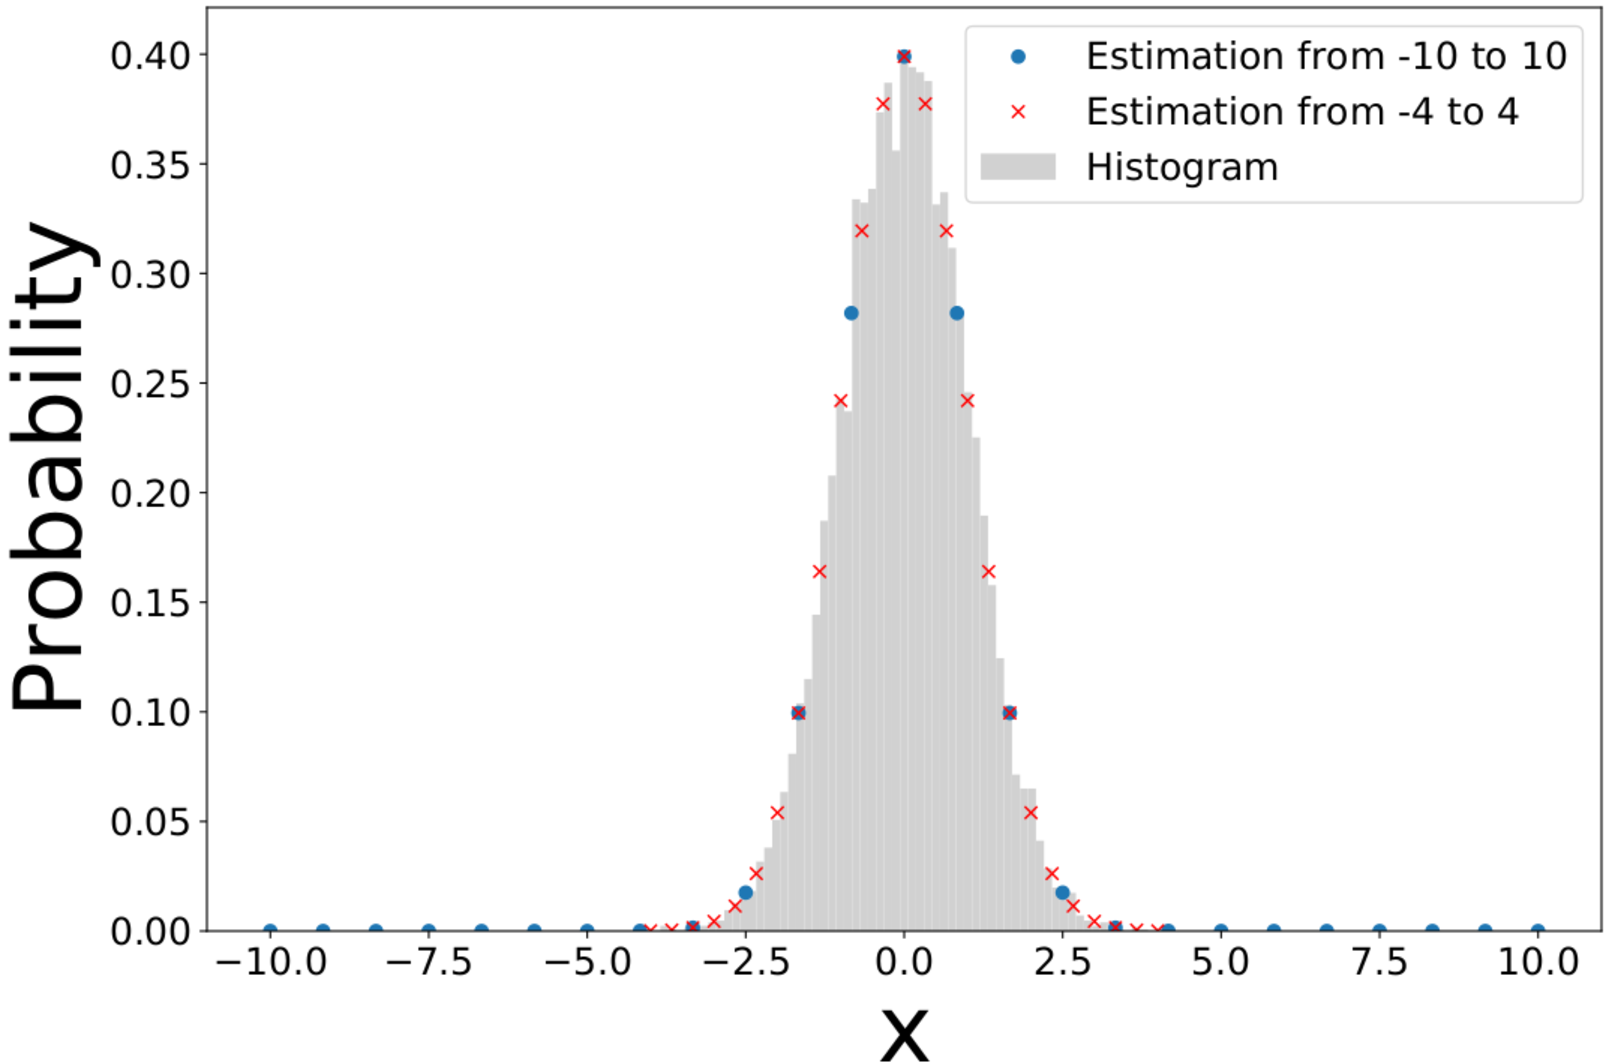
\includegraphics[width=0.6\linewidth]{figuras/linspace2}
	\caption{Caso representativo de estimação de PDF utilizando 25 pontos para dois intervalos diferentes (-4,4) e (-10,10)}
	\label{fig:figura1}
\end{figure}


\section{Métodos de Discretização} \label{cap:metodos}
Para se estudar os efeitos da discretização no processo de estimação de \ac{PDF}, a performance de cinco diferentes métodos serão confrontados, como listados abaixo: 
\begin{itemize}
	\item \textit{Linspace};
	\item \textit{CDFm};
	\item \textit{PDFm};
	\item \textit{iPDF1};
	\item \textit{iPDF2}.
\end{itemize}

Estes cinco métodos serão demostrados a priori  utilizando-se uma distribuição Gaussiana com média $\mu = 0$ e desvio padrão $\sigma = 1$, cuja \ac{PDF} pode ser descrita pela Equação~\eqref{equ:Normal} e ilustrada na Figura~\ref{fig:Gaussiana} com o numero de pontos $N = 25$ para uma melhor visualização.

\begin{equation}
{\displaystyle f_{X}(x;\mu,\sigma) = \frac{1}{\sigma\sqrt{2\pi}}\cdot e^{-\frac{(x-\mu)^2}{2\sigma^2}}}
\label{equ:Normal}
\end{equation}


\begin{figure}[H]
	\centering
	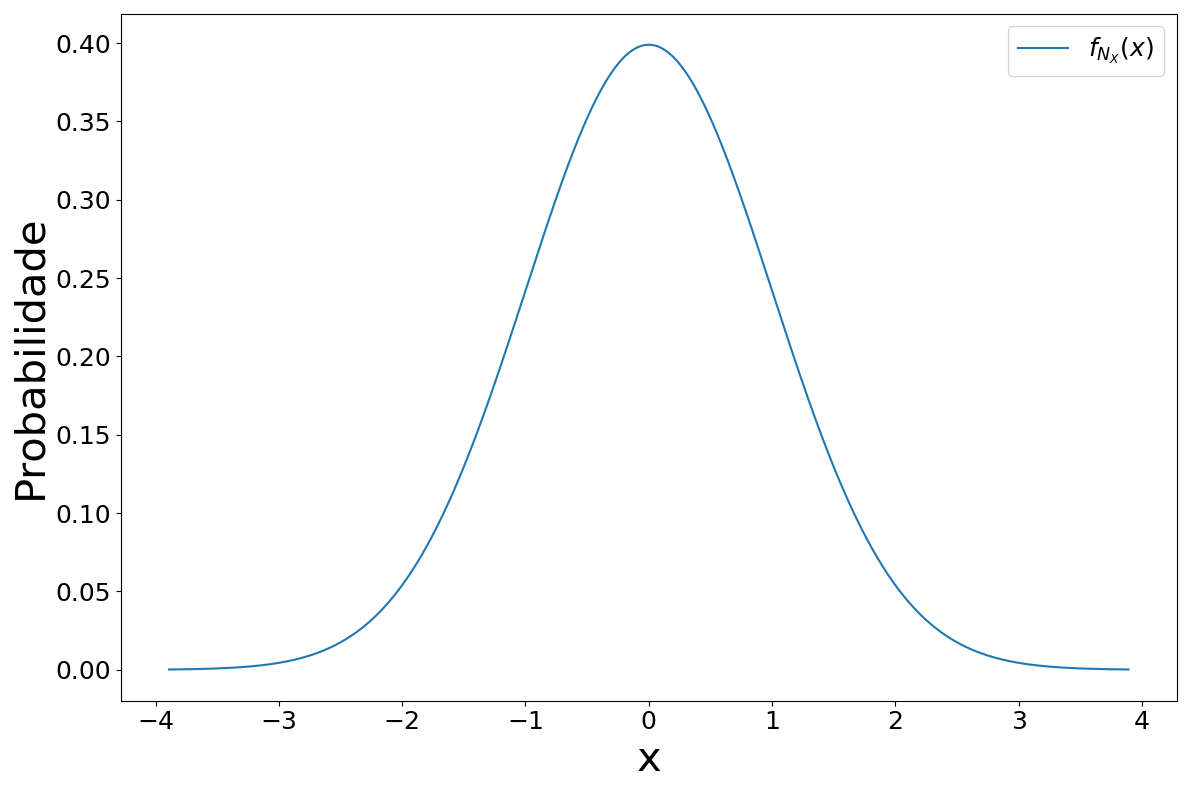
\includegraphics[width=0.6\linewidth]{./figuras/Normal}
	\caption{Ilustração da curva Gaussiana com média $\mu = 0$ e desvio padrão $\sigma = 1$.}
	\label{fig:Gaussiana}
\end{figure}

\subsection{\textit{Linspace}}
O método \textit{Linspace} é caracterizado por amostrar de maneira uniforme a variável aleatória, representada pelo eixo das abscissas de uma \ac{PDF} qualquer. Após, o eixo $ x $ terá \textit{N} pontos igualmente espaçados entre dois valores predefinidos que definem os parâmetros de início e término da distribuição. Este método é o mais utilizado na literatura devido a sua simplicidade. A Figura~\ref{fig:linspace_curve} ilustra o método \textit{Linspace} para a distribuição Normal, limitando o eixo horizontal à uma área de probabilidade de $99,99\%$.


\begin{figure}[H]
	\centering
	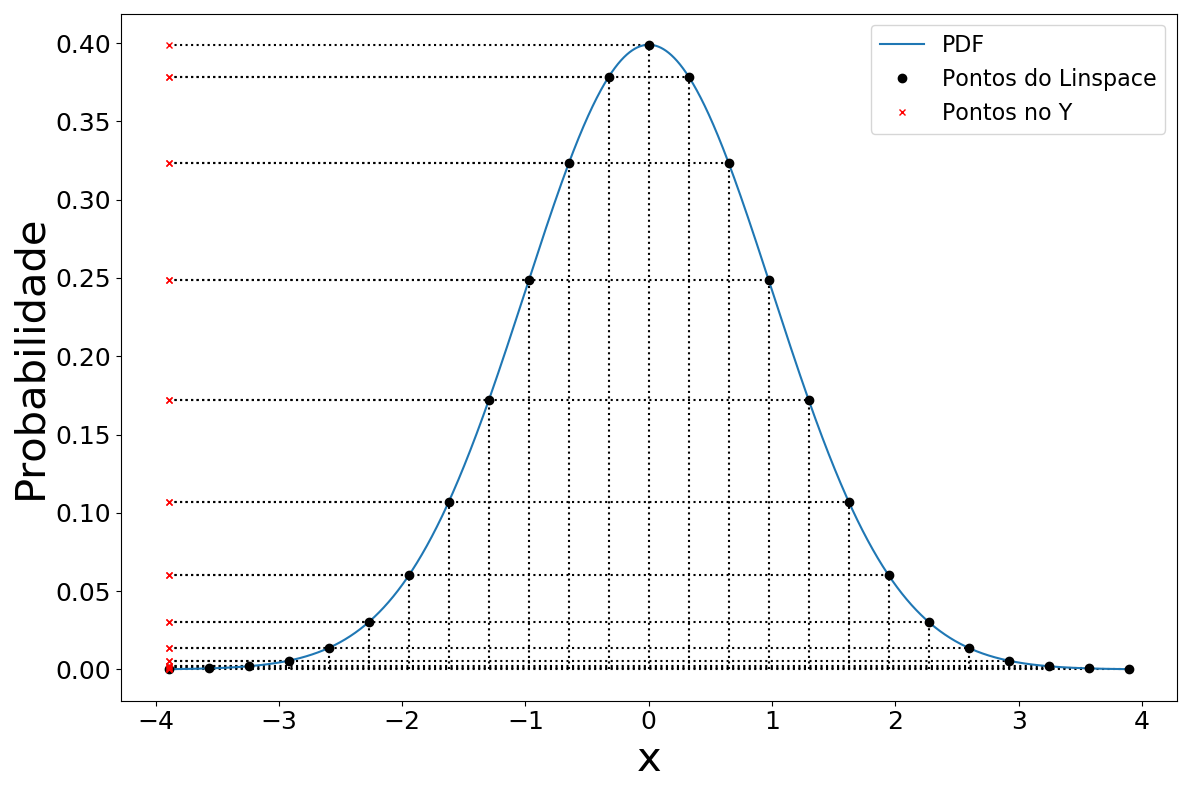
\includegraphics[width=0.7\linewidth]{./figuras/normal_1}
	\caption{Ilustração do método \textit{Linspace} aplicado à uma distribuição normal.}
	\label{fig:linspace_curve}
\end{figure}


\subsection{\textit{CDFm}}
O método denominado nesse trabalho de \ac{CDFm} representa a discretização baseada na \ac{CDF} descrita pela Equação~\eqref{equ:CDF} para uma variável contínua e \eqref{equ:CDF_disc} para o caso de uma variável discreta possuindo valores em $ b $. Para este método, no caso de se ter a função geradora, primeiramente calcula-se a \ac{CDF} da distribuição e então faz-se uma distribuição linear de pontos no eixo $ y $ e encontra-se os seus respectivos valores para o eixo $ x $ fazendo sua função inversa, conforme mostra a Equação~\eqref{equ:cdf_inv} e é ilustado pela Figura~\ref{fig:CDFm_curve}.


%a discretização baseada no espaçamento uniforme é aplicada ao eixo vertical e então os relativos valores horizontais são encontrados refletindo todos os valores, como mostra a Figura~\ref{fig:CDFm_curve} para a distribuição Normal. Note que, quanto maior a probabilidade da \ac{PDF}, maior o número de pontos na sua região.

\begin{equation}
\displaystyle F_X(x) = \int_{-\infty}^{x} f_X(t)dt
\label{equ:CDF}
\end{equation}

\begin{equation}
 {P} (X=b)=F_{X}(b)-\lim _{x\to b^{-}}F_{X}(x)
 \label{equ:CDF_disc}
\end{equation}

\begin{equation}
CDFm(y) = F^{-1}_X(x)
\label{equ:cdf_inv}
\end{equation}

\begin{figure}[H]
	\centering
	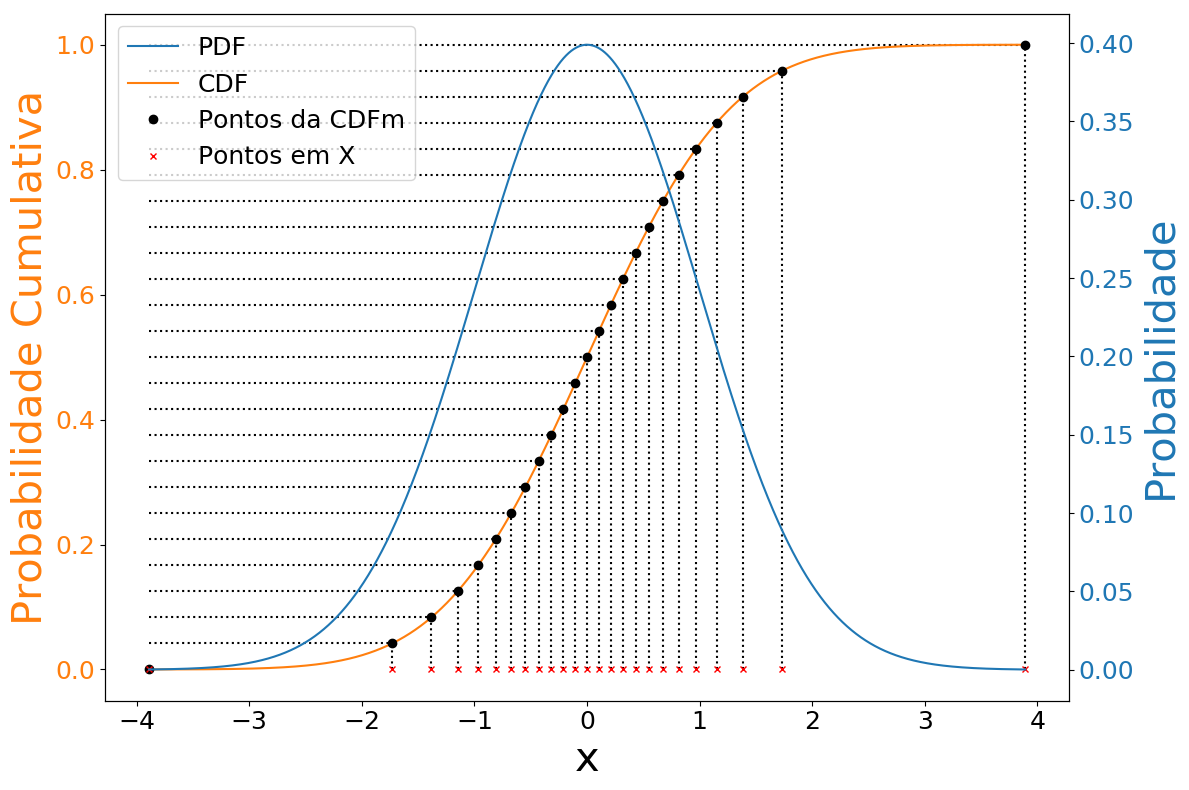
\includegraphics[width=0.6\linewidth]{./figuras/CDFm_normal_1}
	\caption{Ilustração da discretização da distribuição Gaussiana baseada em sua CDF.}
	\label{fig:CDFm_curve}
\end{figure}

É possível notar que, quanto maior a probabilidade da \ac{CDF}, maior o número de pontos em sua região.

\subsection{\textit{PDFm}}
Este método, denominado de \ac{PDFm} também usa a técnica de reflexão aplicada ao método da \textit{CDFm}, mas a função de referência é a própria \ac{PDF}, ao invés da sua \ac{CDF}, com isso, os pontos de intercessão da curva com os valores em $ y $ são calculados. A Figura~\ref{fig:PDFm_curve} mostra como este método funciona. 

\begin{figure}[H]
	\centering
	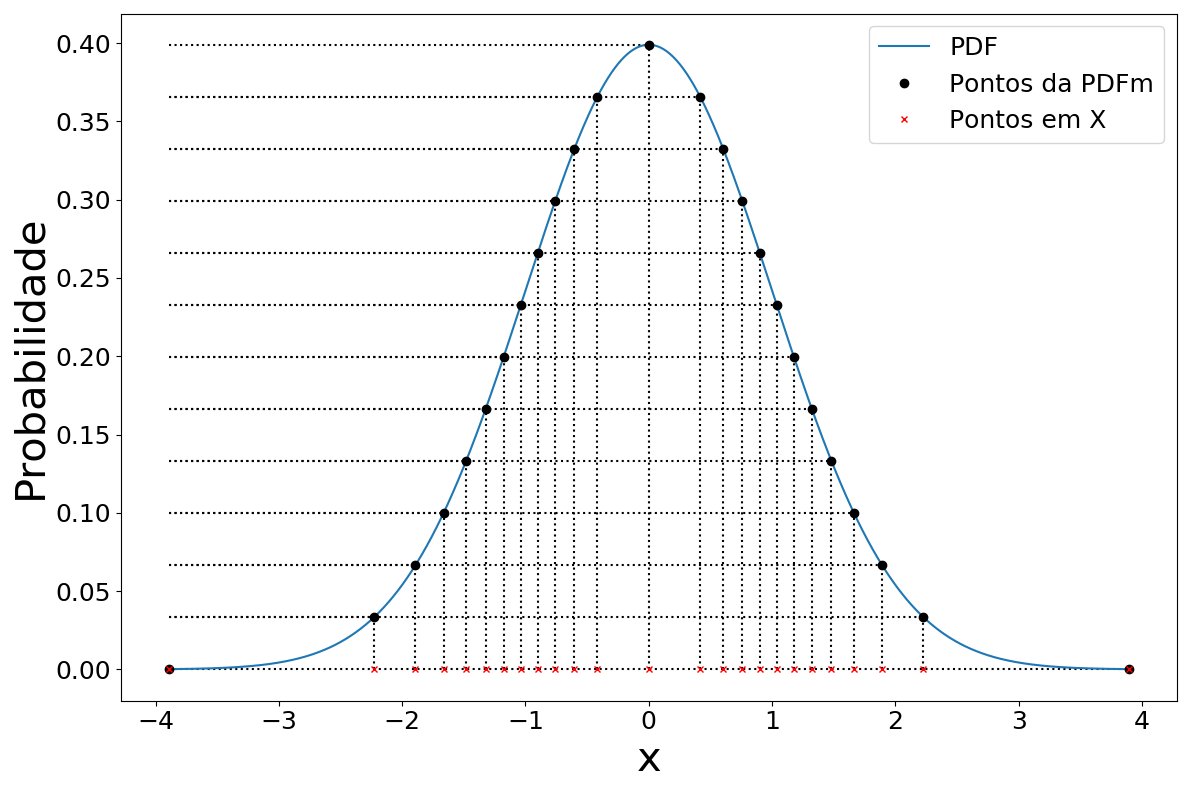
\includegraphics[width=0.67\linewidth]{./figuras/PDFm_normal_1}
	\caption{Ilustração da discretização da distribuição Gaussiana baseada em sua PDF.}
	\label{fig:PDFm_curve}
\end{figure}

Ela possui o efeito de incrementar o número de pontos estimados onde a inclinação da curva é mais acentuada.

\subsection{\textit{iPDF1}}

O método da \ac{iPDF1} reflete os valores verticais para o eixo horizontal usando a \ac{CDF} da primeira derivada da \ac{PDF} como uma transformação de base, como é ilustrado nas Figuras~\ref{fig:dPDF1} e \ref{fig:dPDF2}

\begin{figure}[!ht]
	\centering
	\begin{subfigure}[b]{0.44\textwidth}
		\centering 
		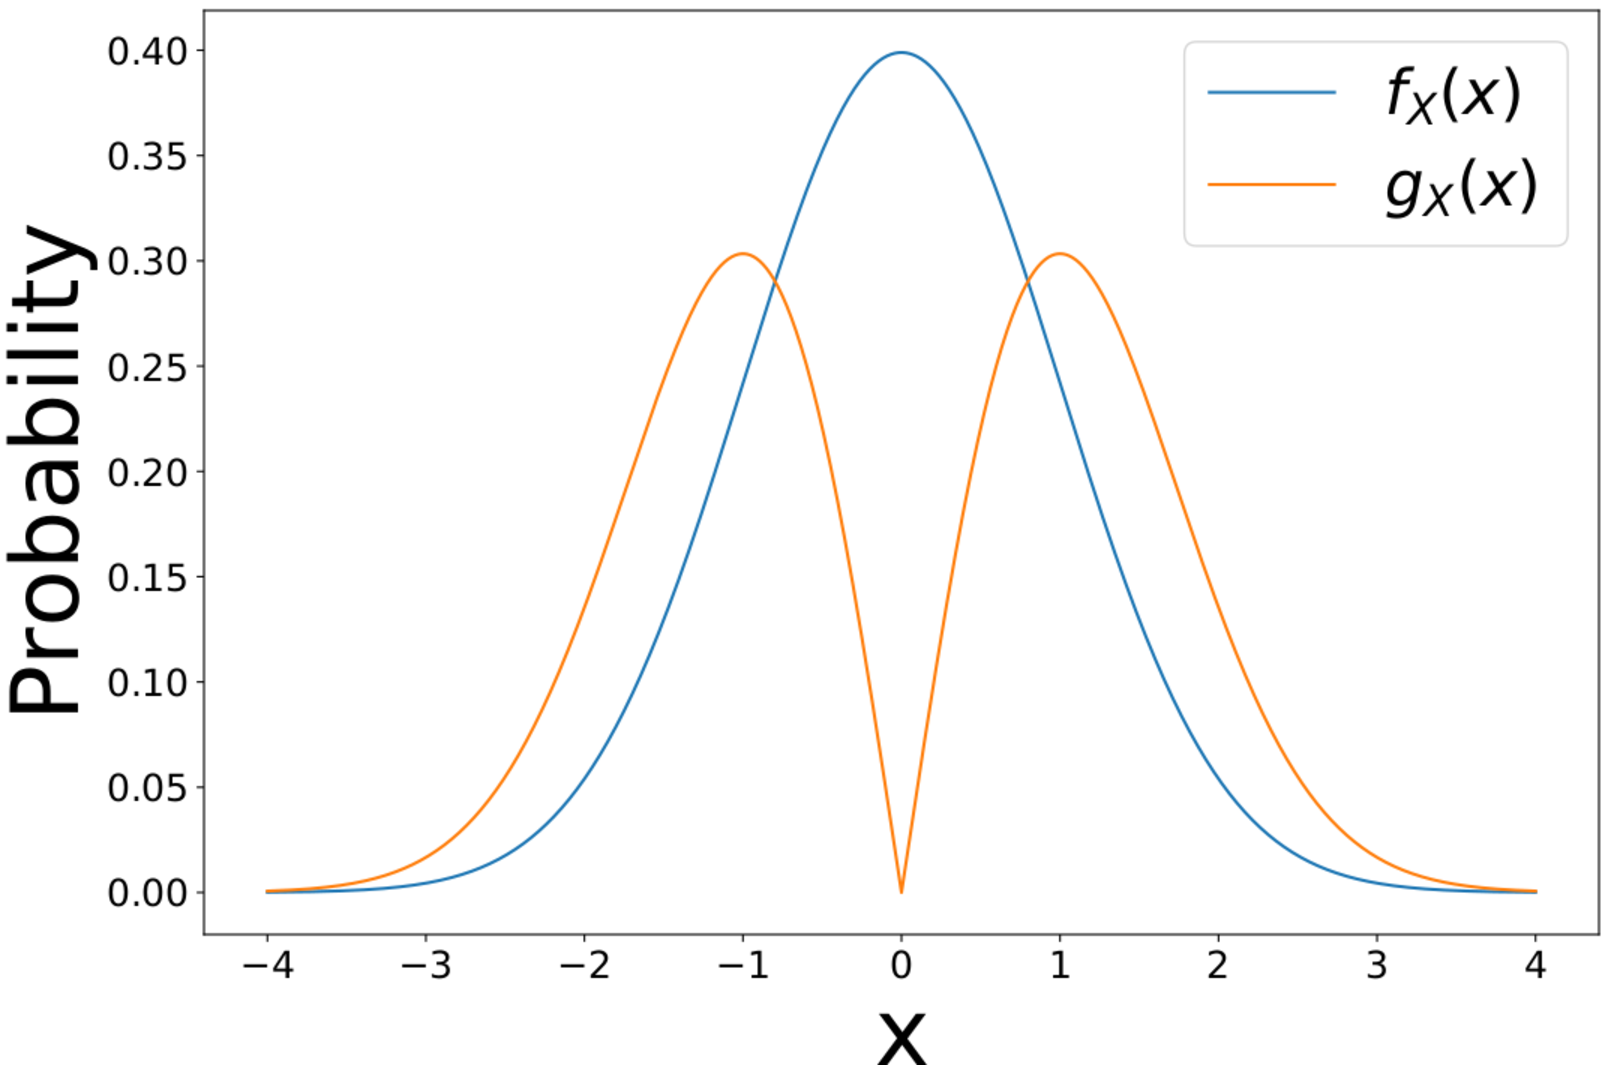
\includegraphics[width=\textwidth]{./figuras/dpdf1}
		\caption{}
		\label{fig:dPDF1}
	\end{subfigure}
	\hfill
	\begin{subfigure}[b]{0.47\textwidth}
		\centering 
		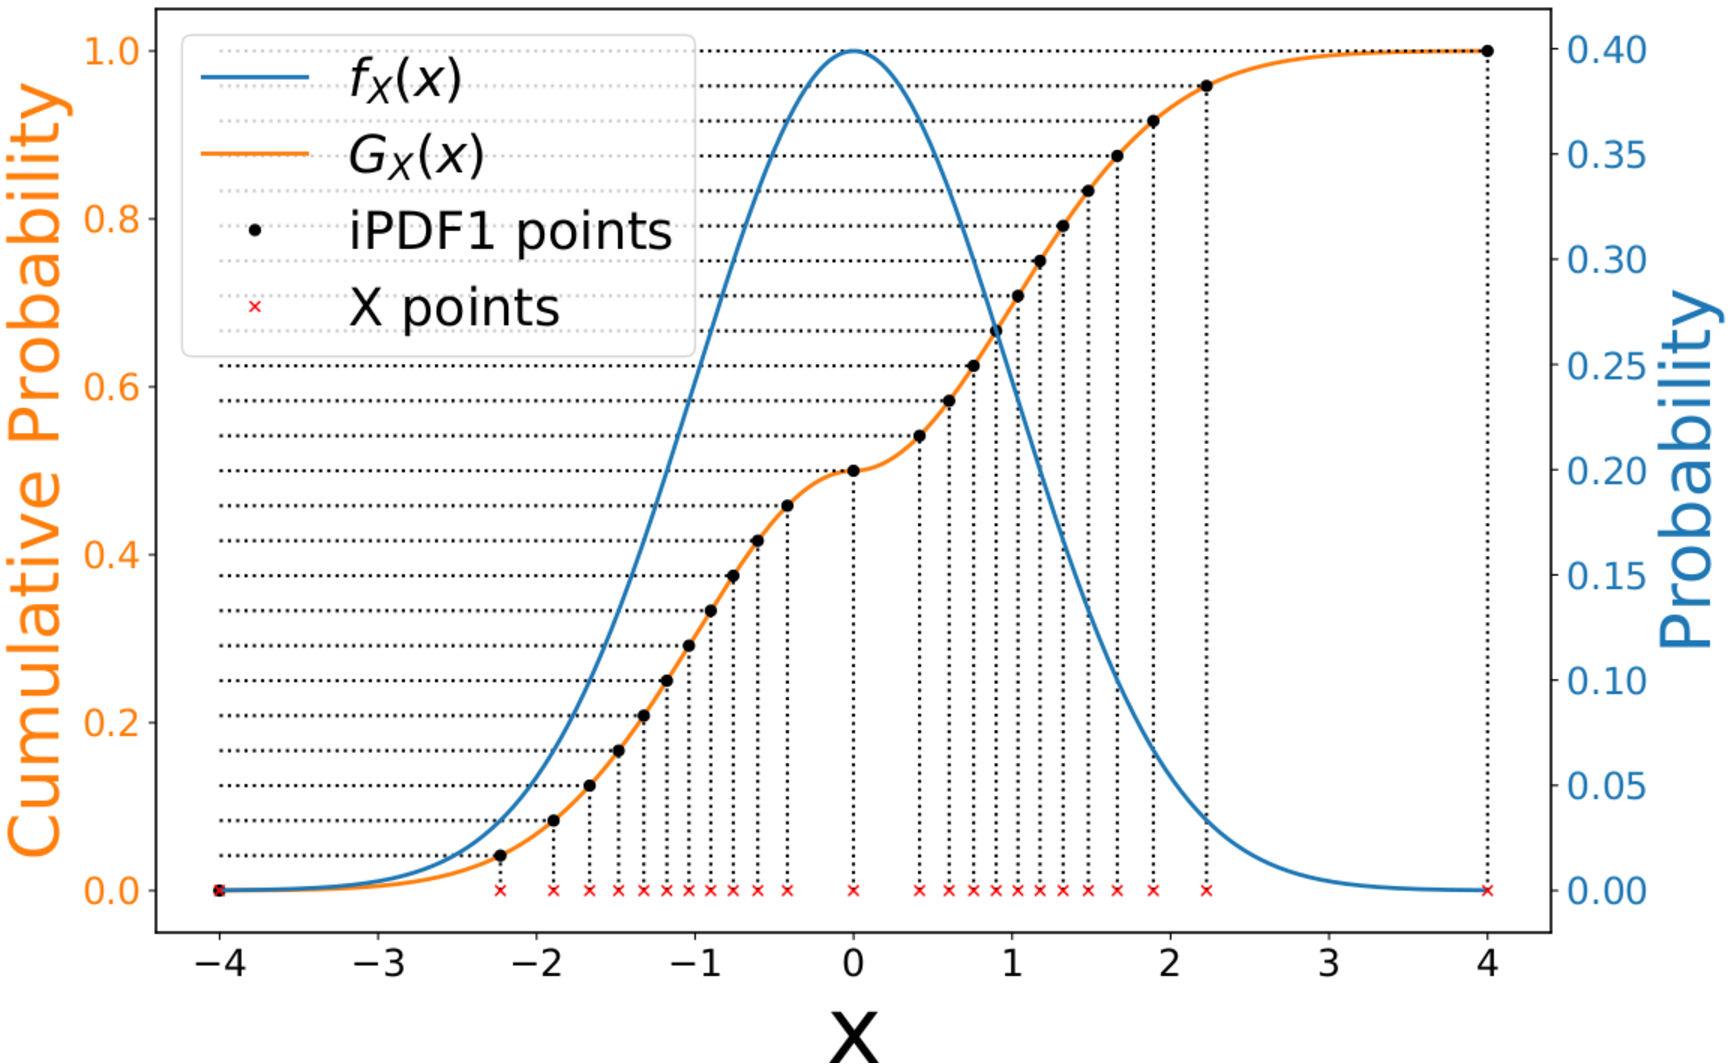
\includegraphics[width=\textwidth]{./figuras/dpdf2}
		\caption{}
		\label{fig:dPDF2}
	\end{subfigure}
	\caption{PDF Gaussiana e sua primeira derivada à esquerda. Ilustração da discretização da distribuição Gaussiana baseada na CDF da sua primeira derivada à direita.}
	\label{fig:dPDF}
\end{figure}

As equações \eqref{equ:dpdf1} e \eqref{equ:dcdf} descrevem este método matematicamente.

\begin{equation}
\begin{array}{l}
\vspace{0.3cm}\displaystyle \zeta(x) = \frac{|\mu-x|}{\sigma^3\sqrt{2\pi}}\cdot e^{\left(\frac{-(\mu-x)^2}{2\sigma^2}\right) } \\
\vspace{0.3cm} \displaystyle \int_{-\infty}^{\infty} \zeta(x)\cdot dx = c_1 \\
\displaystyle g_X(x) = \frac{\zeta(x)}{c_1}
\label{equ:dpdf1}
\end{array}
\end{equation}
onde $\zeta$ é a equação da distribuição da derivada da distribuição normal, $\mu$ é a média, $\sigma$ o desvio padrão, $x$ a variável aleatória, $c_1$ é a área abaixo da curva $\zeta$, e $g_X$ é a versão normalizada.	
A \ac{CDF} de $g_X$ ($G_X(x)$) é usada para transferir os valores da abscissa ao eixo da ordenada como mostra a  Figura~\ref{fig:dPDF2}.

\begin{equation}
G_X(x) = \int_{-\infty}^x g_X(y)\cdot dy
\label{equ:dcdf}
\end{equation}

É possível notar que este método consegue fazer uma melhor estimação nas regiões em que a primeira derivada de sua \ac{PDF} são maiores.

\subsection{\textit{iPDF2}}
Este método é construído da mesma maneira da \textit{IPDF1} mas usando a segunda derivada ao invés da primeira, como é mostrado na Figura~\ref{fig:ddPDF1} e \ref{fig:ddPDF2}. Suas equações são mostradas em \eqref{equ:hx} e \eqref{equ:ddcdf}.

\begin{figure}[ht]
	\centering
	\begin{subfigure}[b]{0.44\textwidth}
		\centering 
		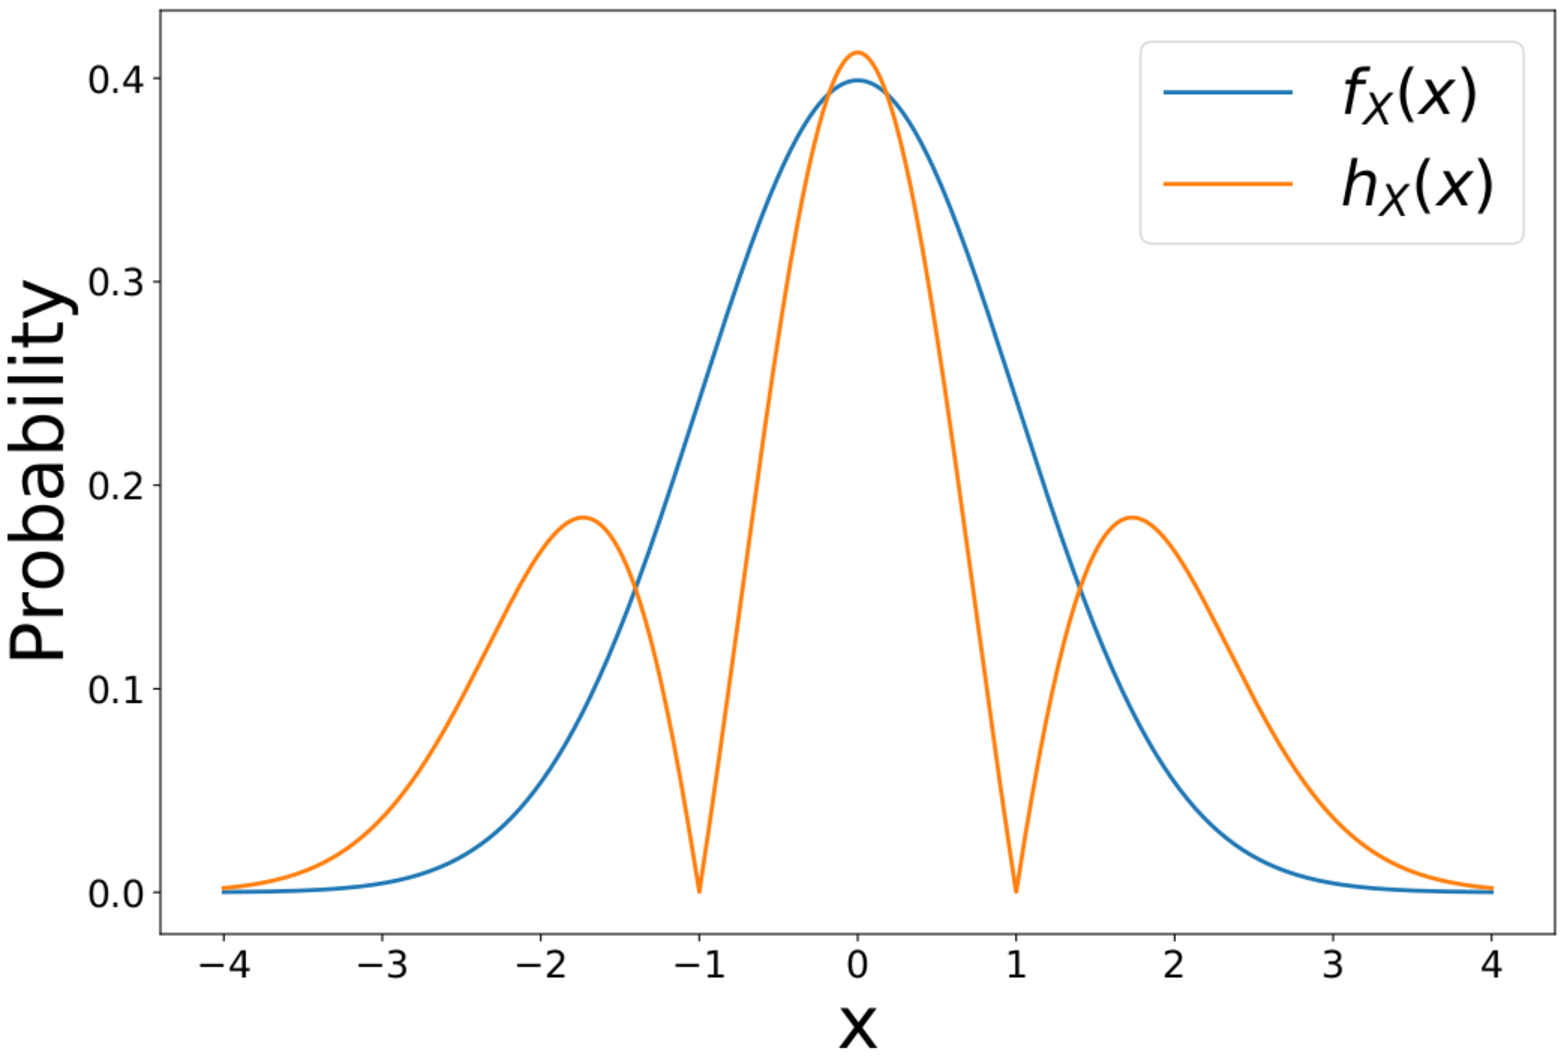
\includegraphics[width=\textwidth]{./figuras/ddpdf1.pdf}
		\caption{}
		\label{fig:ddPDF1}
	\end{subfigure}
	\hfill
	~ %add desired spacing between images, e. g. ~, \quad, \qquad, \hfill etc. 
	%(or a blank line to force the subfigure onto a new line)
	\begin{subfigure}[b]{0.47\textwidth}
		\centering 
		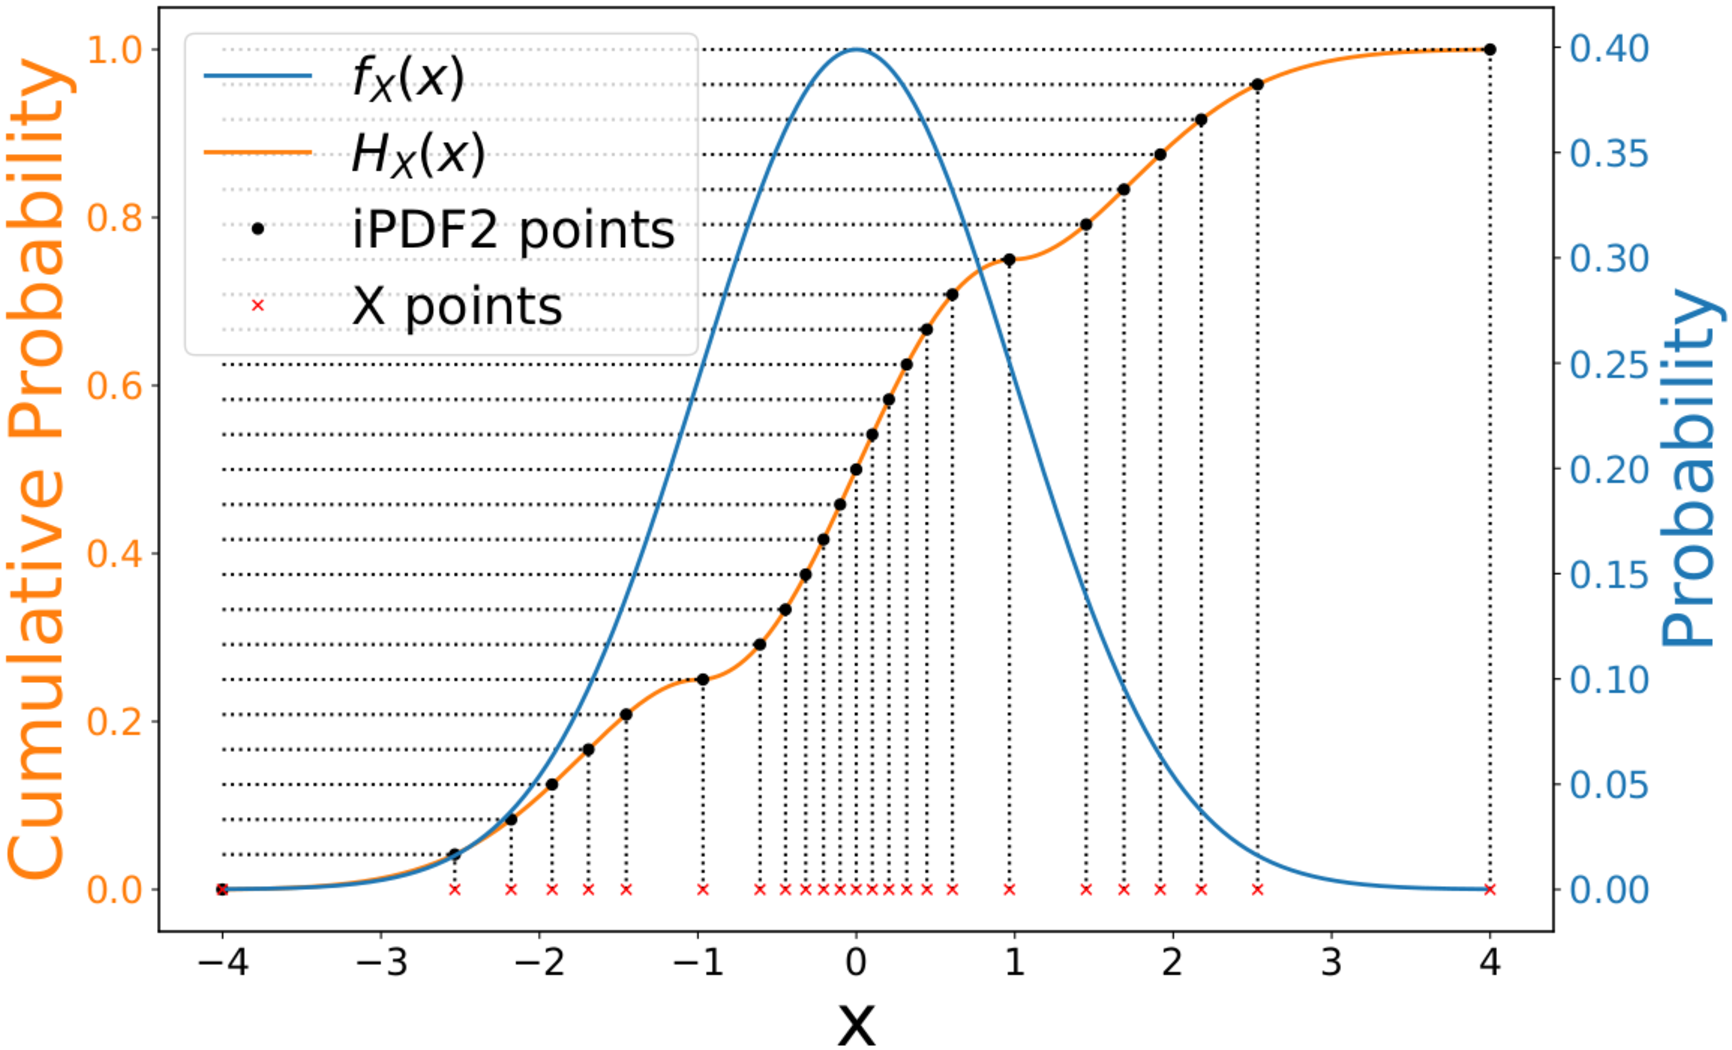
\includegraphics[width=\textwidth]{./figuras/ddpdf2.pdf}
		\caption{}
		\label{fig:ddPDF2}
	\end{subfigure}
	
	\caption{PDF Gaussiana e sua segunda derivada à esquerda. Ilustração da discretização da distribuição Gaussiana baseada na CDF da sua segunda derivada à direita.}
	\label{fig:ddPDF}
\end{figure}

\begin{equation}
\begin{array}{l}
\vspace{0.3cm}\displaystyle \eta(x) = \frac{|\sigma^2 - (\mu - x)^2|}{ \sigma^5\sqrt{2\pi}}\cdot e^{-\frac{(\mu - x)^2}{2 \sigma^2}} \\
\vspace{0.3cm} \displaystyle \int_{-\infty}^{\infty} \eta(x)\cdot dx = c_2 \\
\displaystyle h_X(x) = \frac{\eta(x)}{c_2}
\label{equ:hx}
\end{array}
\end{equation}
onde $\eta$ é a equação de distribuição de segunda derivada da distribuição Normal, $c_2$ é a área abaixo da curva desta distribuição, e $h_X$ é sua versão normalizada. 
Finalmente, $H_X(x)$ é a \ac{CDF} de $h_X$, dada por \eqref{equ:ddcdf}.

\begin{equation}
H_X(x) = \int_{-\infty}^x h_X(y)\cdot dy
\label{equ:ddcdf}
\end{equation}

Como é possível notar, há uma maior concentração de pontos onde a segunda derivada é maior.


Uma análise mais afunda sobre estes métodos será mostrada nos capítulos abaixo.

\chapter{DESENVOLVIMENTO} \label{cap:desenvolvimento}
Neste capítulo, será apresentado as propostas de métodos de discretização, sua descrição e equacionamento. Além disso, o contexto em que estes métodos serão avaliados também será mostrado.

Como o objetivo deste trabalho é validar apenas os efeitos da discretização no contexto da estimação de \ac{PDF}, o erro de estimação causado por este processo é medido entre a saída do processo de discretização em si e a função usada para gerar os dados. As funções aqui testadas serão baseadas em distribuições Gaussianas ou Lognormais com diferentes variâncias, bem como suas funções analíticas ou através de dados gerados.

\section{Métodos de discretização}
\label{cap:anal}
Para se estudar os efeitos da discretização no processo de estimação de \ac{PDF}, a performance de cinco diferentes métodos serão confrontados, como listados abaixo: 
\begin{itemize}
	\item \textit{Linspace};
	\item \textit{CDFm};
	\item \textit{PDFm};
	\item \textit{iPDF1};
	\item \textit{iPDF2}.
\end{itemize}

Estes cinco métodos serão mostrados utilizando \ac{PDF}s analíticas Gaussiana, com média $\mu = 0$ e desvio padrão $\sigma = 1$, descrita pela Equação~\eqref{equ:Normal} e ilustrada na Figura~\ref{fig:Gaussiana}, Lognormal, com $\mu = 0$ e desvio padrão $\sigma$ com valores $0.01, 0.25, 0.5, 1, 1.25$ e $1.5$, descrita pela Equação~\eqref{eq:Lognormal} e ilustrada na Figura~\ref{fig:Lognormal} e com três \textit{Datasets} diferentes, o primeiro sendo de uma distribuição normal com média nula e desvio padrão unitário representado na Figura~\ref{fig:randn}, o segundo será também uma distribuição normal com os mesmos parâmetros da primeira mas com a diferença que este irá possuir \textit{outliers}, ou seja, alguns pontos distantes da região de interesse ilustrado pela Figura~\ref{fig:randn_out} e, por fim, a ultima será uma distribuição Lognormal com média nula e desvio padrão de 0.5, ilustrado pela Figura~\ref{fig:randlog}. Todos os \textit{data sets} possuem mil eventos e foram gerados utilizando a biblioteca \textit{numpy} do \textit{software} \textit{Python} e com o número de \textit{binagem} definido pelo \ac{FD} que é um estimador robusto que leva em conta a variabilidade dos dados e o tamanho dos mesmos. Todos os métodos testados terão o número de estimação $N = 25$ para uma melhor visualização.

%Estes cinco métodos serão demostrados utilizando-se a \ac{PDF} Gaussiana com média $\mu = 0$ e desvio padrão $\sigma = 1$, descrita pela Equação~\eqref{equ:Normal} e ilustrada na Figura~\ref{fig:Gaussiana},  e a \ac{PDF} Lognormal com $\mu = 0$ e desvio padrão $\sigma$ com valores $0.01, 0.25, 0.5, 1, 1.25$ e $1.5$, descrita pela Equação~\eqref{eq:Lognormal} e ilustrada na Figura~\ref{fig:Lognormal}, além disso, estes métodos também s ambas com o numero de pontos $N = 25$.
  
\begin{equation}
{\displaystyle f_{N_X}(x;\mu,\sigma) = \frac{1}{\sigma\sqrt{2\pi}}\cdot e^{-\frac{(x-\mu)^2}{2\sigma^2}}}
\label{equ:Normal}
\end{equation}

\begin{equation}
	{\displaystyle f_{L_X}(x;\mu ,\sigma )={\frac {1}{x\sigma {\sqrt {2\pi }}}}\cdot e^ {-\frac {\left(\ln(x)-\mu \right)^{2}}{2\sigma ^{2}}}}
	\label{eq:Lognormal}
\end{equation}
onde $\mu$ é a média da distribuição, $\sigma$ o desvio padrão e $x$ a variável aleatória.

\begin{figure}[H]
	\centering
	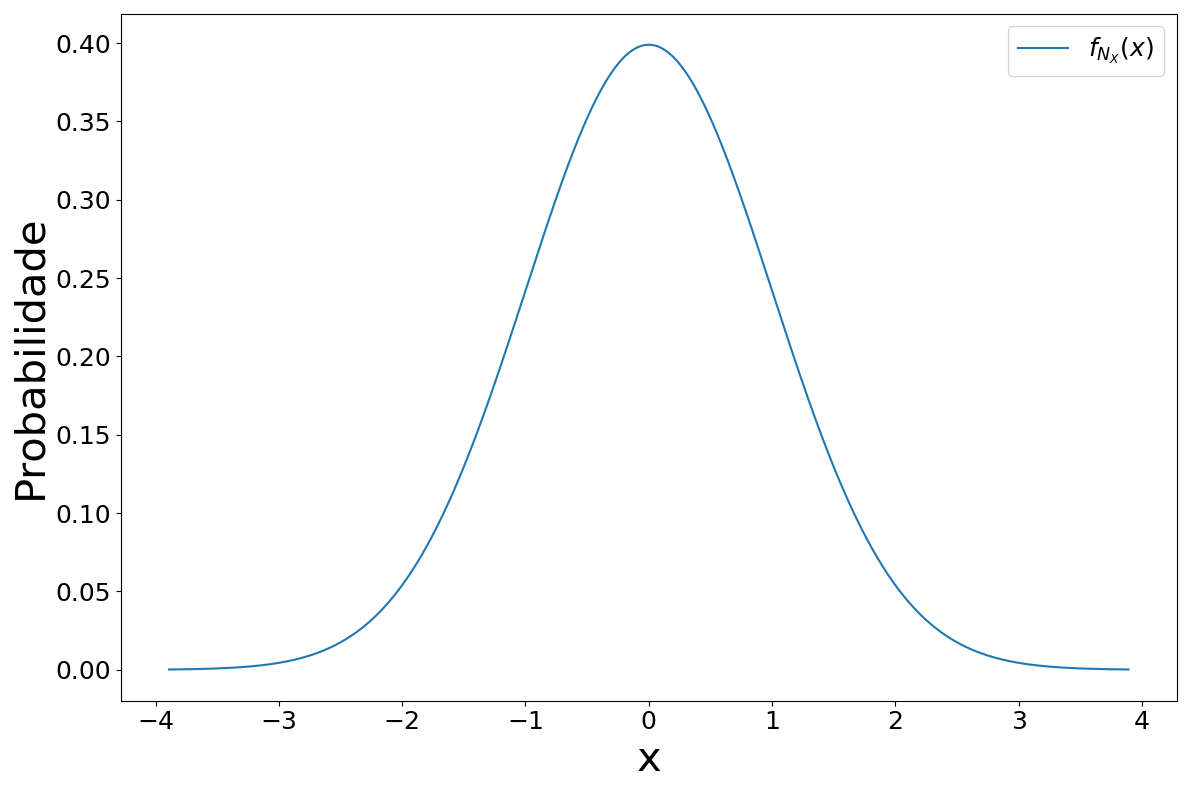
\includegraphics[width=0.8\linewidth]{./figuras/Normal}
	\caption{Ilustração da curva Gaussiana com média $\mu = 0$ e desvio padrão $\sigma = 1$.}
	\label{fig:Gaussiana}
\end{figure}

\begin{figure}[H]
	\centering
	\begin{subfigure}[b]{0.3\textwidth}
		\centering 
		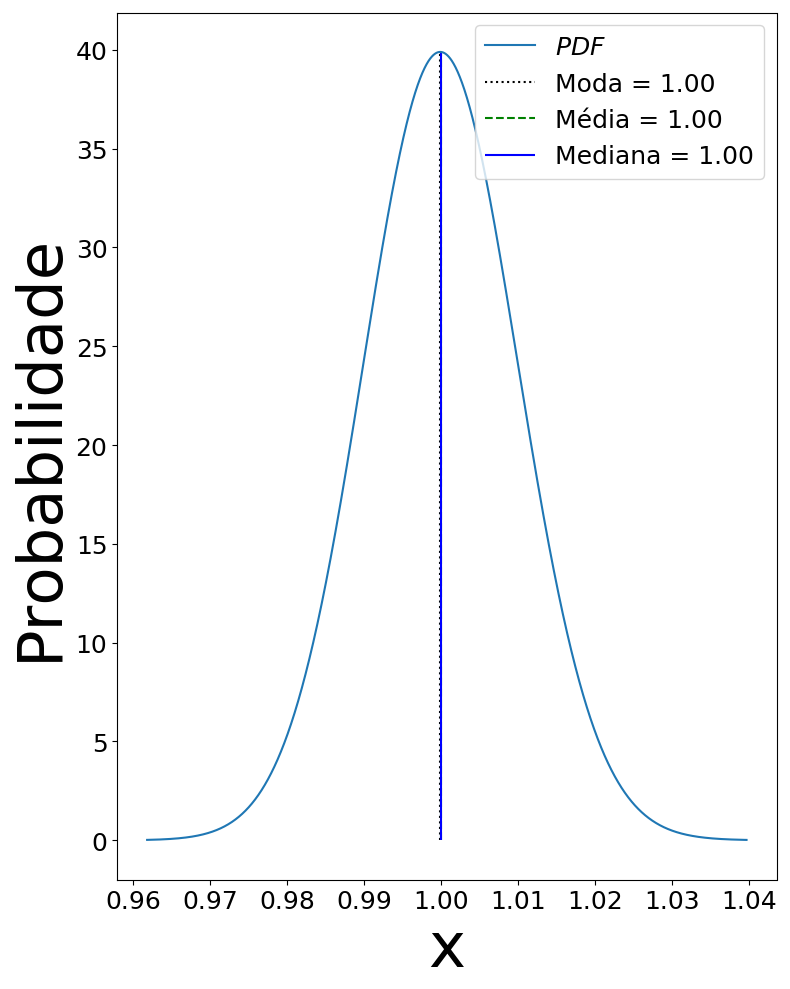
\includegraphics[width=\textwidth]{./figuras/log_sigma_001.png}
		\caption{}
		\label{fig:sig001}
	\end{subfigure}
	\hfill
	\begin{subfigure}[b]{0.3\textwidth}
		\centering 
		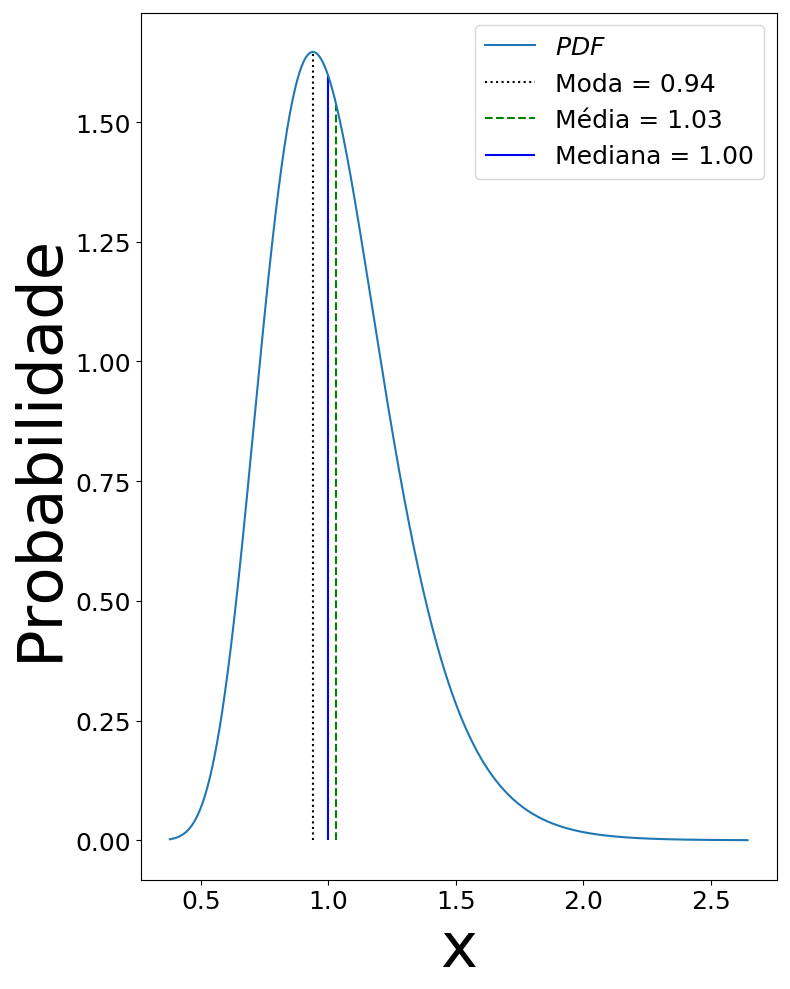
\includegraphics[width=\textwidth]{./figuras/log_sigma_025}
		\caption{}
		\label{fig:sig025}
	\end{subfigure}
	\hfill
	\begin{subfigure}[b]{0.3\textwidth}
		\centering 
		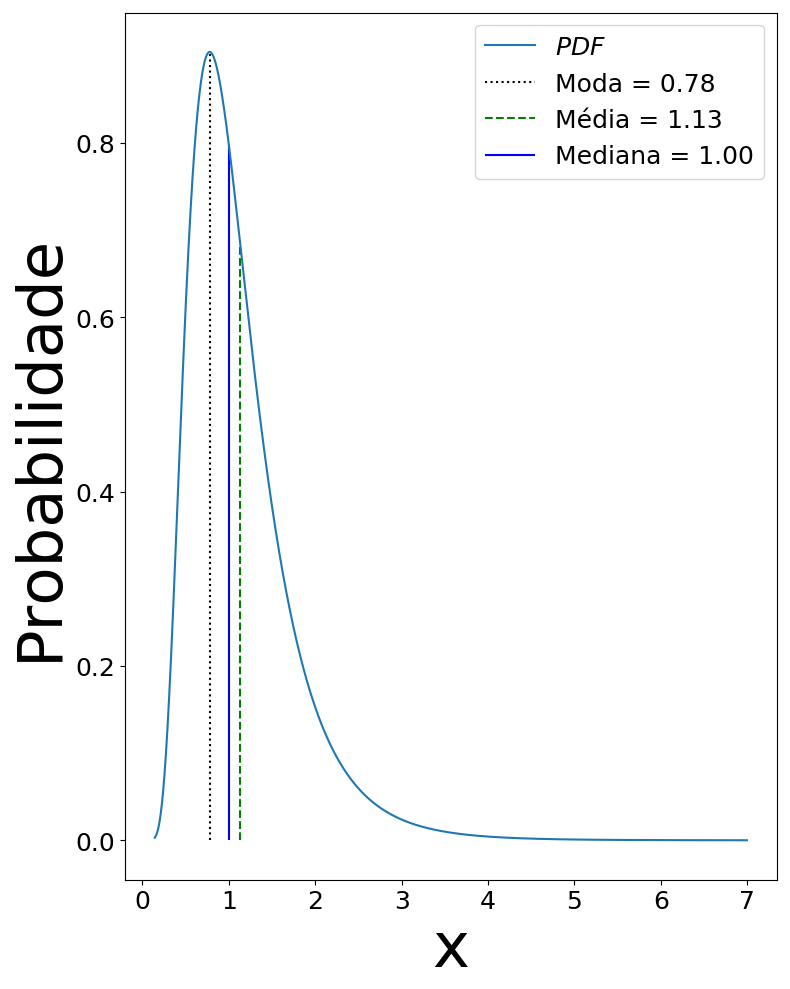
\includegraphics[width=\textwidth]{./figuras/log_sigma_05}
		\caption{}
		\label{fig:sig050}
	\end{subfigure}
	
	\begin{subfigure}[b]{0.3\textwidth}
		\centering 
		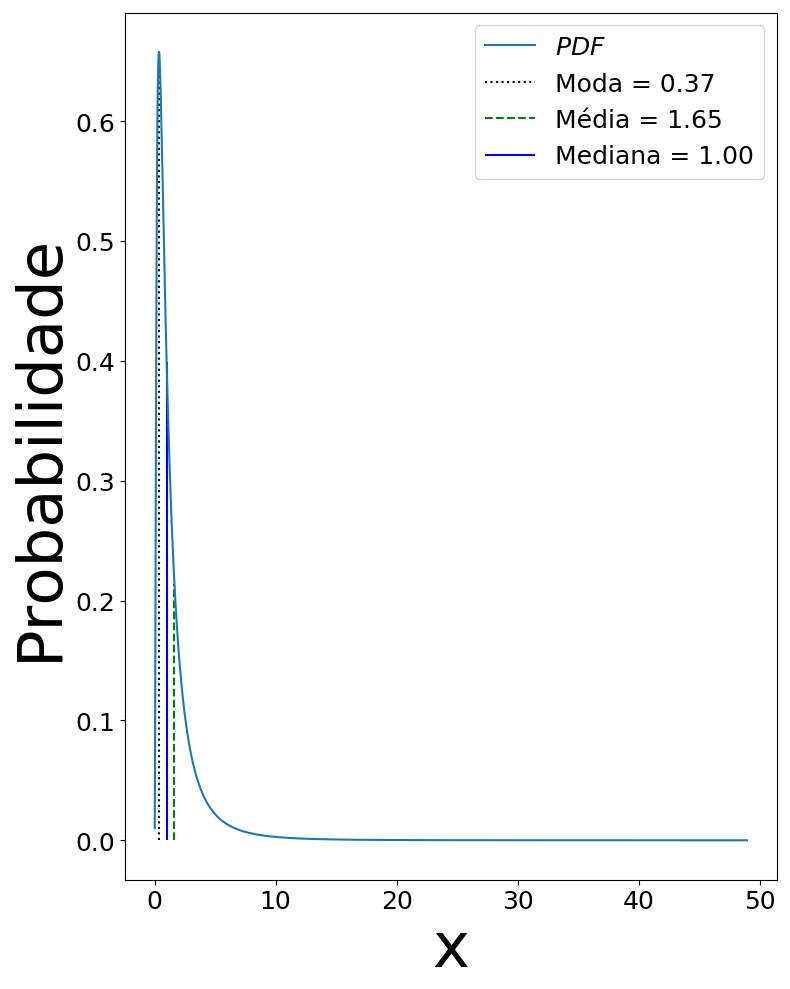
\includegraphics[width=\textwidth]{./figuras/log_sigma_1}
		\caption{}
		\label{fig:sig100}
	\end{subfigure}
	\hfill
	\begin{subfigure}[b]{0.3\textwidth}
		\centering 
		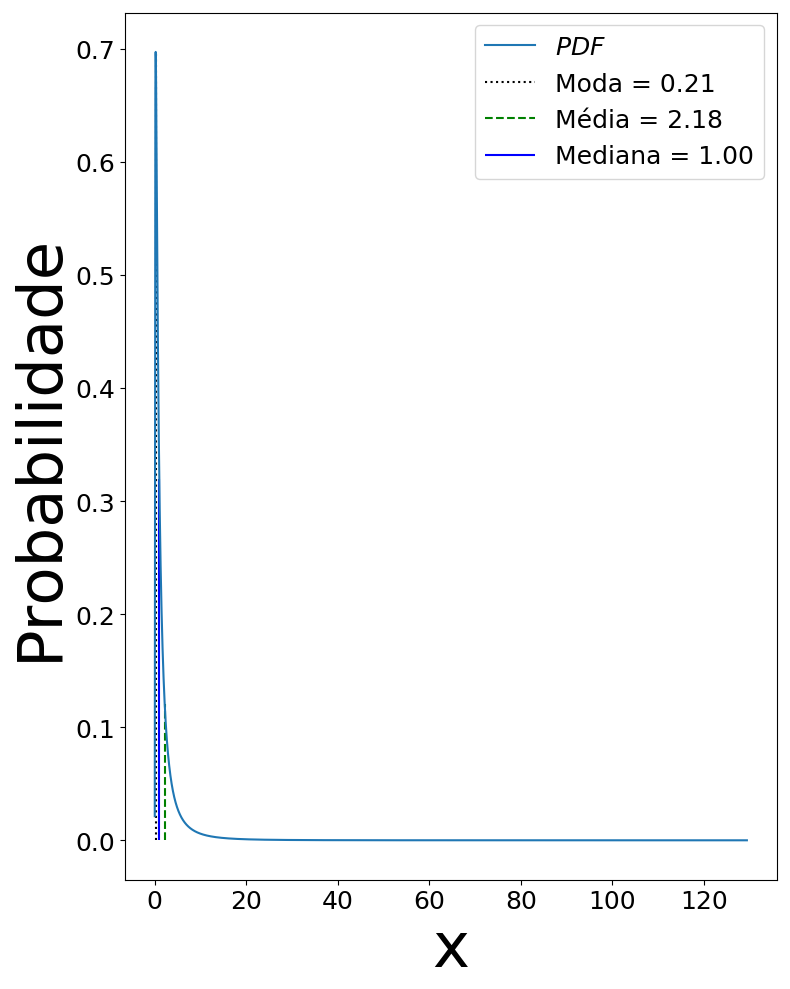
\includegraphics[width=\textwidth]{./figuras/log_sigma_125}
		\caption{}
		\label{fig:sig125}
	\end{subfigure}
	\hfill
	\begin{subfigure}[b]{0.3\textwidth}
		\centering 
		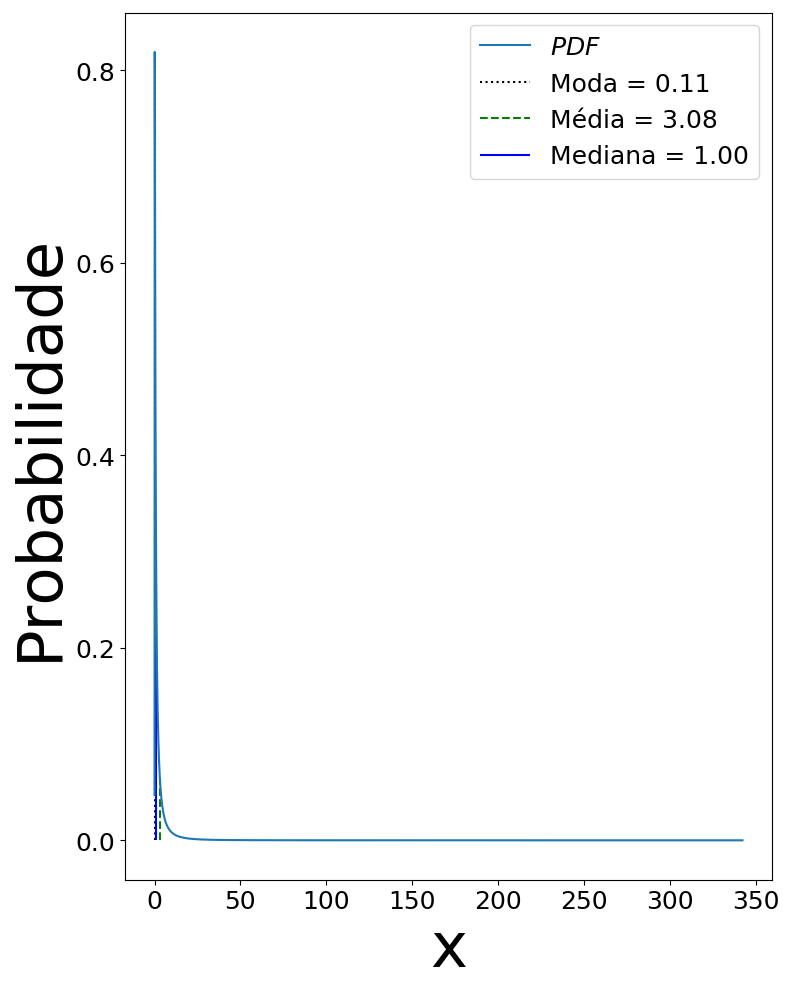
\includegraphics[width=\textwidth]{./figuras/log_sigma_15}
		\caption{}
		\label{fig:sig150}
	\end{subfigure}
	
	\caption{Ilustração das curvas Lognormais em que: (a) possui $\sigma = 0.01$; (b) possui $\sigma = 0.25$; (c) possui $\sigma = 0.5$; (d) possui $\sigma = 1$; (e) possui $\sigma = 1.25$; e (f) possui $\sigma = 1.5$}
	\label{fig:Lognormal}
\end{figure}



\begin{figure}[H]
	\centering
	\begin{subfigure}[b]{0.27\textwidth}
		\centering 
		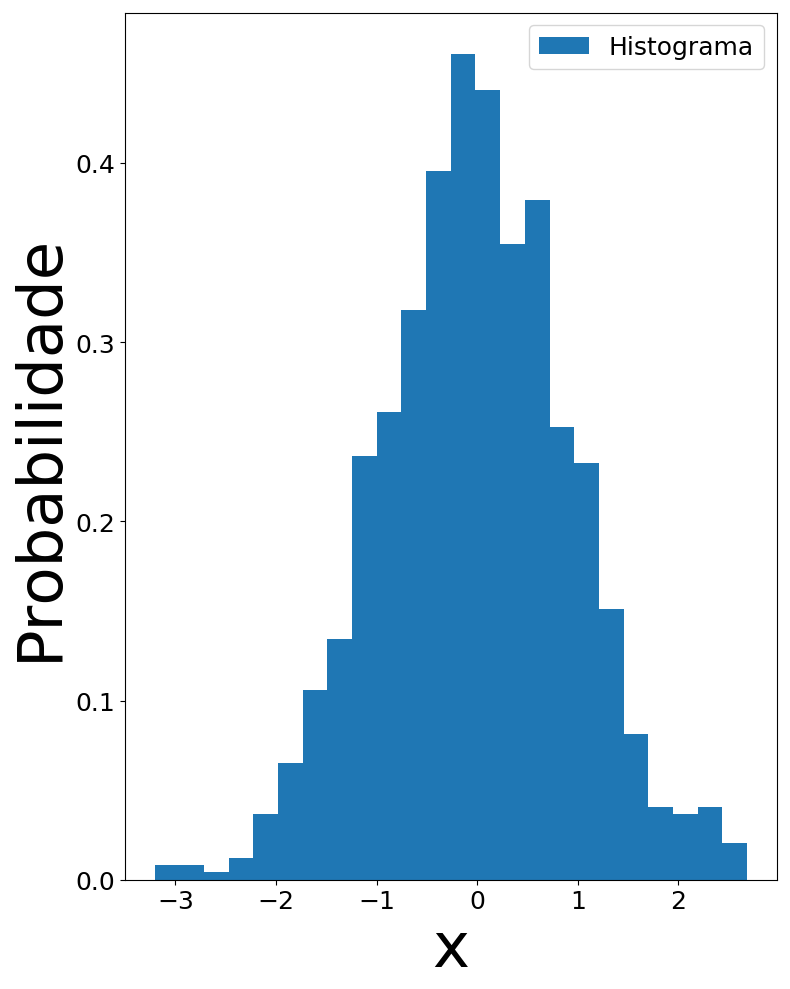
\includegraphics[width=\linewidth]{./figuras/datanormal_0}
		\caption{}
		\label{fig:randn}
	\end{subfigure}
	\hfill
	\begin{subfigure}[b]{0.27\textwidth}
		\centering 
		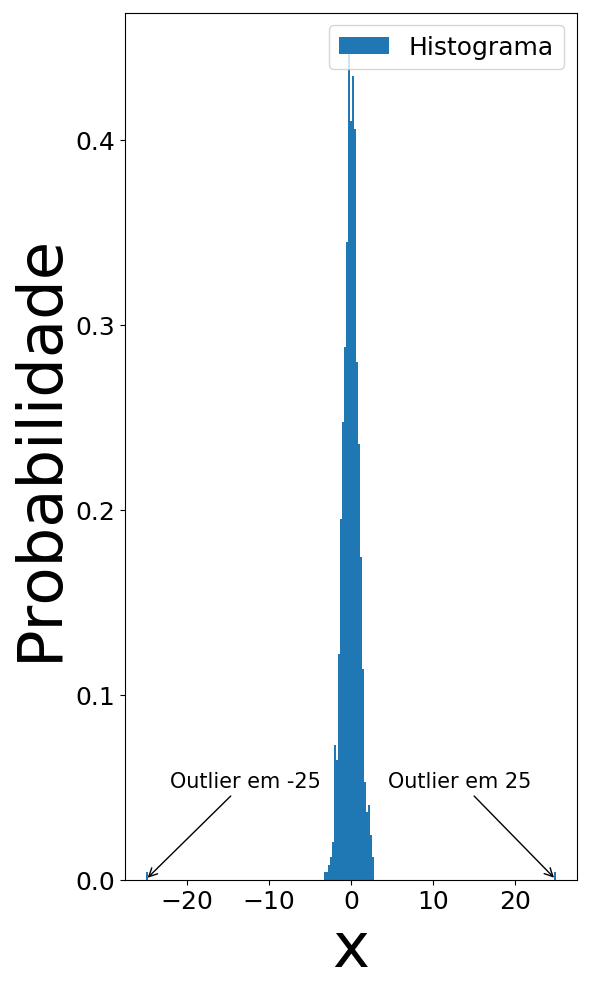
\includegraphics[width=\linewidth]{./figuras/datanormal_25}
		\caption{}
		\label{fig:randn_out}
	\end{subfigure}
	\hfill
	\begin{subfigure}[b]{0.27\textwidth}
		\centering 
		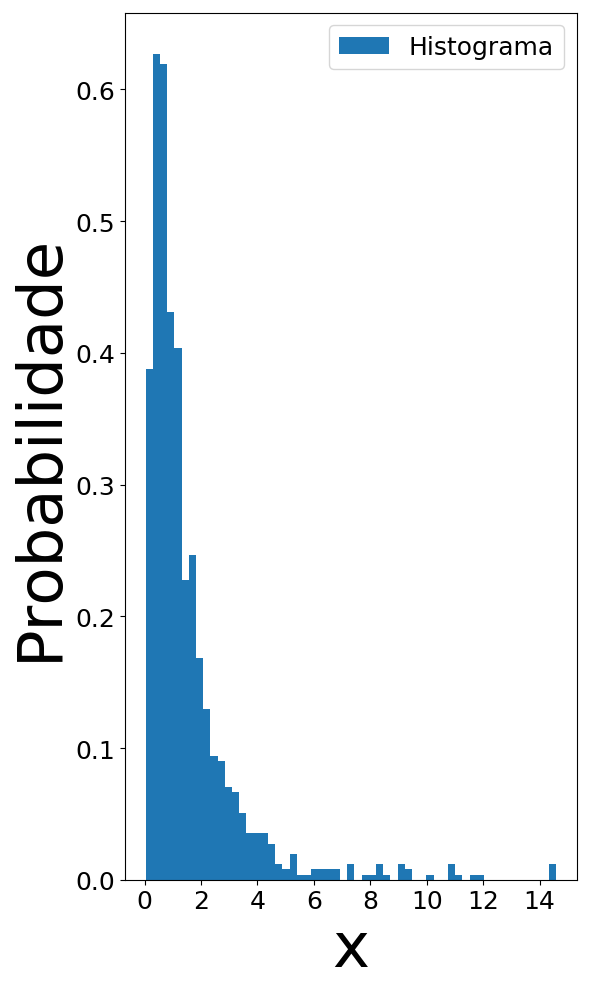
\includegraphics[width=\linewidth]{./figuras/datalognormal_0}
		\caption{}
		\label{fig:randlog}
	\end{subfigure}
	
	\caption{Histograma dos dados gerados sendo eles: (a) Gaussiana com $\mu = 0$ e $\sigma$ = 1; (b) Gaussiana com $\mu = 0$, $\sigma = 1$ e \textit{outlier} em $\pm 25$; (c) Lognormal com $\mu = 0$ e $\sigma = 0.5$.}
	\label{fig:data}
\end{figure}


\subsection{\textit{Linspace}}
O método \textit{Linspace} é caracterizado por amostrar de maneira uniforme a variável aleatória, representada pelo eixo das abscissas de uma \ac{PDF} dada. Após, o eixo horizontal terá \textit{N} pontos igualmente espaçados entre dois valores predefinidos que definem os parâmetros de início e término da distribuição. Este método é o mais utilizado na literatura devido a sua simplicidade. A Figura~\ref{fig:linspace_curve} ilustra o método \textit{Linspace} para a distribuição Normal e a Figura~\ref{fig:Lognormal_lin} ilustra o mesmo método para uma distribuição Lognormal com diferentes desvios padrões, limitando o eixo horizontal à uma área de probabilidade de $99.99\%$. A Figura~\ref{fig:datalin} mostra as distribuições geradas, conforme é mostrada na Figura~\ref{fig:data}, discretizadas utilizando este método.

\begin{figure}[H]
	\centering
	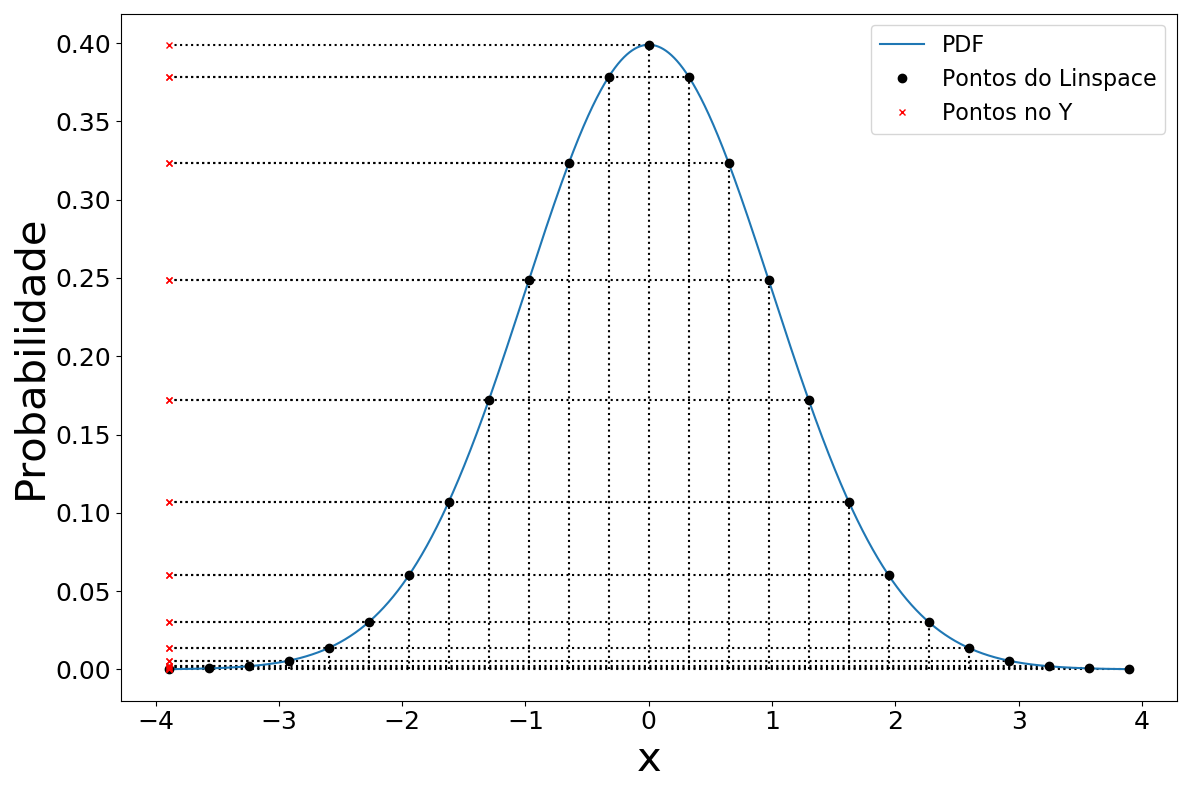
\includegraphics[width=0.7\linewidth]{./figuras/normal_1}
	\caption{Ilustração do método Linspace aplicado à uma distribuição normal.}
	\label{fig:linspace_curve}
\end{figure}

\begin{figure}[H]
	\centering
	\begin{subfigure}[b]{0.3\textwidth}
		\centering 
		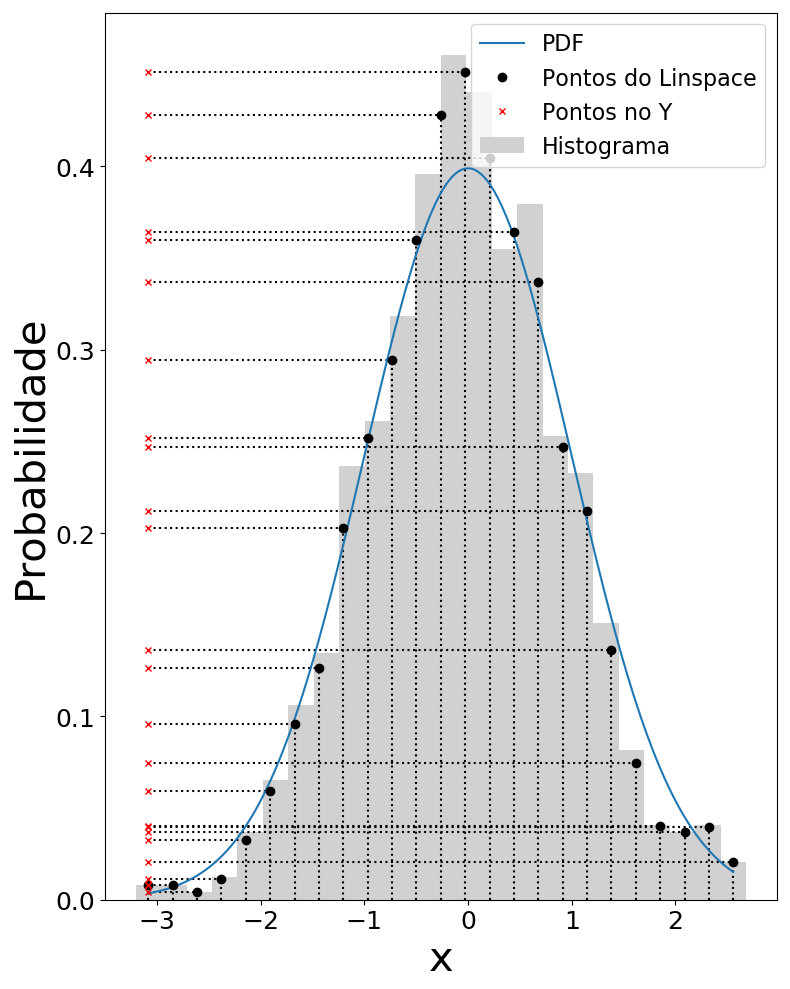
\includegraphics[width=\linewidth]{./figuras/normal_1_0}
		\caption{}
		\label{fig:randnlin}
	\end{subfigure}
	\hfill
	\begin{subfigure}[b]{0.3\textwidth}
		\centering 
		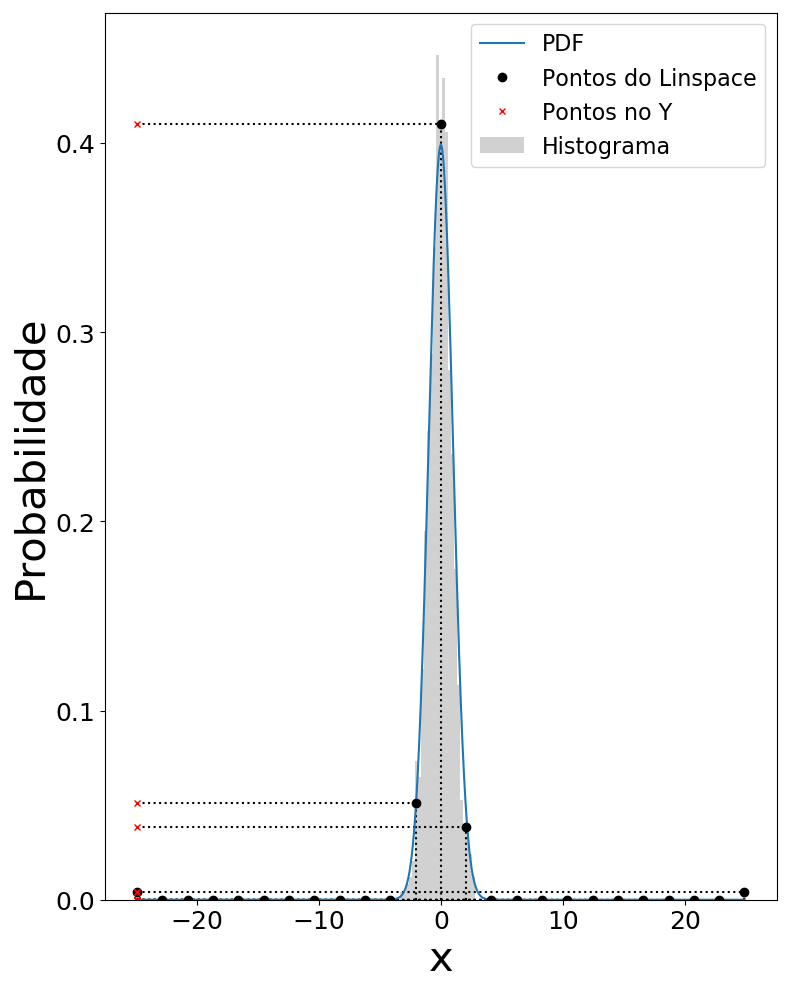
\includegraphics[width=\linewidth]{./figuras/normal_1_25}
		\caption{}
		\label{fig:randn_outlin}
	\end{subfigure}
	\hfill
	\begin{subfigure}[b]{0.3\textwidth}
		\centering 
		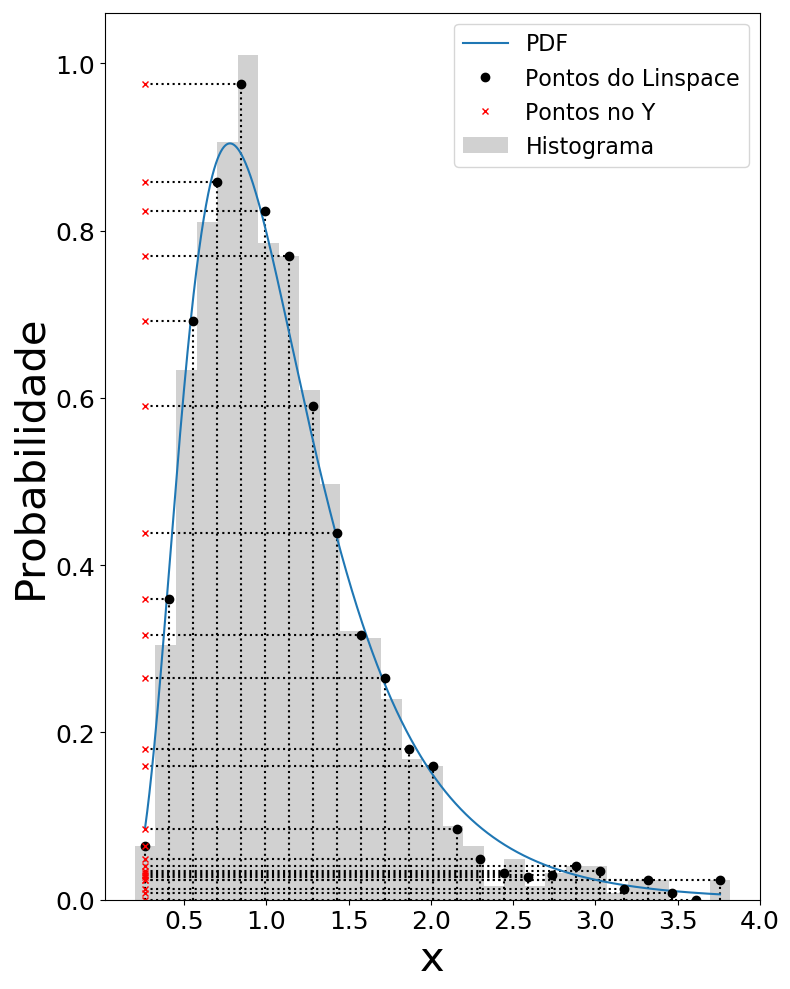
\includegraphics[width=\linewidth]{./figuras/lognormal_05_0}
		\caption{}
		\label{fig:randloglin}
	\end{subfigure}
	
	\caption{Histograma dos dados gerados utilizando a discretização pelo método \textit{Linspace} sendo eles: (a) Gaussiana com $\mu = 0$ e $\sigma$ = 1; (b) Gaussiana com $\mu = 0$, $\sigma = 1$ e \textit{outlier} em $\pm 25$; (c) Lognormal com $\mu = 0$ e $\sigma = 0.5$.}
	\label{fig:datalin}
\end{figure}


\begin{figure}[H]
	\centering
	\begin{subfigure}[b]{0.3\textwidth}
		\centering 
		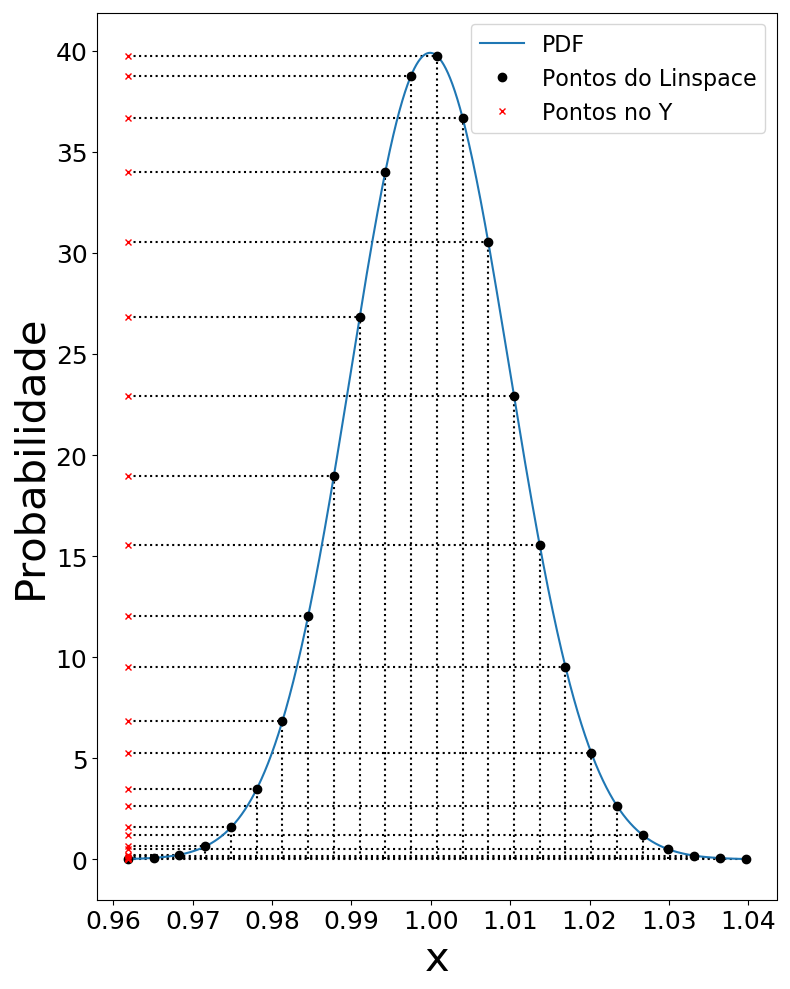
\includegraphics[width=\textwidth]{./figuras/lognormal_001.png}
		\caption{}
		\label{fig:lin001}
	\end{subfigure}
	\hfill
	\begin{subfigure}[b]{0.3\textwidth}
		\centering 
		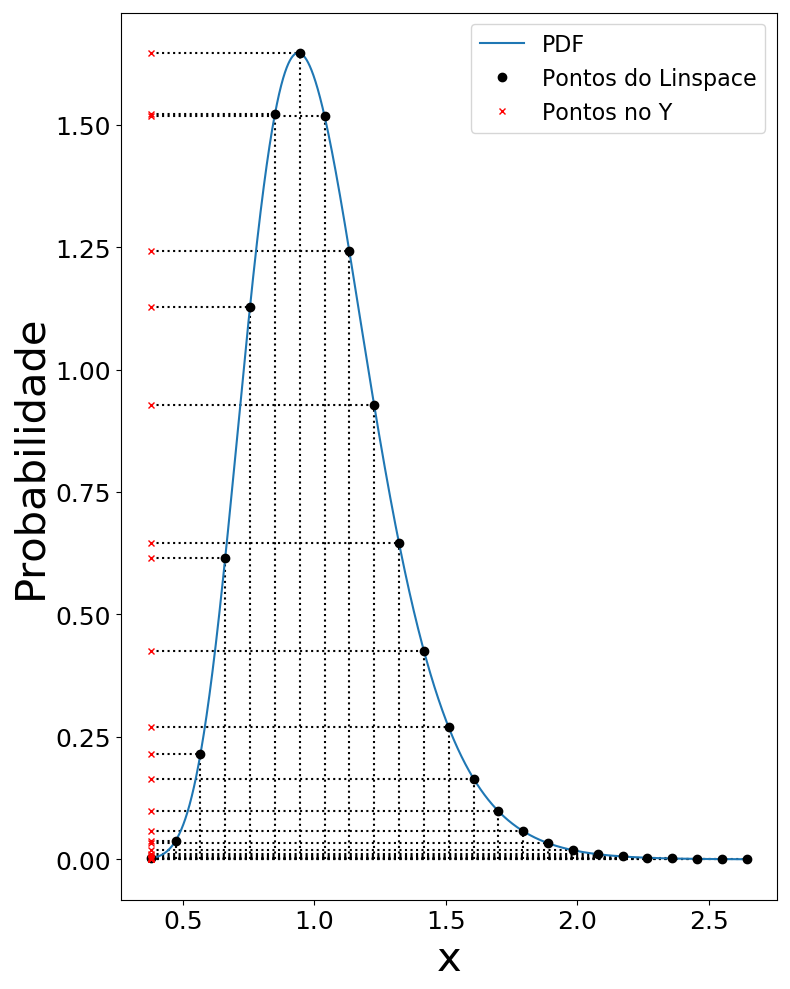
\includegraphics[width=\textwidth]{./figuras/lognormal_025}
		\caption{}
		\label{fig:lin025}
	\end{subfigure}
	\hfill
	\begin{subfigure}[b]{0.3\textwidth}
		\centering 
		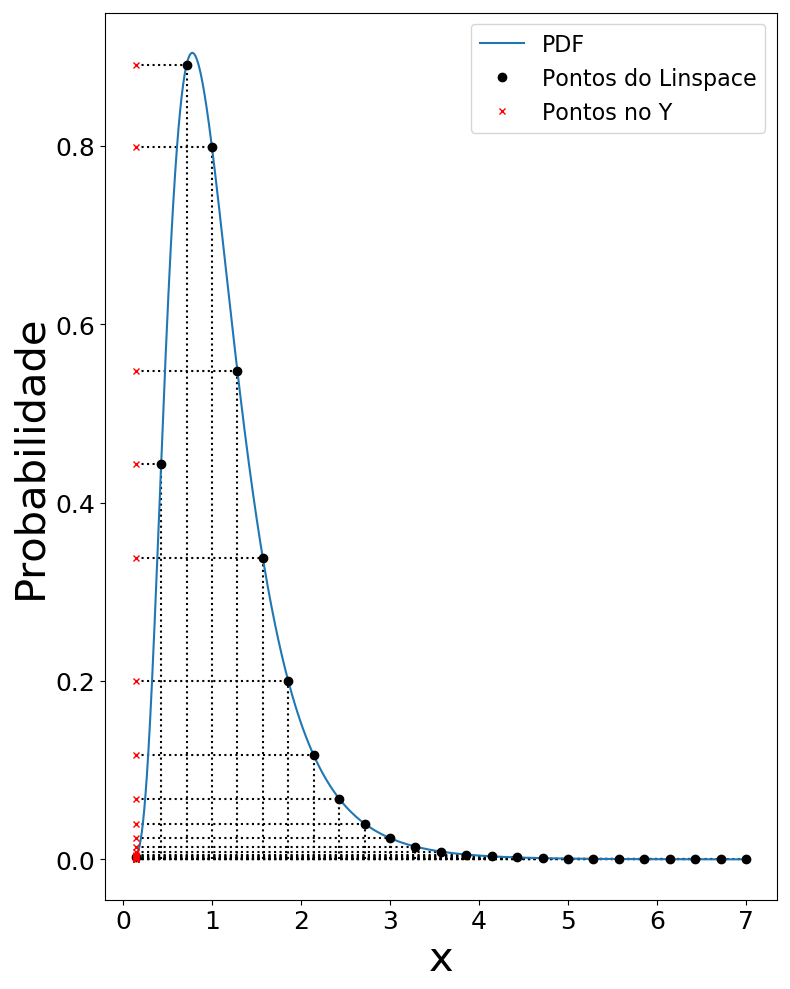
\includegraphics[width=\textwidth]{./figuras/lognormal_05}
		\caption{}
		\label{fig:lin050}
	\end{subfigure}
	
	\begin{subfigure}[b]{0.3\textwidth}
		\centering 
		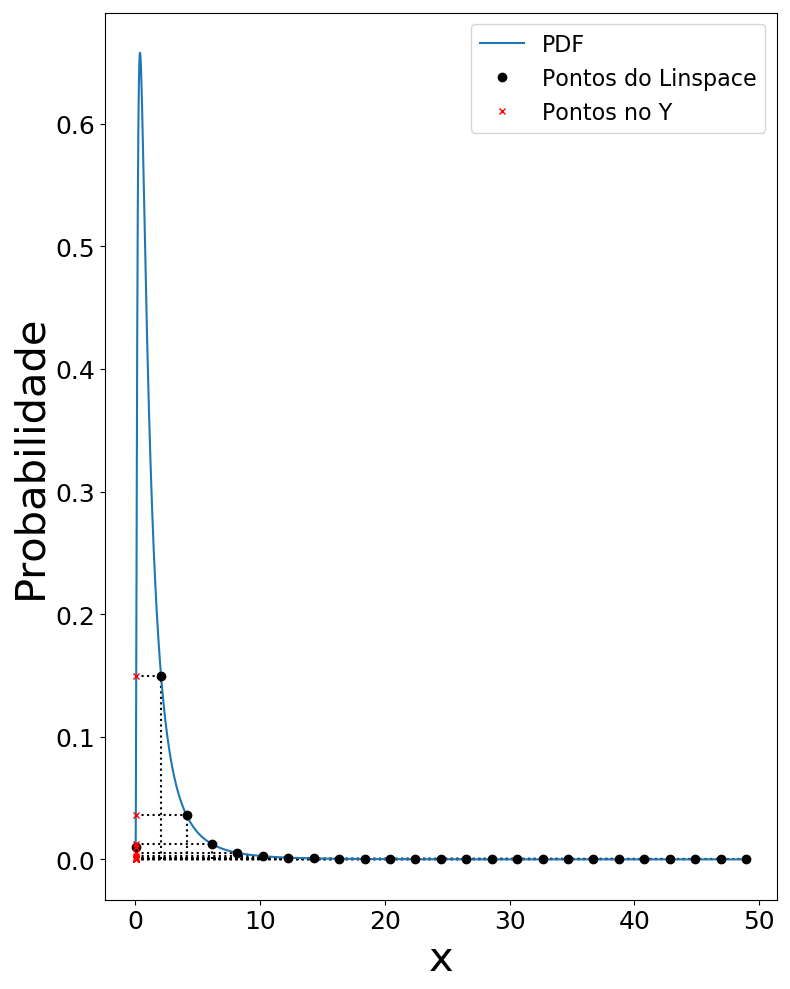
\includegraphics[width=\textwidth]{./figuras/lognormal_1}
		\caption{}
		\label{fig:lin100}
	\end{subfigure}
	\hfill
	\begin{subfigure}[b]{0.3\textwidth}
		\centering 
		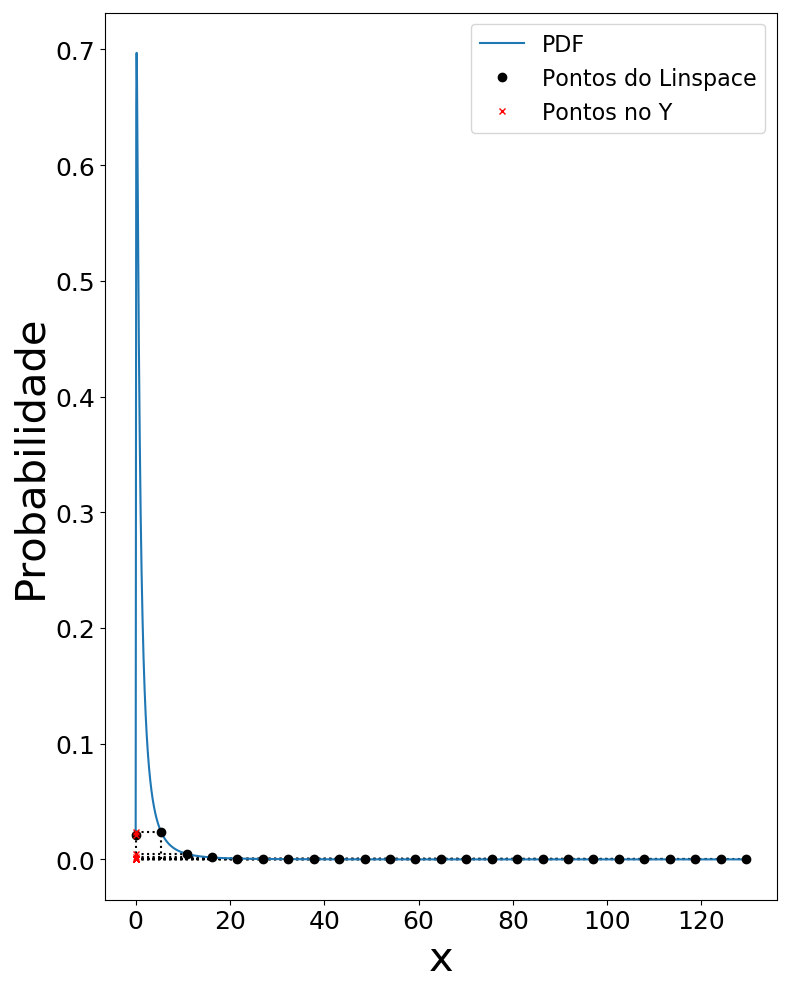
\includegraphics[width=\textwidth]{./figuras/lognormal_125}
		\caption{}
		\label{fig:lin125}
	\end{subfigure}
	\hfill
	\begin{subfigure}[b]{0.3\textwidth}
		\centering 
		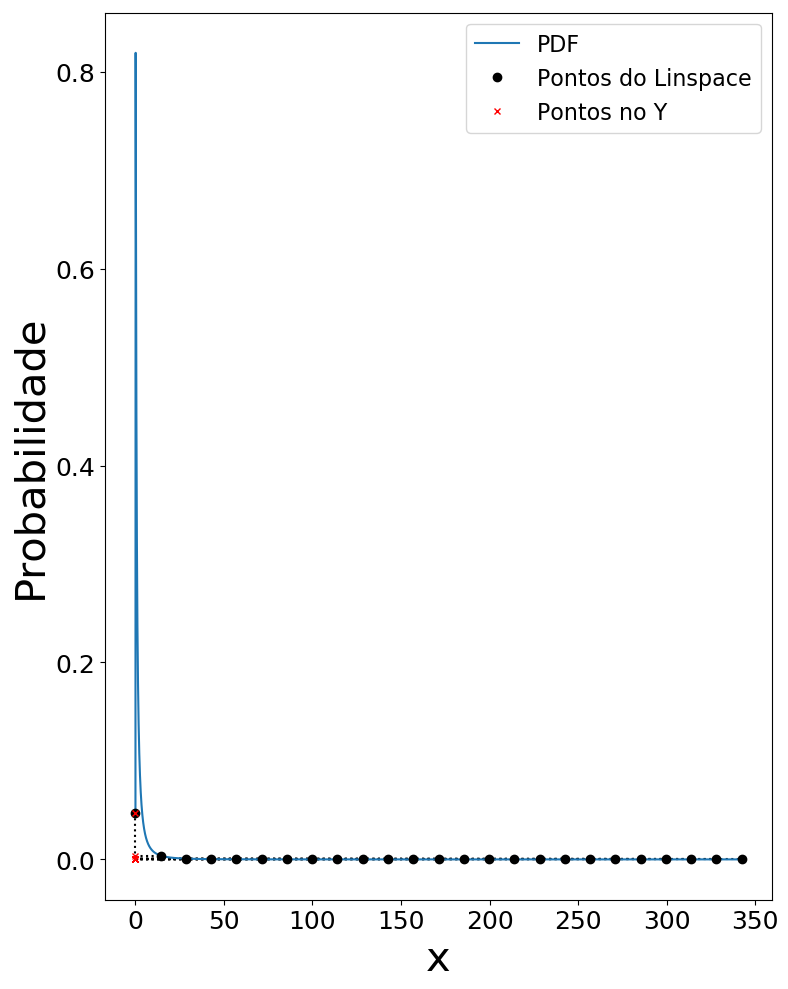
\includegraphics[width=\textwidth]{./figuras/lognormal_15}
		\caption{}
		\label{fig:lin150}
	\end{subfigure}
\caption{Ilustração do método Linspace aplicado à uma distribuição lognormal em que: (a) possui $\sigma = 0.01$; (b) possui $\sigma = 0.25$; (c) possui $\sigma = 0.5$; (d) possui $\sigma = 1$; (e) possui $\sigma = 1.25$; e (f) possui $\sigma = 1.5$}
\label{fig:Lognormal_lin}
\end{figure}


É possível perceber que este método atende de forma satisfatória distribuições que não possuem derivadas muito altas como é ilustrado na figura \ref{fig:linspace_curve} e nas figuras \ref{fig:lin001} à \ref{fig:lin050}, embora nas Figuras \ref{fig:randnlin} e \ref{fig:randloglin} há um erro de estimação por devida à quantidade de eventos simulados. Nas figuras \ref{fig:lin100} à \ref{fig:lin150} e \ref{fig:randn_outlin} o método em questão já não consegue descrever a curva, colocando um número insuficientes de pontos na região de alta probabilidade e um número superior de pontos na região de alta probabilidade.

\subsection{\textit{CDFm}}
Ela representa a discretização baseada na \ac{CDF}. Para este método, a discretização baseada no espaçamento uniforme é aplicada ao eixo vertical e então os relativos valores horizontais são encontrados refletindo todos os valores, como mostra a Figura~\ref{fig:CDFm_curve} para a distribuição Normal, a Figura~\ref{fig:Lognormal_cdf} para a distribuição Lognormal e a Figura~XXXXX para o \textit{dataset}. Note que, quanto maior a probabilidade da função de densidade, maior o número de pontos na sua região e que os \textit{outliers} não fazem mais tanto efeito, como é o cada da \textit{Linspace}.

\color{red} COLOCAR GRÁFICO 2X3 \color{black}

\begin{figure}[H]
	\centering
	\begin{subfigure}[b]{0.49\textwidth}
		\centering 
		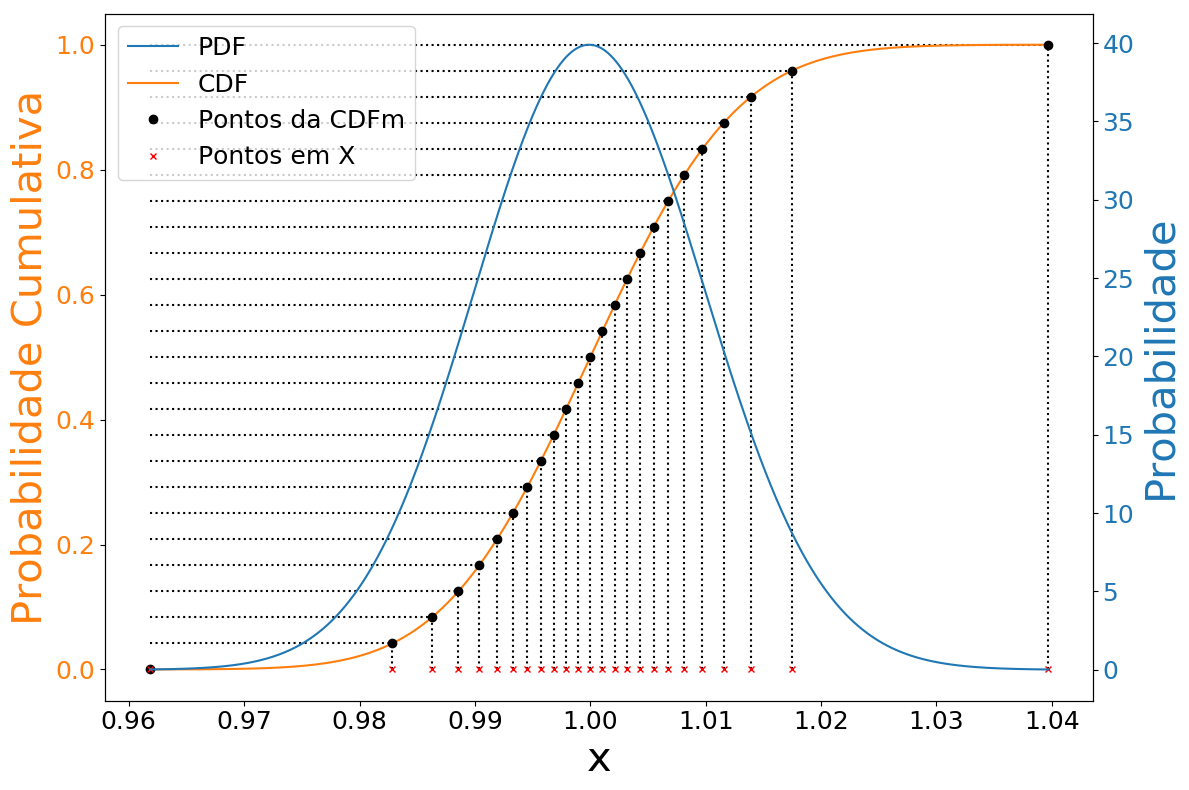
\includegraphics[width=\textwidth]{./figuras/CDFm_lognormal_001.png}
		\caption{}
		\label{fig:log001}
	\end{subfigure}
	\hfill
	\begin{subfigure}[b]{0.49\textwidth}
		\centering 
		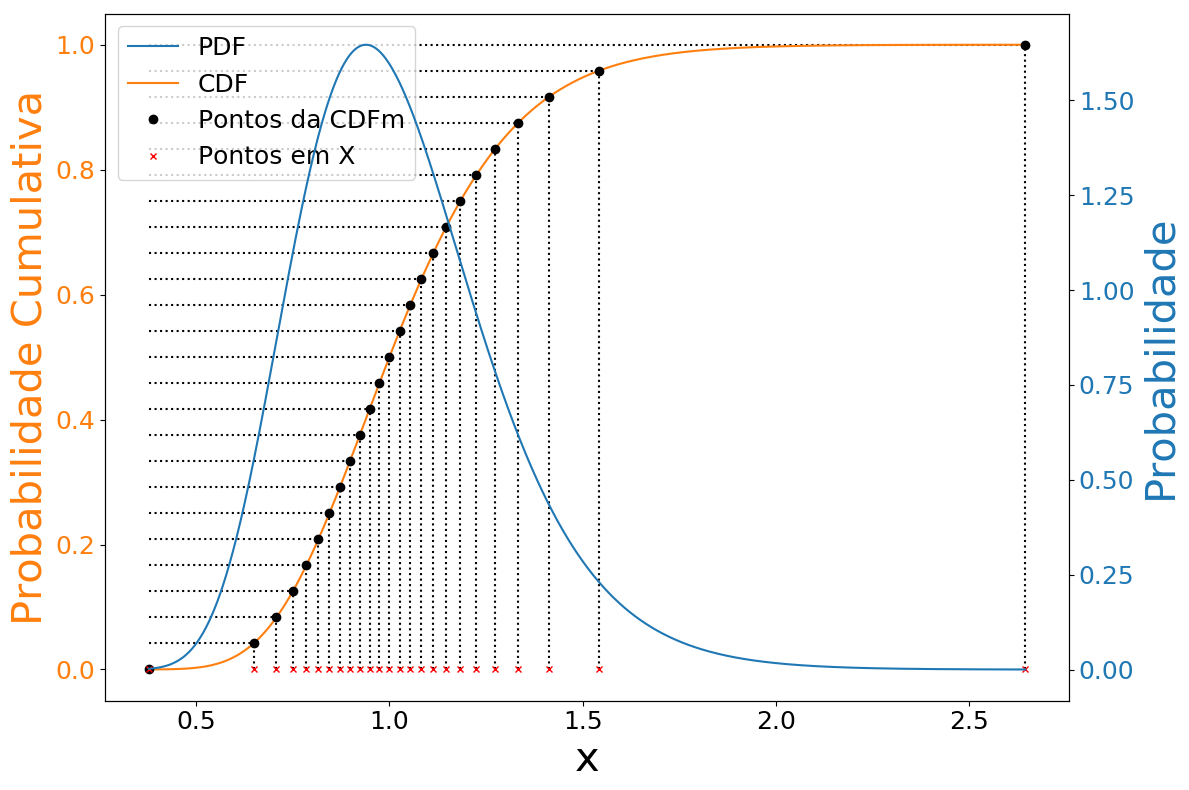
\includegraphics[width=\textwidth]{./figuras/CDFm_lognormal_025}
		\caption{}
		\label{fig:log025}
	\end{subfigure}
	
	\begin{subfigure}[b]{0.49\textwidth}
		\centering 
		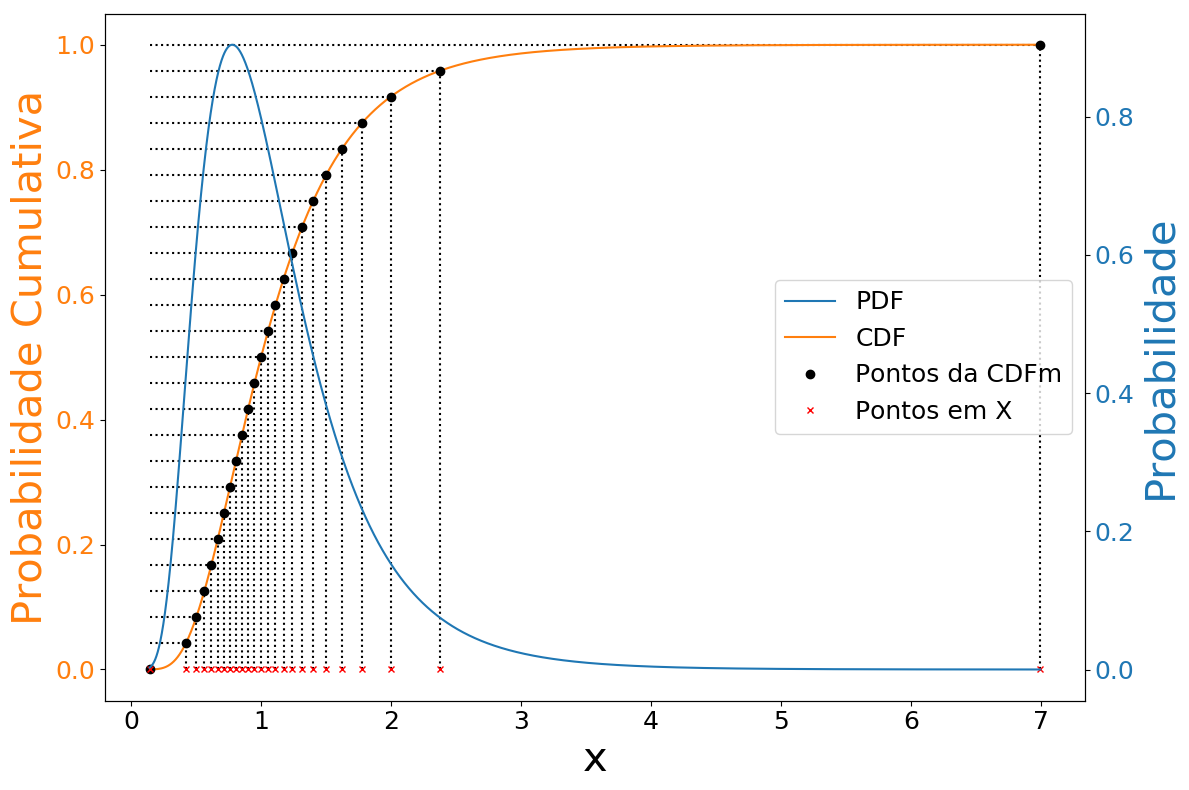
\includegraphics[width=\textwidth]{./figuras/CDFm_lognormal_05}
		\caption{}
		\label{fig:log050}
	\end{subfigure}
	\hfill
	\begin{subfigure}[b]{0.49\textwidth}
		\centering 
		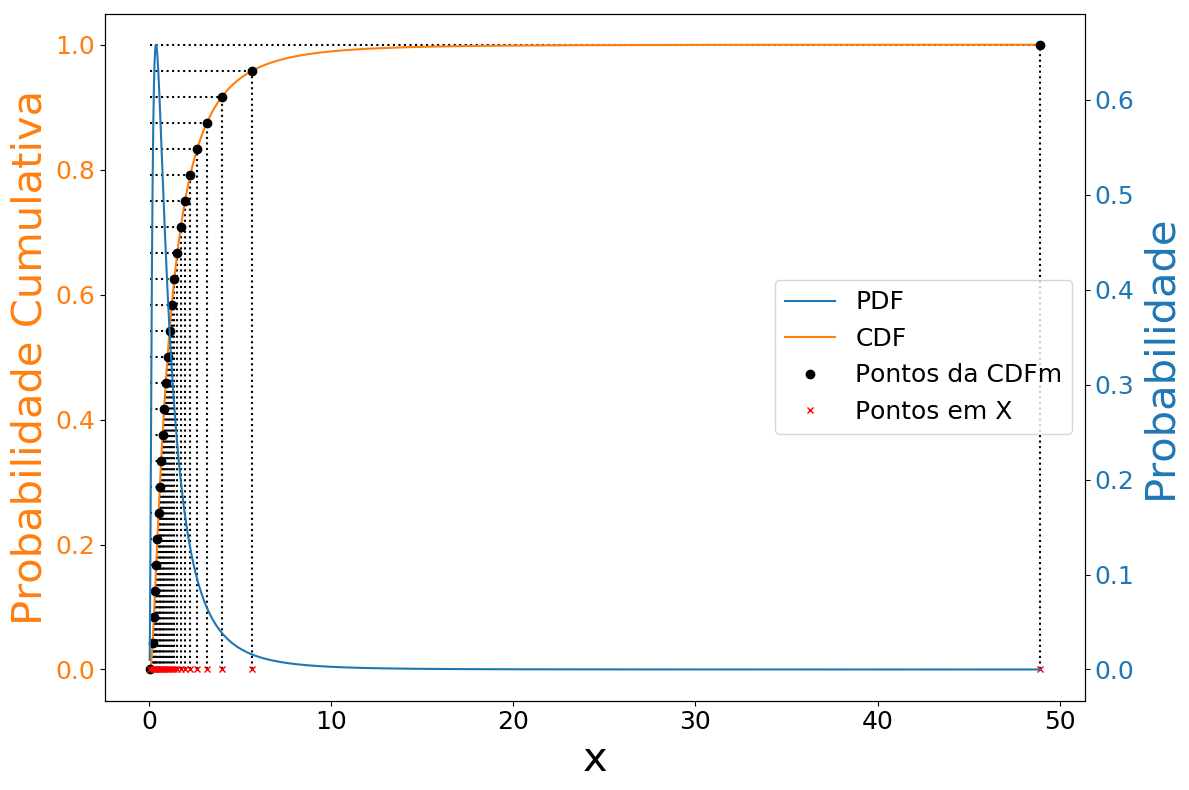
\includegraphics[width=\textwidth]{./figuras/CDFm_lognormal_1}
		\caption{}
		\label{fig:log100}
	\end{subfigure}
	
	\begin{subfigure}[b]{0.49\textwidth}
		\centering 
		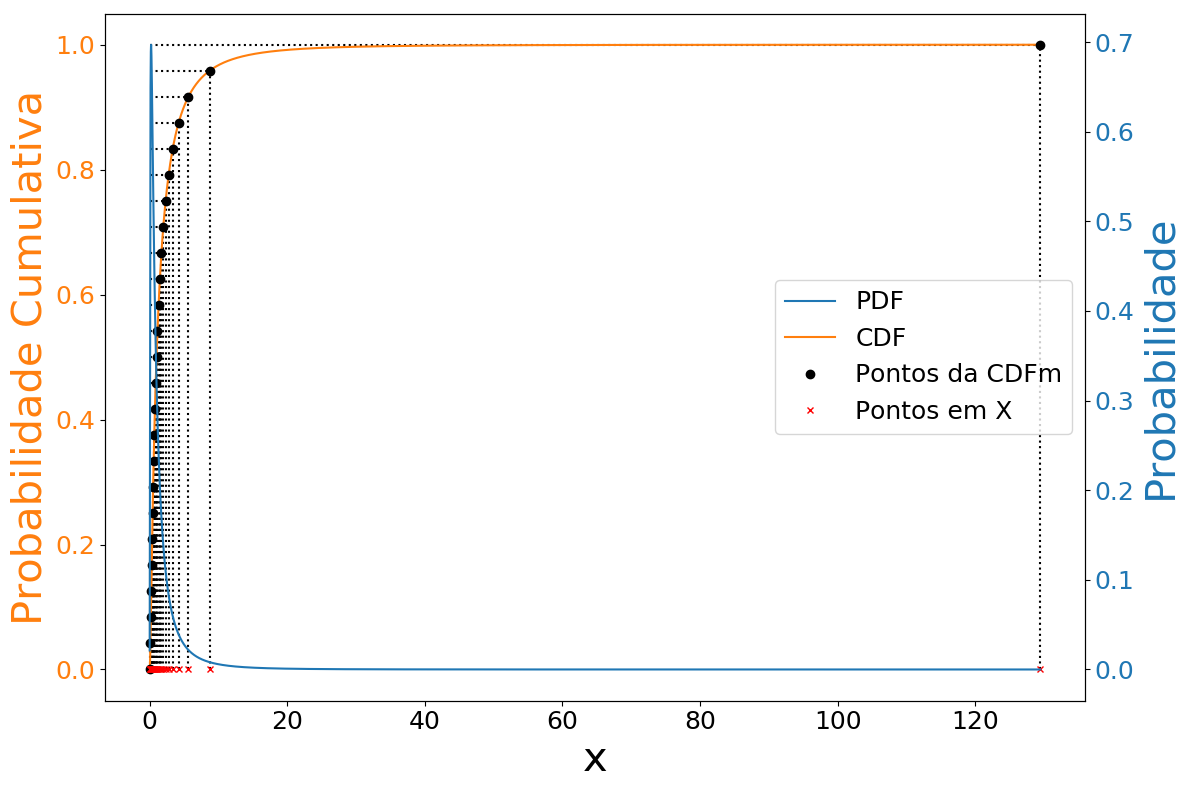
\includegraphics[width=\textwidth]{./figuras/CDFm_lognormal_125}
		\caption{}
		\label{fig:log125}
	\end{subfigure}
	\hfill
	\begin{subfigure}[b]{0.49\textwidth}
		\centering 
		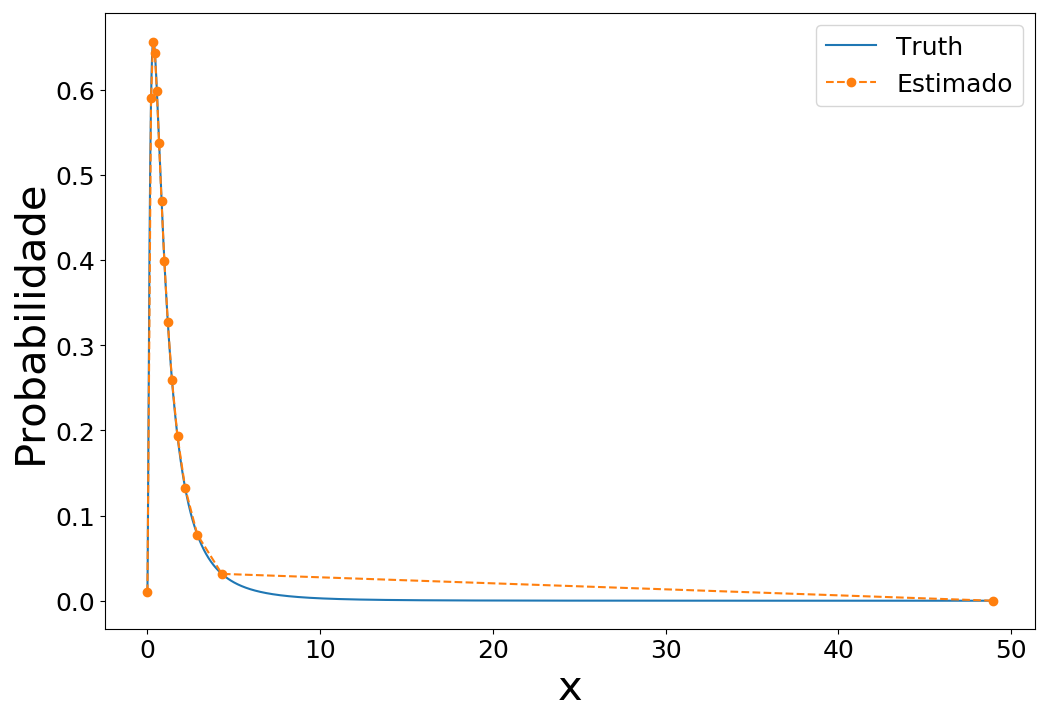
\includegraphics[width=\textwidth]{./figuras/CDFm_lognormal_15}
		\caption{}
		\label{fig:log150}
	\end{subfigure}
	\caption{Ilustração do método \textit{CDFm} aplicado à uma distribuição lognormal em que: (a) possui $\sigma = 0.01$; (b) possui $\sigma = 0.25$; (c) possui $\sigma = 0.5$; (d) possui $\sigma = 1$; (e) possui $\sigma = 1.25$; e (f) possui $\sigma = 1.5$}
	\label{fig:Lognormal_cdf}
\end{figure}

\begin{figure}[H]
	\centering
	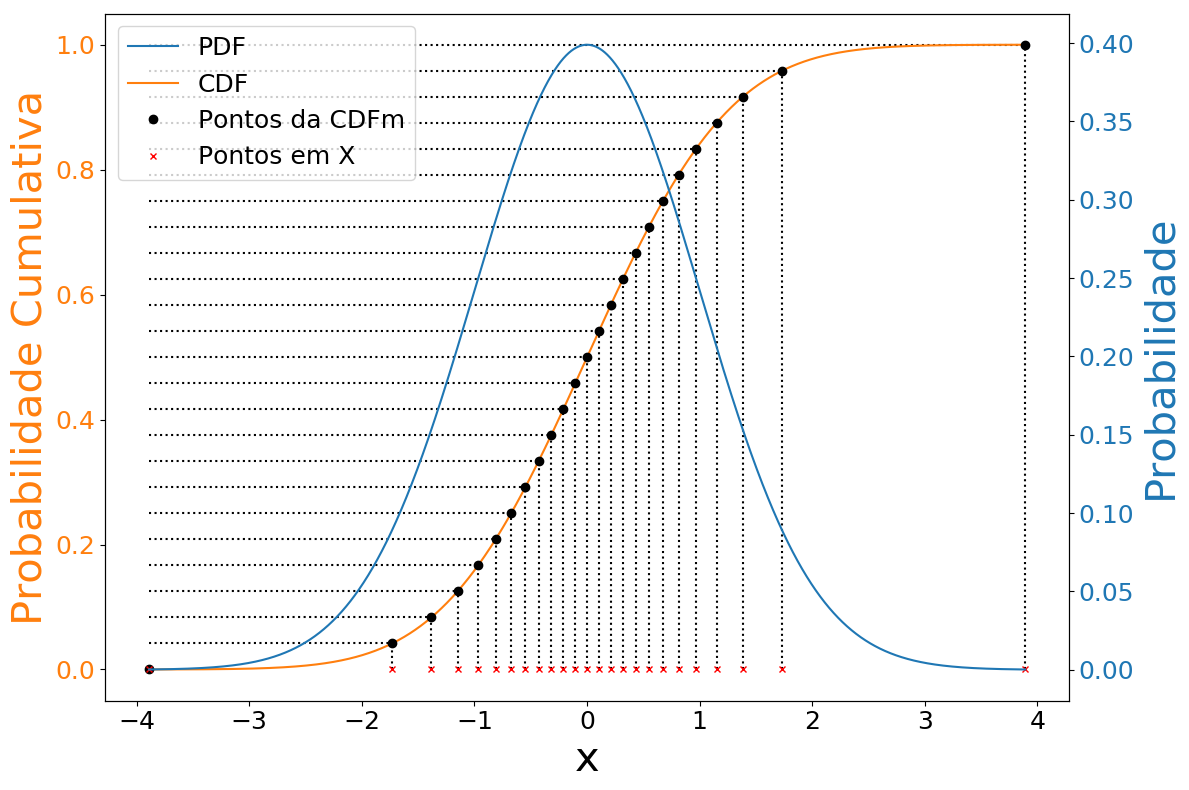
\includegraphics[width=0.8\linewidth]{./figuras/CDFm_normal_1}
	\caption{Ilustração da discretização da distribuição Gaussiana baseada em sua CDF.}
	\label{fig:CDFm_curve}
\end{figure}

\color{red} COLOCAR AQUI A FIGURA COM DATASET P/ CDFM \color{black}

Como este método baseia-se na \ac{CDF}, quando maior a variação na \ac{PDF}, mais rápido a CDF sobe, fazendo assim com que este método coloque mais pontos nas regiões de alta probabilidade e poucos pontos nas regiões de baixa probabilidade, sendo assim um método imune à \textit{outliers}.

\subsection{\textit{PDFm}}
Este método também usa a técnica de reflexão aplicada ao método da \textit{CDFm}, mas função de referência a própria \ac{PDF}, ao invés da sua \ac{CDF}. A Figura~\ref{fig:PDFm_curve} mostra como este método funciona para a distribuição Normal e a Figura~\ref{fig:Lognormal_pdf} para a distribuição Lognormal. Ela possui o efeito de incrementar o número de pontos onde a primeira derivada da \ac{PDF} é maior.

\begin{figure}[H]
	\centering
	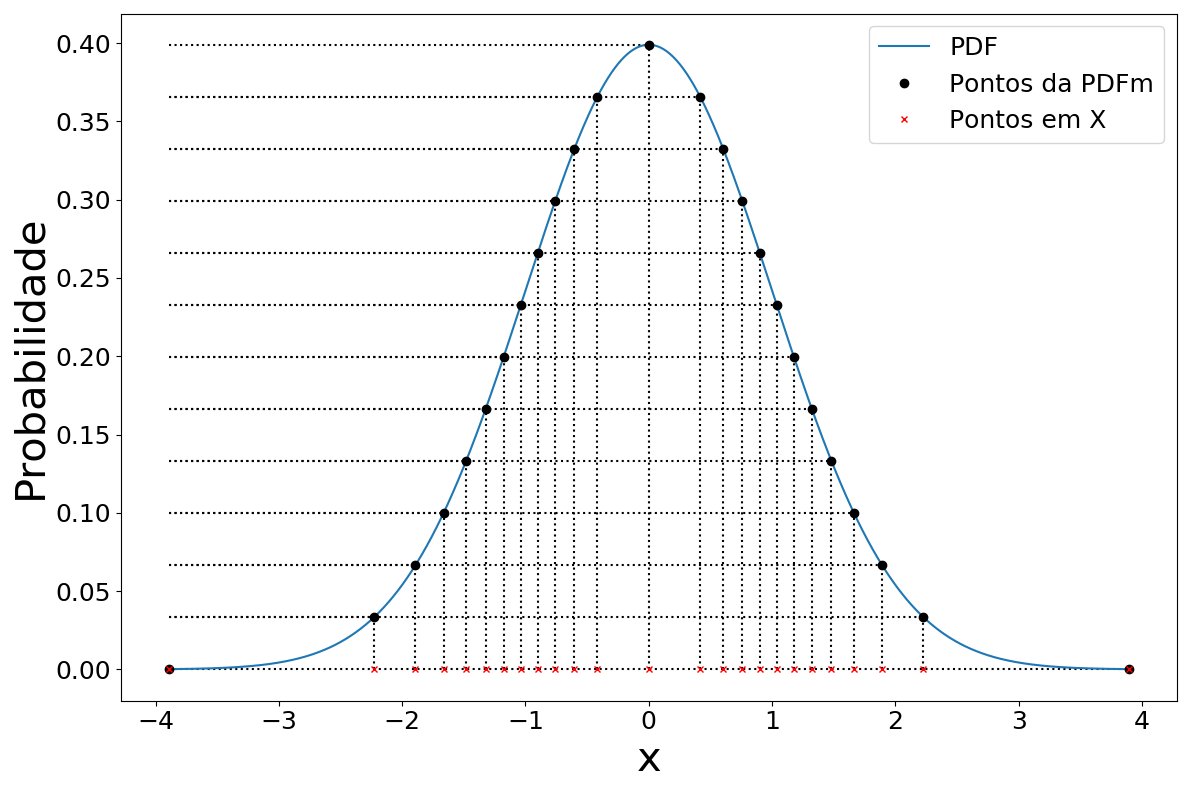
\includegraphics[width=0.67\linewidth]{./figuras/PDFm_normal_1}
	\caption{Ilustração da discretização da distribuição Gaussiana baseada em sua PDF.}
	\label{fig:PDFm_curve}
\end{figure}

{\color{red} COLOCAR GRÁFICO 2X3}

\begin{figure}[H]
	\centering
	\begin{subfigure}[b]{0.49\textwidth}
		\centering 
		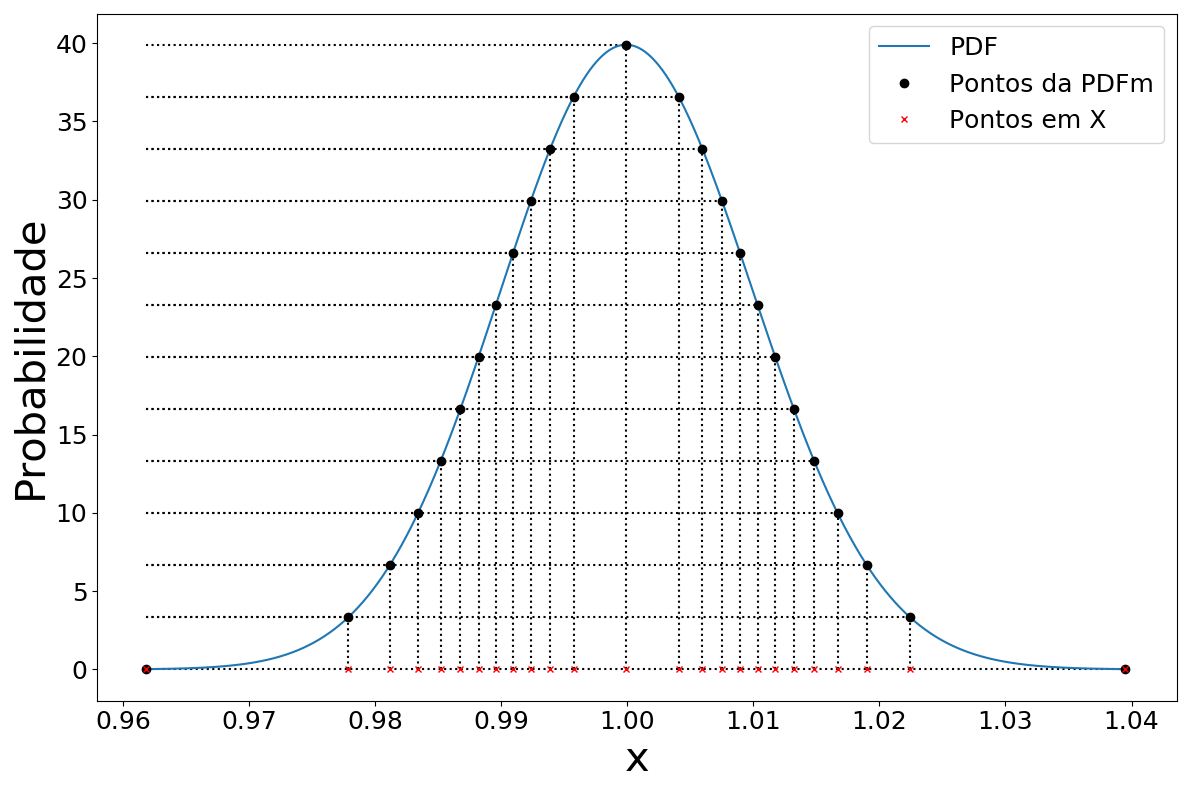
\includegraphics[width=\textwidth]{./figuras/PDFm_lognormal_001.png}
		\caption{}
		\label{fig:pdflog001}
	\end{subfigure}
	\hfill
	\begin{subfigure}[b]{0.49\textwidth}
		\centering 
		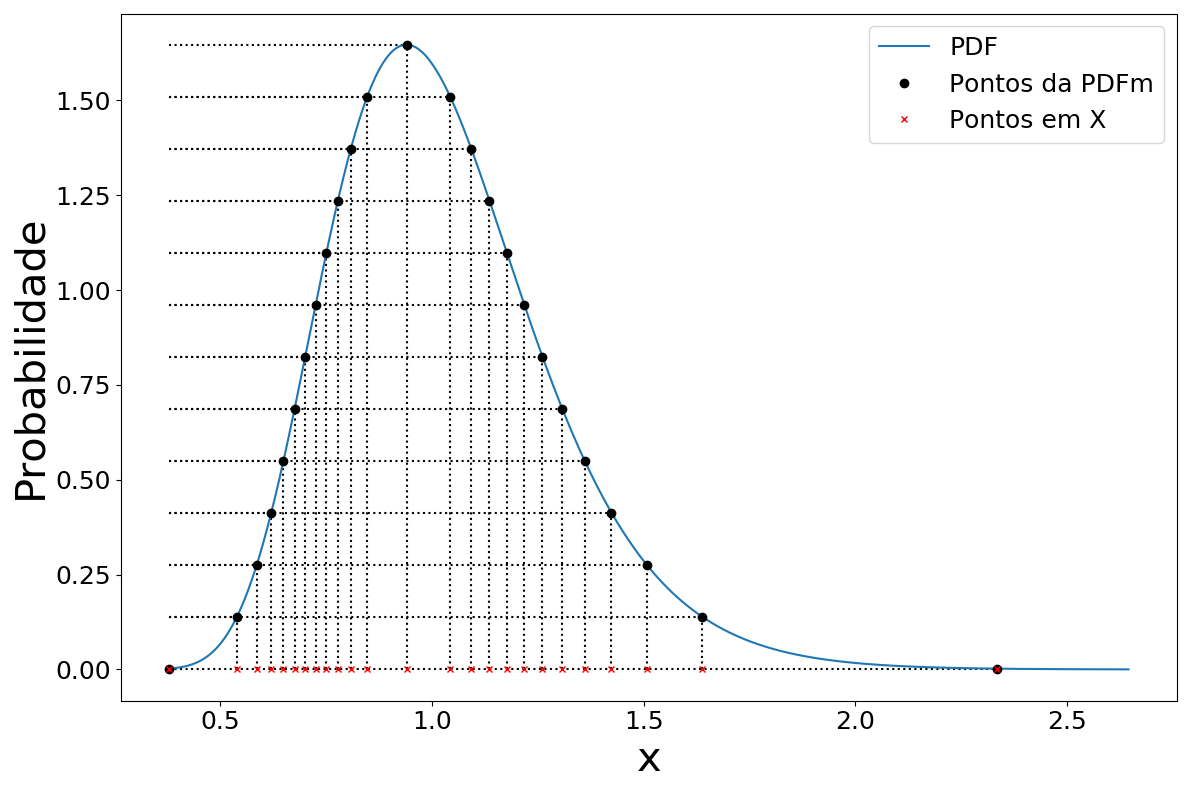
\includegraphics[width=\textwidth]{./figuras/PDFm_lognormal_025}
		\caption{}
		\label{fig:pdflog025}
	\end{subfigure}
	
	\begin{subfigure}[b]{0.49\textwidth}
		\centering 
		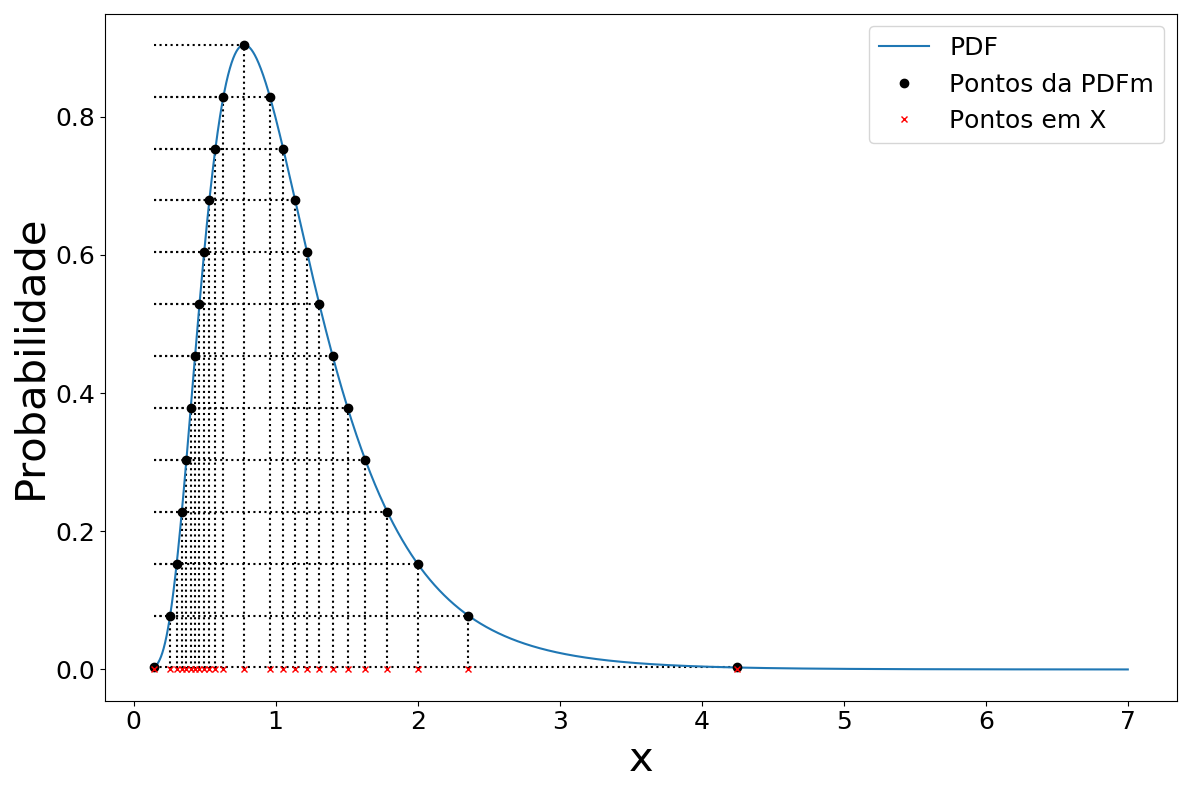
\includegraphics[width=\textwidth]{./figuras/PDFm_lognormal_05}
		\caption{}
		\label{fig:pdflog050}
	\end{subfigure}
	\hfill
	\begin{subfigure}[b]{0.49\textwidth}
		\centering 
		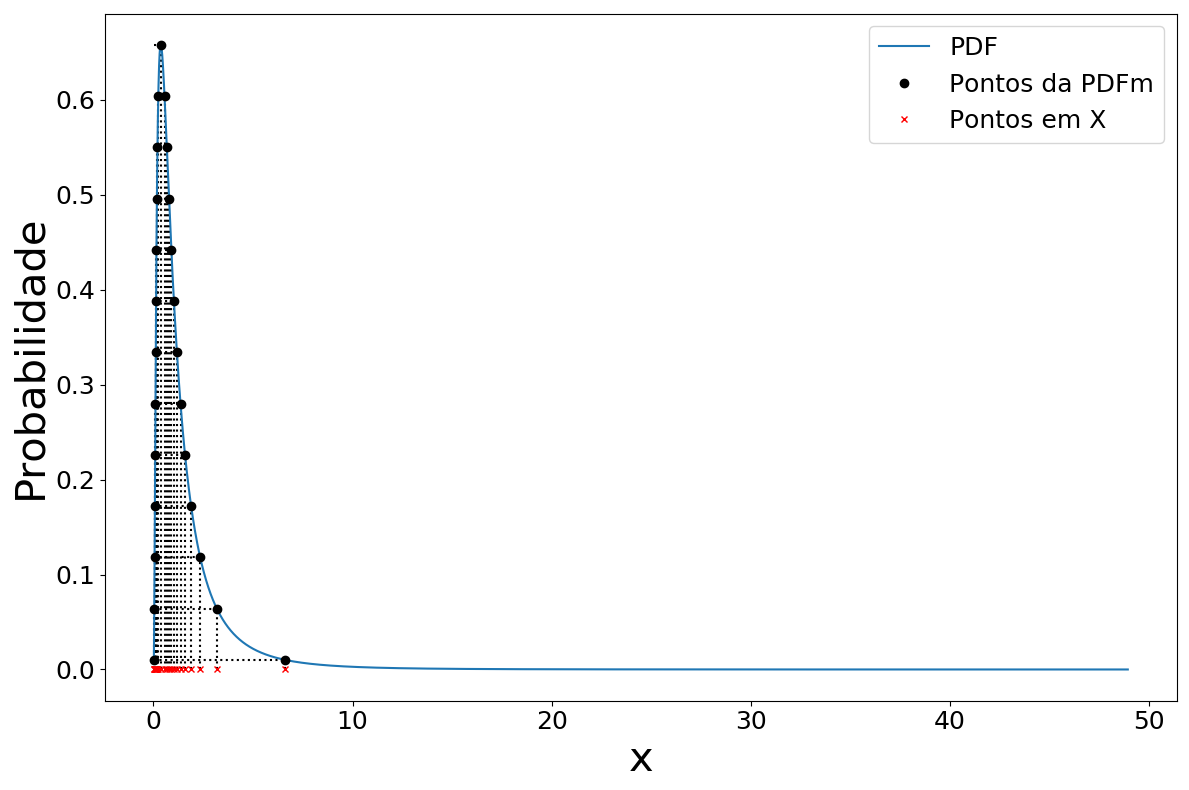
\includegraphics[width=\textwidth]{./figuras/PDFm_lognormal_1}
		\caption{}
		\label{fig:pdflog100}
	\end{subfigure}
	
	\begin{subfigure}[b]{0.49\textwidth}
		\centering 
		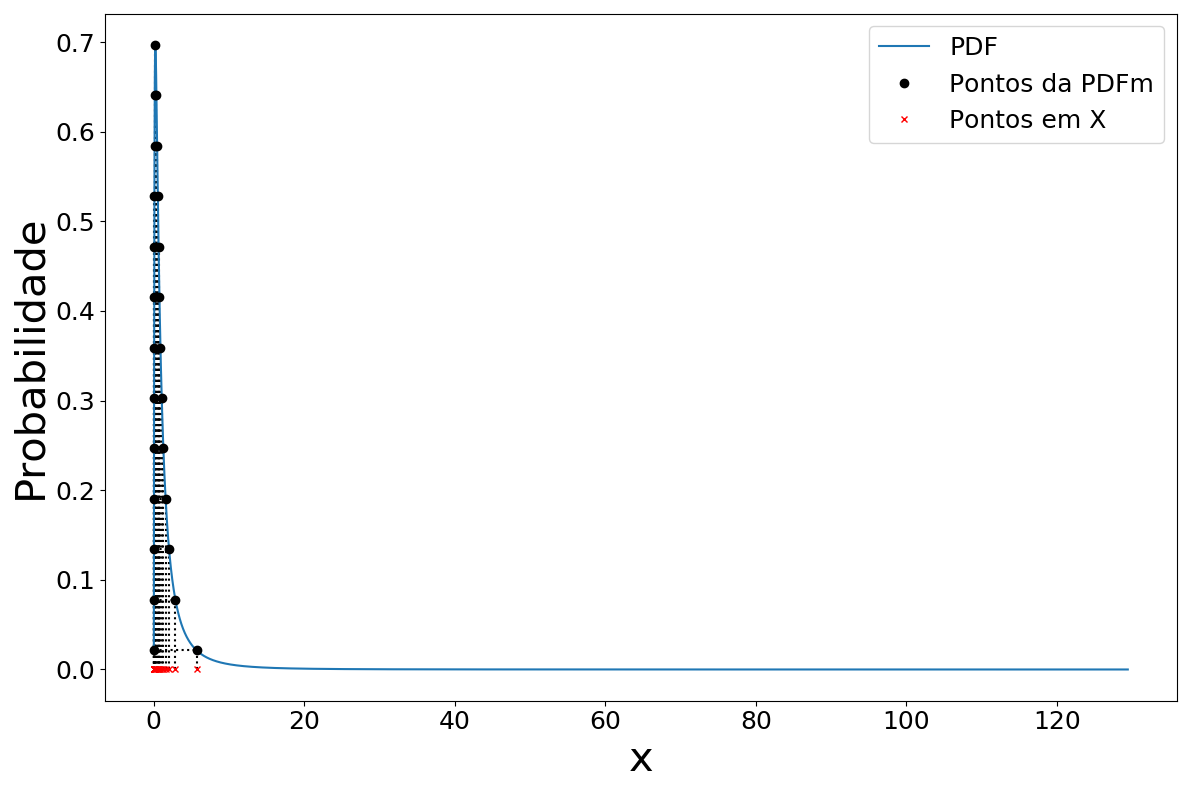
\includegraphics[width=\textwidth]{./figuras/PDFm_lognormal_125}
		\caption{}
		\label{fig:pdflog125}
	\end{subfigure}
	\hfill
	\begin{subfigure}[b]{0.49\textwidth}
		\centering 
		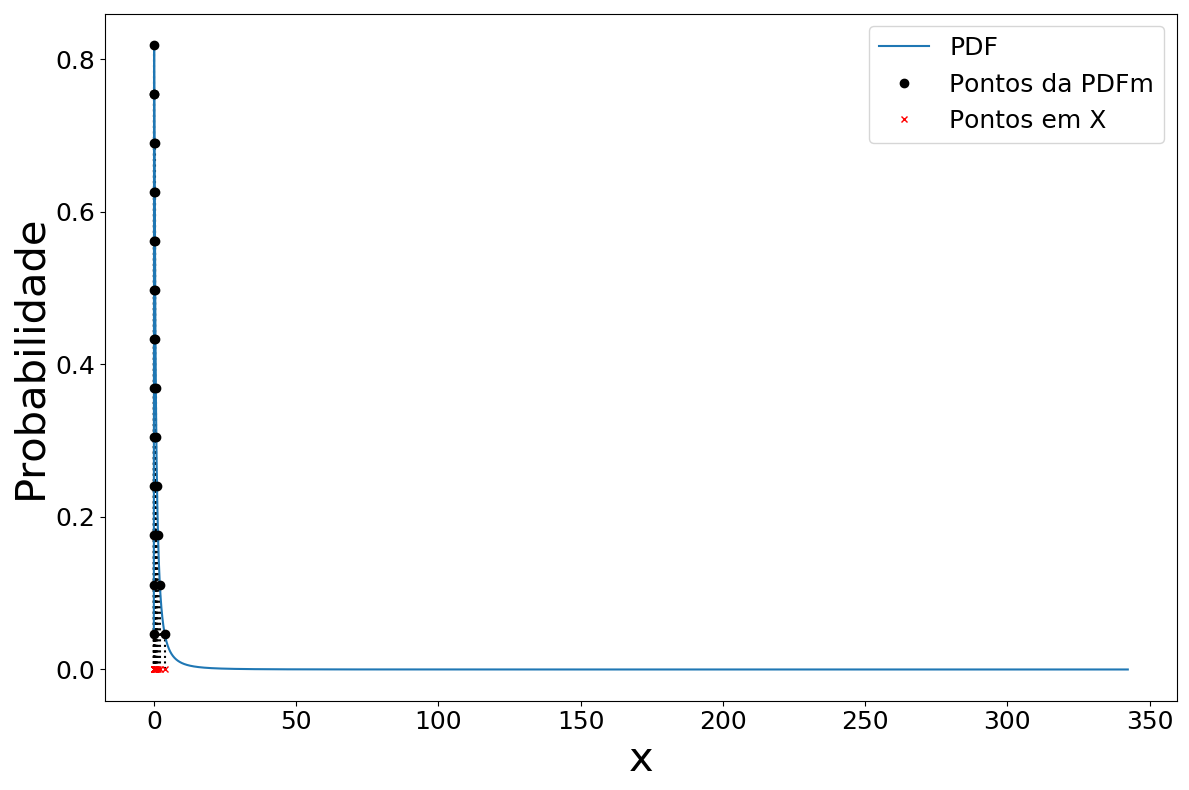
\includegraphics[width=\textwidth]{./figuras/PDFm_lognormal_15}
		\caption{}
		\label{fig:pdflog150}
	\end{subfigure}
	\caption{Ilustração do método \textit{PDFm} aplicado à uma distribuição Lognormal em que: (a) possui $\sigma = 0.01$; (b) possui $\sigma = 0.25$; (c) possui $\sigma = 0.5$; (d) possui $\sigma = 1$; (e) possui $\sigma = 1.25$; e (f) possui $\sigma = 1.5$}
	\label{fig:Lognormal_pdf}
\end{figure}

{\color{red} COLOCAR GRÁFICO DOS DATASETS}

\subsection{\textit{iPDF1}}

Este método reflete os valores verticais para o eixo horizontal usando a \ac{CDF} da primeira derivada da \ac{PDF} como uma transformação de base, como é ilustrado nas Figuras~\ref{fig:dPDF1} e \ref{fig:dPDF2}
{\color{red} COLOCAR O GRÁFICO DA DERIVADA EM ANEXO E AQUI O GRÁFICO DA CDF PARA A LOGNORMAL E COM OS DATASETS}
\begin{figure}[!ht]
	\centering
	\begin{subfigure}[b]{0.44\textwidth}
		\centering 
		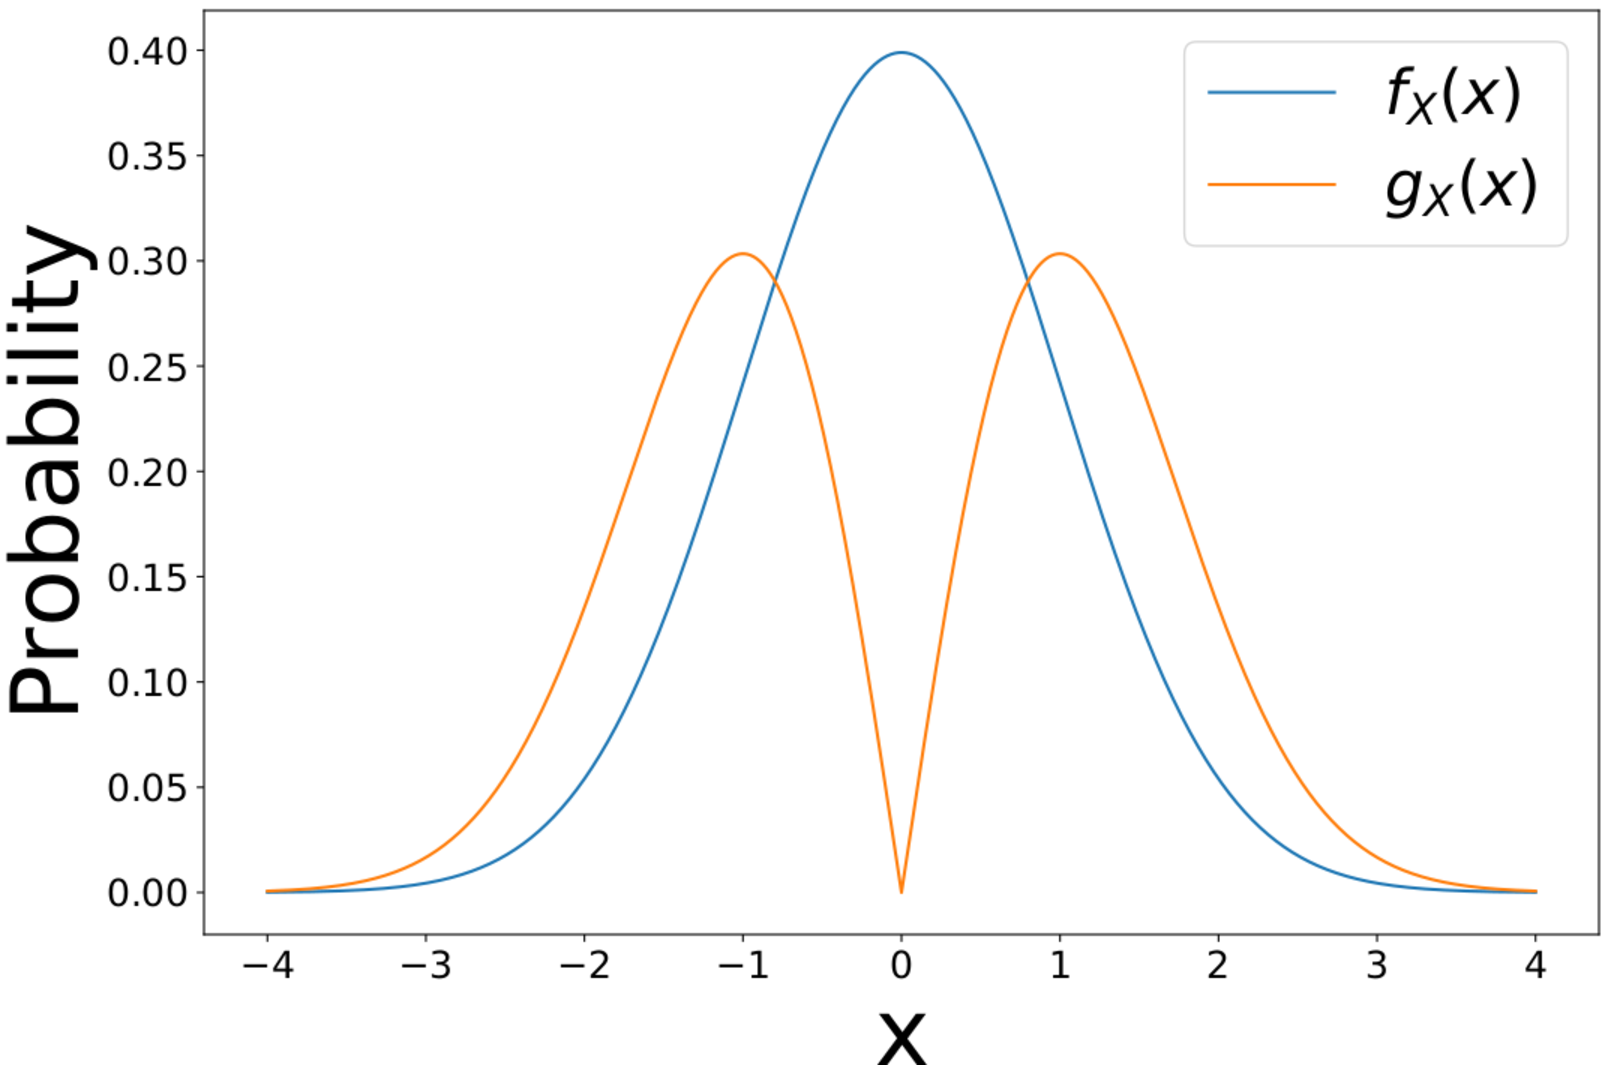
\includegraphics[width=\textwidth]{./figuras/dpdf1}
		\caption{}
		\label{fig:dPDF1}
	\end{subfigure}
	\hfill
	\begin{subfigure}[b]{0.47\textwidth}
		\centering 
		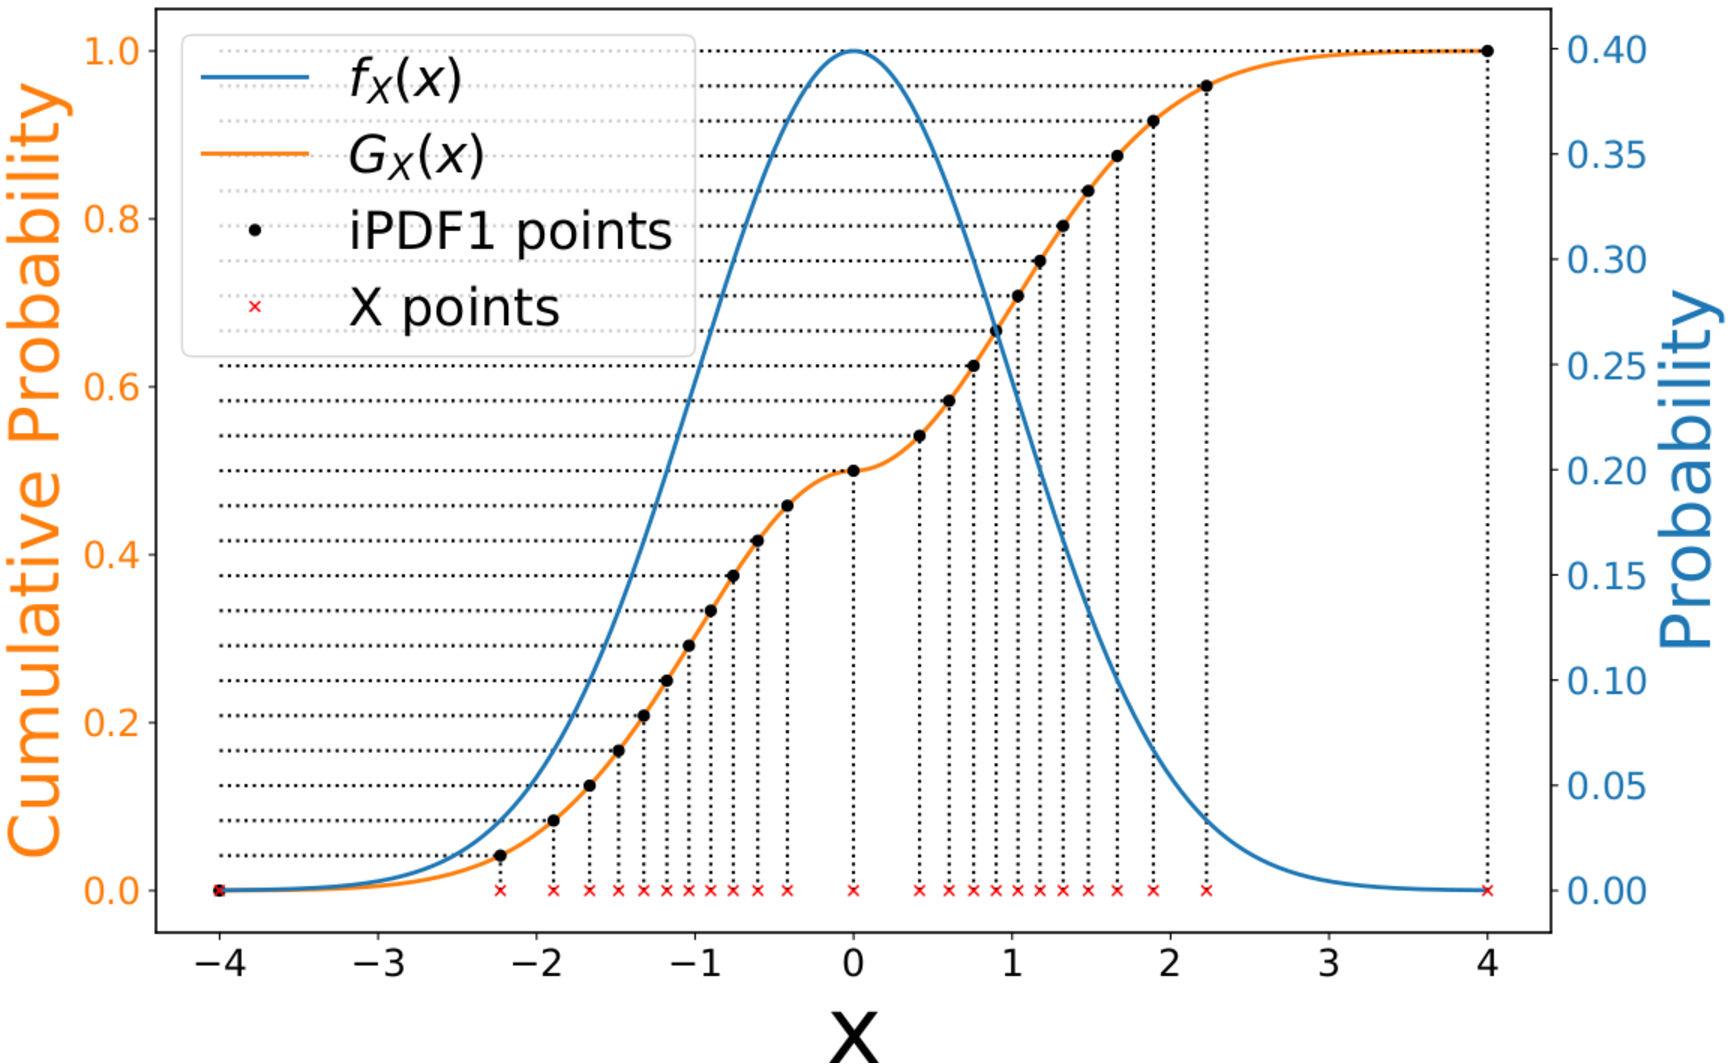
\includegraphics[width=\textwidth]{./figuras/dpdf2}
		\caption{}
		\label{fig:dPDF2}
	\end{subfigure}
\caption{PDF Gaussiana e sua primeira derivada à esquerda. Ilustração da discretização da distribuição Gaussiana baseada na CDF da sua primeira derivada à direita.}
\label{fig:dPDF}
\end{figure}

As equações \eqref{equ:dpdf1} e \eqref{equ:dcdf} descrevem este método matematicamente.

\color{red} COLOCAR AQUI TB A EQUAÇÃO PRA LOGNORMAL \color{black}
\begin{equation}
\begin{array}{l}
\vspace{0.3cm}\displaystyle \zeta(x) = \frac{|\mu-x|}{\sigma^3\sqrt{2\pi}}\cdot e^{\left(\frac{-(\mu-x)^2}{2\sigma^2}\right) } \\
\vspace{0.3cm} \displaystyle \int_{-\infty}^{\infty} \zeta(x)\cdot dx = c_1 \\
\displaystyle g_X(x) = \frac{\zeta(x)}{c_1}
\label{equ:dpdf1}
\end{array}
\end{equation}
onde $\zeta$ é a equação da distribuição da derivada da distribuição normal, $\mu$ é a média, $\sigma$ o desvio padrão, $x$ a variável aleatória, $c_1$ é a área abaixo da curva $\zeta$, e $g_X$ é a versão normalizada.	
A \ac{CDF} de $g_X$ ($G_X(x)$) é usada para transferir os valores da abscissa ao eixo da ordenada como mostra a  Figura~\ref{fig:dPDF2}.

\begin{equation}
G_X(x) = \int_{-\infty}^x g_X(y)\cdot dy
\label{equ:dcdf}
\end{equation}

\subsection{\textit{iPDF2}}
Este método é construído da mesma maneira da \textit{IPDF1} mas usando a segunda detivada ao invés da primeira, como é mostrado na Figura~\ref{fig:ddPDF1} e \ref{fig:ddPDF2}. Suas equações são mostradas em \eqref{equ:hx} e \eqref{equ:ddcdf}.

{\color{red} COLOCAR O GRÁFICO DA DERIVADA EM ANEXO E AQUI O GRÁFICO DA CDF PARA A LOGNORMAL E COM OS DATASETS}

\begin{figure}[ht]
	\centering
	\begin{subfigure}[b]{0.44\textwidth}
		\centering 
		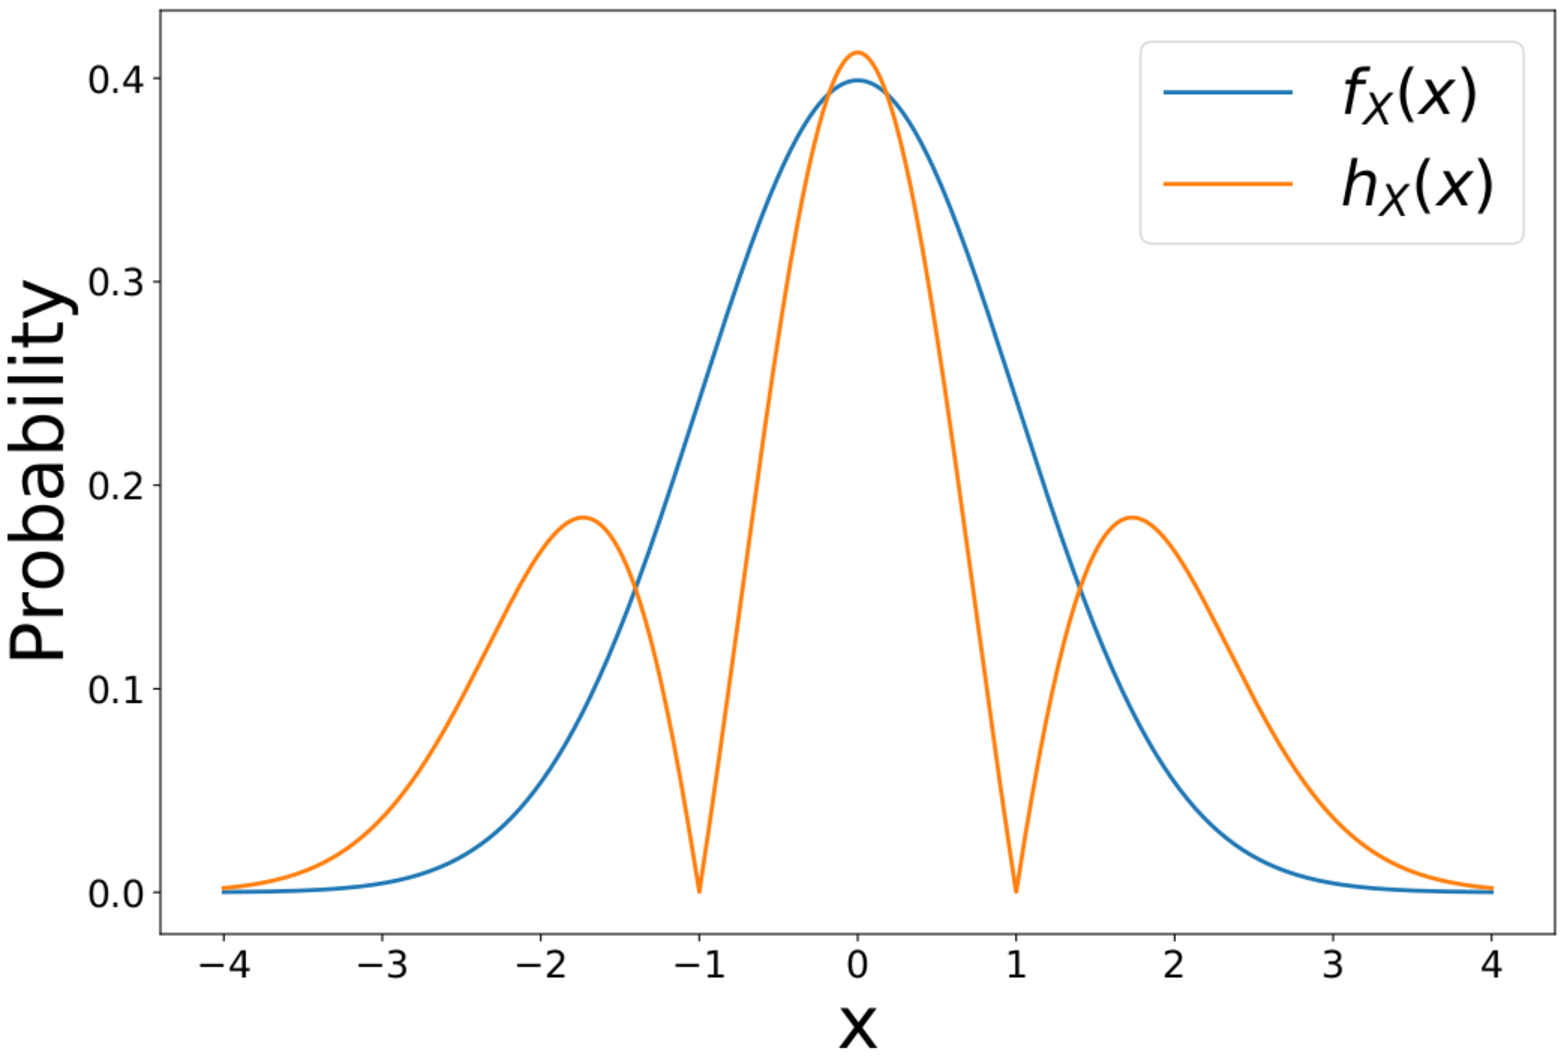
\includegraphics[width=\textwidth]{./figuras/ddpdf1.pdf}
		\caption{}
		\label{fig:ddPDF1}
	\end{subfigure}
	\hfill
	~ %add desired spacing between images, e. g. ~, \quad, \qquad, \hfill etc. 
	%(or a blank line to force the subfigure onto a new line)
	\begin{subfigure}[b]{0.47\textwidth}
		\centering 
		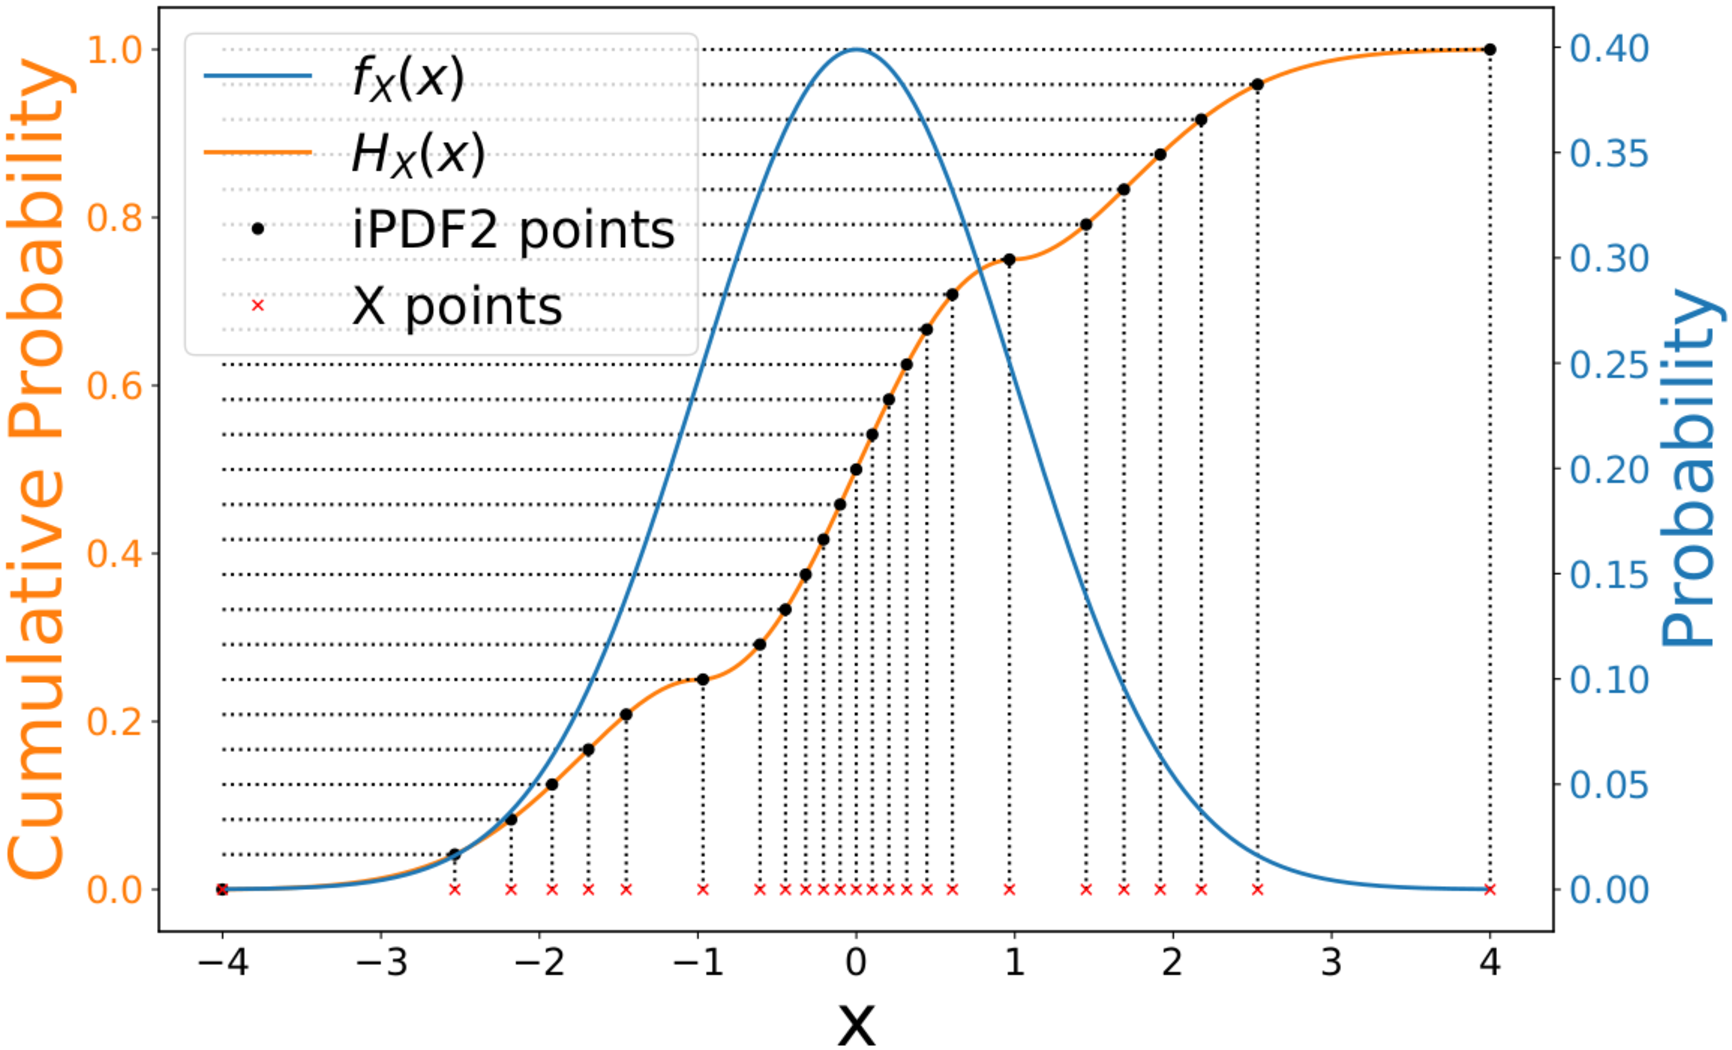
\includegraphics[width=\textwidth]{./figuras/ddpdf2.pdf}
		\caption{}
		\label{fig:ddPDF2}
	\end{subfigure}
	
	\caption{PDF Gaussiana e sua segunda derivada à esquerda. Ilustração da discretização da distribuição Gaussiana baseada na CDF da sua segunda derivada à direita.}
	\label{fig:ddPDF}
\end{figure}
\color{red} COLOCAR AQUI TB A EQUAÇÃO PRA LOGNORMAL \color{black}
\begin{equation}
\begin{array}{l}
\vspace{0.3cm}\displaystyle \eta(x) = \frac{|\sigma^2 - (\mu - x)^2|}{ \sigma^5\sqrt{2\pi}}\cdot e^{-\frac{(\mu - x)^2}{2 \sigma^2}} \\
\vspace{0.3cm} \displaystyle \int_{-\infty}^{\infty} \eta(x)\cdot dx = c_2 \\
\displaystyle h_X(x) = \frac{\eta(x)}{c_2}
\label{equ:hx}
\end{array}
\end{equation}
onde $\eta$ é a equação de distribuição de segunda derivada da distribuição Normal, $c_2$ é a área abaixo da curva desta distribuição, e $h_X$ é sua versão normalizada. 
Finalmente, $H_X(x)$ é a \ac{CDF} de $h_X$, dada por \eqref{equ:ddcdf}.

\begin{equation}
H_X(x) = \int_{-\infty}^x h_X(y)\cdot dy
\label{equ:ddcdf}
\end{equation}


\section{Ambiente de Análise}
Para analisar as diferenças entre a \ac{PDF} real e estimada ao longo de toda a extensão do eixo das abscissas, a área entre as duas \ac{PDF}s será usada como medida da estimação de erro. Além do mais, o eixo das abscissas foi dividida em $N$ regiões de mesmo tamanho, chamado \ac{RoI} \cite{ron1999art}. Essas regiões são compreendidas entre valores máximos e mínimos predefinidos do eixo horizontal. A Figura~XXXXX mostra este processo quando a abscissa é dividida em 20 regiões, todas compreendidas entre os valores $-4$ e $4$ do eixo $ x $.


{\color{red} COLOCAR AQUI O GRÁFICO COM O ERRO QUE TEM ZOOM}

A maneira que a \ac{RoI} é usada neste trabalho permitirá avaliar o erro de estimação em função de quatro diferentes parâmetros: Probabilidade; Eixo das abscissas; Primeira e Segunda Derivada. Para estimar os valores entre os pontos discretos, dois métodos de interpolação serão usados: interpolação pelo Vizinho Mais Próximo e Linear. 200 amostras serão usadas no processo de discretização. O erro de estimação tende a melhoras conforme o número de amostras aumenta mas sua característica geral não muda. Este último é a principal preocupação deste trabalho.


\chapter{RESULTADOS} \label{cap:resultados}
\vspace{-2cm}
Nessa seção os resultados serão dados em termos da área medida entre a diferença da \ac{PDF} real e a estimada, como previamente mencionado. Nas figuras que seguem, esses valores serão mostrados no eixo vertical, nomeado de \textit{Erro}. O eixo horizontal mostra quatro perspectivas diferentes: Probabilidade, Eixo $ x $ (que seria os valores aleatórios da variável), Primeira derivada, e Segunda derivada. Além disso há outra figura que mostra como o método se comporta quando o número de pontos de estimação varia sendo que, para os dados gerados, foram pegos 10 amostras que são representadas com a sua média e seu erro como o desvio padrão dessa média sobre a raiz quadrada do número de amostras. Essas perspectivas diferentes irão permitir um melhor entendimento das características de cada método. Essa sessão será dividida em três análises diferentes. Sessão~\ref{cap:interp_neares} analisa a estimação de erro quando a interpolação pelo vizinho mais próximo é usada; Sessão~\ref{cap:interp_lin} avalia para a interpolação linear; e a Sessão~\ref{cap:erro_out} insere problemas de \textit{outliers}. Quando \textit{outliers} são gerados, o desempenho de alguns métodos de discretização podem ser altamente degradados em comparação com outros, sendo uma questão importante a ser analisada.

\section{Estimação de erro pela interpolação do vizinho mais próximo} \label{cap:interp_neares}
A interpolação pelo vizinho mais próximo basicamente atribui o valor conhecido mais próximo ao valor da probabilidade da variável aleatória que será estimada. Portanto, o erro de estimação será proporcional à sua distância da amostra mais próxima. Tal método de interpolação produz um erro diretamente proporcional à primeira derivada \cite{gurevich1966integral}. A Figura \ref{fig:12} mostra essa análise para a distribuição normal enquanto a Figura~\ref{fig:error_lognormal_nearest} mostra o comportamento para a distribuição Lognormal.  

\begin{figure}[H]
	\centering
	\begin{subfigure}[b]{0.45\textwidth}
		\centering 
		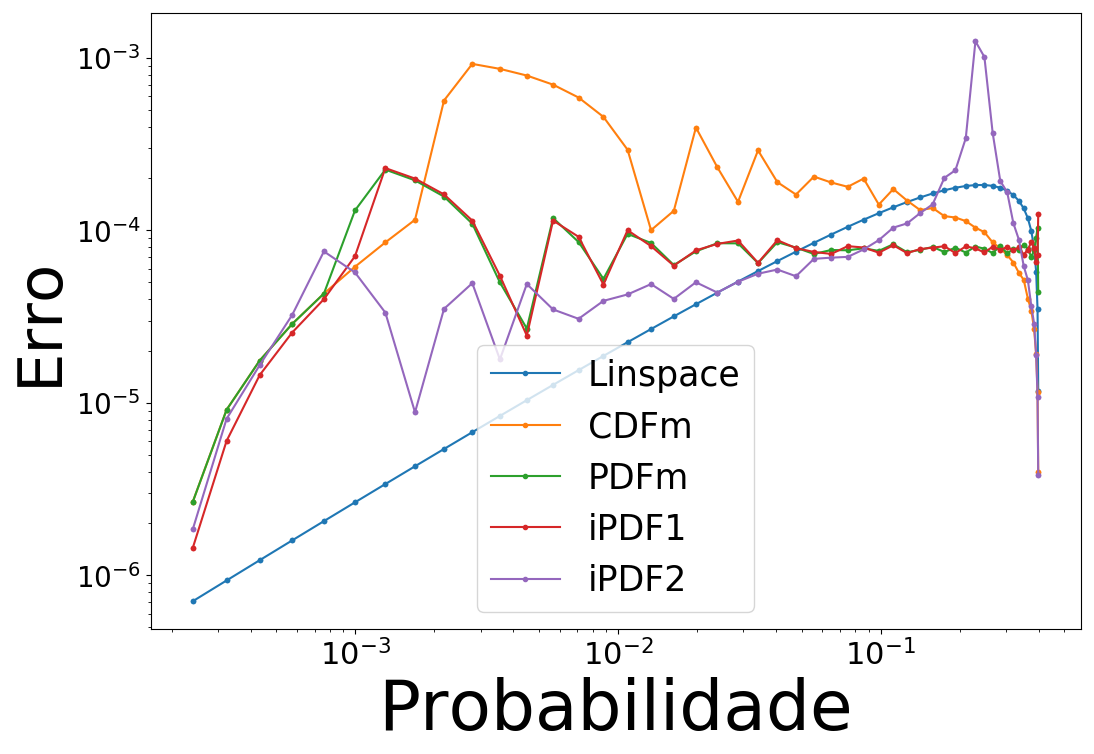
\includegraphics[width=\textwidth]{./figuras/error_normal_nearest_Probabilidade_1}
		\caption{}
		\label{fig:12a}
	\end{subfigure}
	\hfill
	~ %add desired spacing between images, e. g. ~, \quad, \qquad, \hfill etc. 
	%(or a blank line to force the subfigure onto a new line)
	\begin{subfigure}[b]{0.45\textwidth}
		\centering 
		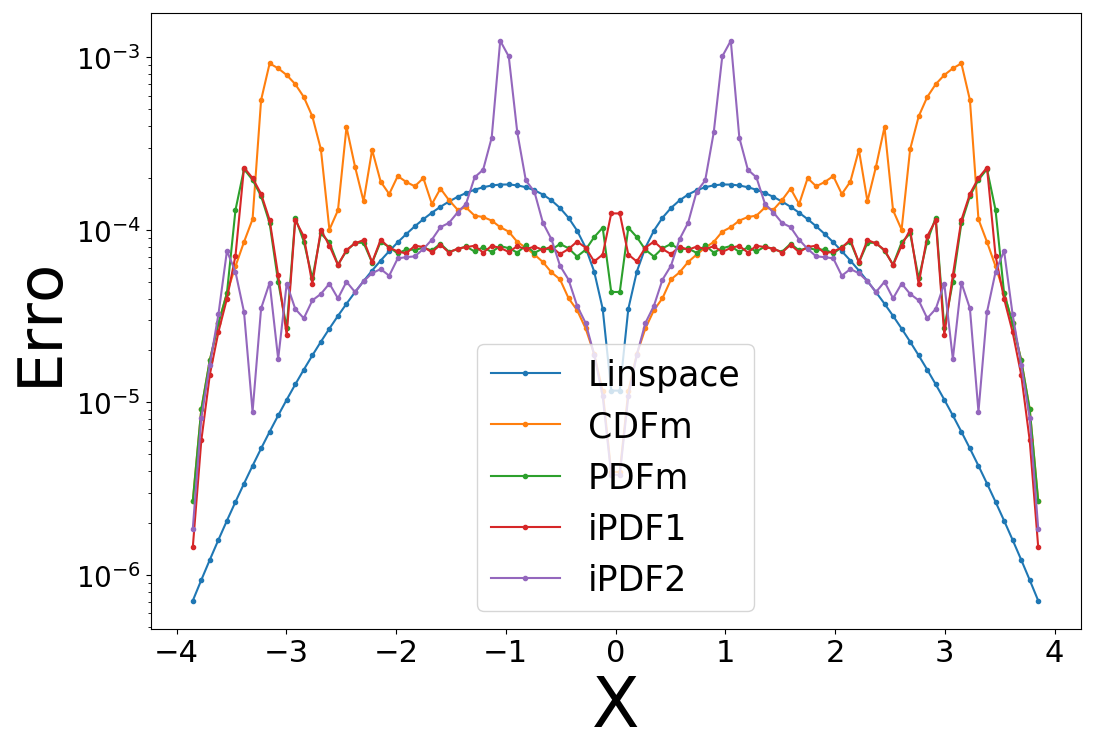
\includegraphics[width=\textwidth]{./figuras/error_normal_nearest_X_1}
		\caption{}
		\label{fig:12b}
	\end{subfigure}
	%\vskip\baselineskip
	~ %add desired spacing between images, e. g. ~, \quad, \qquad, \hfill etc. 
	%(or a blank line to force the subfigure onto a new line)
	\begin{subfigure}[b]{0.45\textwidth}
		\centering 
		\includegraphics[width=\textwidth]{./figuras/error_normal_nearest_Primeira_Derivada_1.png}
		\caption{}
		\label{fig:12c}
	\end{subfigure}
	\hfill
	\begin{subfigure}[b]{0.45\textwidth}
		\centering 
		\includegraphics[width=\textwidth]{./figuras/error_normal_nearest_Segunda_Derivada_1.png}
		\caption{}
		\label{fig:12d}
	\end{subfigure}
	\caption{Caso representativo da distribuição Gaussiana com 200 pontos, 100 RoIs e usando a interpolação pelo vizinho mais próximo.}
	\label{fig:12}
\end{figure}

Analisando as Figura~\ref{fig:12a} à \ref{fig:12b} e \ref{fig:error_log_near_prob} à \ref{fig:error_log_near_x}, pode-se inferir que:

\begin{description}
	\item[Linspace] erro de estimação aumenta com a 1ª derivada da função que está sendo estimada;
	\item[CDFm] erro tende a se estabilizar a medida que a primeira derivada aumenta. No entanto, do ponto de vista da 1ª derivada, o erro de estimação oscila entre valores altos e baixos para uma distribuição mais lenta;%erro de estimação diminui com o aumento da probabilidade; 
	\item[PDFm e iPDF1] tendem a manter constante o valor do erro de estimação, uma vez que se coloca mais pontos em regiões com derivadas maiores, onde o erro do método de discretização pelo vizinho mais próximo é maior. Porém, como mencionado anteriormente, as caudas apresentam os menores erros, o que justifica a diminuição do erro nas regiões de baixa derivada; 
	\item[iPDF2] diminui o erro nas regiões de baixa e alta probabilidade, no entanto, apresenta um aumento de erro próximo ao ponto de inflexão.
\end{description}  

\begin{figure}[H]
	\centering
	\begin{subfigure}[b]{0.45\textwidth}
		\centering 
		\includegraphics[width=\textwidth]{./figuras/error_lognormal_nearest_Probabilidade_1}
		\caption{}
		\label{fig:error_log_near_prob}
	\end{subfigure}
	\hfill
	~ %add desired spacing between images, e. g. ~, \quad, \qquad, \hfill etc. 
	%(or a blank line to force the subfigure onto a new line)
	\begin{subfigure}[b]{0.45\textwidth}
		\centering 
		\includegraphics[width=\textwidth]{./figuras/error_lognormal_nearest_X_1}
		\caption{}
		\label{fig:error_log_near_x}
	\end{subfigure}
	%\vskip\baselineskip
	~ %add desired spacing between images, e. g. ~, \quad, \qquad, \hfill etc. 
	%(or a blank line to force the subfigure onto a new line)
	\begin{subfigure}[b]{0.45\textwidth}
		\centering 
		\includegraphics[width=\textwidth]{./figuras/error_lognormal_nearest_Primeira_Derivada_1.png}
		\caption{}
		\label{fig:error_log_near_deriv}
	\end{subfigure}
	\hfill
	\begin{subfigure}[b]{0.45\textwidth}
		\centering 
		\includegraphics[width=\textwidth]{./figuras/error_lognormal_nearest_Segunda_Derivada_1.png}
		\caption{}
		\label{fig:error_log_near_deriv2}
	\end{subfigure}
	\caption{Caso representativo da distribuição Lognormal com desvio padrão $ \sigma = 1 $ com 200 pontos, 100 RoIs e usando a interpolação pelo vizinho mais próximo.}
	\label{fig:error_lognormal_nearest}
\end{figure}



%Na Figura~\ref{fig:12c} e \ref{fig:error_log_near_deriv} é possível perceber que:
%\begin{description}
%	\item[Linspace] apresenta um aumento do erro de estimação diretamente proporcional ao valor da 1ª derivada;
%	\item[CDFm] apresenta maior densidade de pontos na região de alta probabilidade e poucos pontos na região de baixa probabilidade. No entanto, do ponto de vista da 1ª derivada, o erro de estimação oscila entre valores altos e baixos para uma distribuição mais lenta;
%	\item[PDFm e iPDF1] tendem a manter constante o valor do erro de estimação, uma vez que se coloca mais pontos em regiões com derivadas maiores, onde o erro do método de discretização pelo vizinho mais próximo é maior. Porém, como mencionado anteriormente, as caudas apresentam os menores erros, o que justifica a diminuição do erro nas regiões de baixa derivada;
%	\item[iPDF2] aumenta o erro de estimação de acordo com o aumento da 1ª derivada, uma vez que tais regiões tendem a receber menos pontos estimados.
%\end{description}  

Finalmente, quando a Figura \ref{fig:12d} e \ref{fig:error_log_near_deriv2} são observadas (lembrando que valores baixos de 2ª derivada representam regiões intercaladas de baixa probabilidade e inflexão, de modo que, estas são as situações onde o erro causado pela interpolação é menor) ela pode ser inferida que:

\begin{description}
	\item[Linspace] Tende a aumentar o erro de maneira linear a medida que a 2ª derivada aumenta, contudo, essa linearidade muda quando a segunda derivada aumenta muito;%exibem comportamento similar, aumentam o erro diretamente proporcional à 2ª derivada, porém, ao se aproximarem da região de alta probabilidade, o erro tende a cair;
	\item[CDFm] tende a diminuir a variação do erro a medida que a segunda derivada aumenta;
	\item[PDFm e iPDF1] não parecem sofrer com a variação da 2ª derivada, exceto em regiões de valores baixos, onde o erro flutua.
	\item[iPDF2] erro tende a variar conforme a segunda derivada aumenta.
\end{description}

Podemos também realizar uma análise de desempenho verificando a equivalência do erro de estimação para quando o número de pontos varia. Conforme mostra a Figura~\ref{fig:errorplotnearest} para a PDF analítica e \ref{fig:errorplotnearest_data} para a PDF com dados gerados.

\begin{figure}[H]
	\centering
	\begin{subfigure}[b]{0.45\textwidth}
		\centering 
		\includegraphics[width=\textwidth]{./figuras/ERRORPLOT_L1_TRUE_NORMAL_NEAREST_00}
		\caption{}
		\label{fig:errornormnearest}
	\end{subfigure}
	\hfill
	~ %add desired spacing between images, e. g. ~, \quad, \qquad, \hfill etc. 
	%(or a blank line to force the subfigure onto a new line)
	\begin{subfigure}[b]{0.45\textwidth}
		\centering 
		\includegraphics[width=\textwidth]{./figuras/ERRORPLOT_L1_TRUE_LOGNORMAL_NEAREST_00}
		\caption{}
		\label{fig:errorlognearest}
	\end{subfigure}
	
	\caption{Erro total de estimação para a interpolação pelo vizinho mais próximo variando-se o números de pontos a se estimar: (a) N(0,1) e (b) L(0,1)}
	\label{fig:errorplotnearest}
\end{figure}


\begin{figure}[H]
	\centering
	\begin{subfigure}[b]{0.45\textwidth}
		\centering 
		\includegraphics[width=\textwidth]{./figuras/ERRORPLOT_L1_FALSE_NORMAL_NEAREST_10000}
		\caption{}
		\label{fig:errornormnearest_data}
	\end{subfigure}
	\hfill
	~ %add desired spacing between images, e. g. ~, \quad, \qquad, \hfill etc. 
	%(or a blank line to force the subfigure onto a new line)
	\begin{subfigure}[b]{0.45\textwidth}
		\centering 
		\includegraphics[width=\textwidth]{./figuras/ERRORPLOT_L1_FALSE_LOGNORMAL_NEAREST_10000}
		\caption{}
		\label{fig:errorlognearest_data}
	\end{subfigure}
	
	\caption{Erro total de estimação para a interpolação pelo vizinho mais próximo variando-se o números de pontos a se estimar: (a) randN(0,1) e (b) randL(0,1)}
	\label{fig:errorplotnearest_data}
\end{figure}

Podemos perceber que nas Figura~\ref{fig:errornormnearest} e \ref{fig:errornormnearest_data}, devido ao fato de possuir uma derivada mais lenta, o método \textit{Linspace} é o que possui o menor erro, juntamente com os métodos \ac{PDFm} e \ac{iPDF1}. Por outro lado, o método \ac{CDFm} e \ac{iPDF2} são os que possuem o pior desempenho, fazendo com que se necessite de mais pontos de estimação para possuir o mesmo erro total que os outros métodos. Já quando a distribuição possui uma variação maior, a cena se inverte, como é mostrada nas Figuras~\ref{fig:errorlognearest} e  \ref{fig:errorlognearest_data}, em que a \ac{CDFm} é a que possui o menor erro juntamente ao método \ac{iPDF2}, sendo necessário, por exemplo, possuir apenas 120 pontos de estimação enquanto o \textit{Linspace} necessita de 300 pontos para manter o mesmo erro.

%Ao analisarmos a Figura~\ref{fig:errornormnearest_data} podemos perceber que, em relação à Figura~\ref{fig:errornormnearest} os métodos tiveram uma pequena diferença de erro de estimação, mas, ao se comparar a Figura~\ref{fig:errorlognearest_data} com a \ref{fig:errorlognearest} há uma diferença considerável entre a PDF analítica com a com dados gerados. 

\section{Estimação de erro pela interpolação linear} \label{cap:interp_lin}

O método de interpolação linear naturalmente tende a apresentar erros de estimação mais altos em regiões com a 2ª derivada maior se os pontos discretos forem distribuídos uniformemente ao longo do eixo horizontal, como pode ser notado pelo método \textit{Linspace} da Figura \ref{fig:11d} e \ref{fig:error_log_lin_deriv2}. Adicionalmente, analisando as Figuras \ref{fig:11a}, \ref{fig:11b}, \ref{fig:error_log_lin_prob} e \ref{fig:error_log_lin_x} é possível observar o seguinte:

\begin{description}
	\item[Linspace] erro de estimação diminui em regiões de baixa probabilidade e perto dos pontos de inflexão;
	\item[CDFm] erro de estimação diminui com o aumento da probabilidade;%, e nos pontos de inflexão há uma melhoria ainda maior;
	\item [PDFm e iPDF1] erro aumenta em regiões de baixa e alta probabilidade e diminui próximo aos pontos de inflexão;
	\item[iPDF2] apresenta menor densidade de pontos em regiões de baixa probabilidade e regiões de inflexão, levando a um comportamento inverso quando comparado ao método \textit{Linspace}.
\end{description}   

\begin{figure}[H]
	\centering
	\begin{subfigure}[b]{0.45\textwidth}
		\centering 
		\includegraphics[width=\textwidth]{./figuras/error_normal_linear_Probabilidade_1}
		\caption{}
		\label{fig:11a}
	\end{subfigure}
	\hfill
	~ %add desired spacing between images, e. g. ~, \quad, \qquad, \hfill etc. 
	%(or a blank line to force the subfigure onto a new line)
	\begin{subfigure}[b]{0.45\textwidth}
		\centering 
		\includegraphics[width=\textwidth]{./figuras/error_normal_linear_X_1}
		\caption{}
		\label{fig:11b}
	\end{subfigure}
	%\vskip\baselineskip
	~ %add desired spacing between images, e. g. ~, \quad, \qquad, \hfill etc. 
	%(or a blank line to force the subfigure onto a new line)
	\begin{subfigure}[b]{0.45\textwidth}
		\centering 
		\includegraphics[width=\textwidth]{./figuras/error_normal_linear_Primeira_Derivada_1.png}
		\caption{}
		\label{fig:11c}
	\end{subfigure}
	\hfill
	\begin{subfigure}[b]{0.45\textwidth}
		\centering 
		\includegraphics[width=\textwidth]{./figuras/error_normal_linear_Segunda_Derivada_1.png}
		\caption{}
		\label{fig:11d}
	\end{subfigure}
	\caption{Caso representativo da distribuição Gaussiana com 200 pontos, 100 RoIs e usando a interpolação linear.}\label{fig:11}
\end{figure}

\begin{figure}[H]
	\centering
	\begin{subfigure}[b]{0.45\textwidth}
		\centering 
		\includegraphics[width=\textwidth]{./figuras/error_lognormal_linear_Probabilidade_1}
		\caption{}
		\label{fig:error_log_lin_prob}
	\end{subfigure}
	\hfill
	~ %add desired spacing between images, e. g. ~, \quad, \qquad, \hfill etc. 
	%(or a blank line to force the subfigure onto a new line)
	\begin{subfigure}[b]{0.45\textwidth}
		\centering 
		\includegraphics[width=\textwidth]{./figuras/error_lognormal_linear_X_1}
		\caption{}
		\label{fig:error_log_lin_x}
	\end{subfigure}
	%\vskip\baselineskip
	~ %add desired spacing between images, e. g. ~, \quad, \qquad, \hfill etc. 
	%(or a blank line to force the subfigure onto a new line)
	\begin{subfigure}[b]{0.45\textwidth}
		\centering 
		\includegraphics[width=\textwidth]{./figuras/error_lognormal_linear_Primeira_Derivada_1.png}
		\caption{}
		\label{fig:error_log_lin_deriv}
	\end{subfigure}
	\hfill
	\begin{subfigure}[b]{0.45\textwidth}
		\centering 
		\includegraphics[width=\textwidth]{./figuras/error_lognormal_linear_Segunda_Derivada_1.png}
		\caption{}
		\label{fig:error_log_lin_deriv2}
	\end{subfigure}
	\caption{Caso representativo da distribuição Lognormal com desvio padrão $ \sigma = 1 $ com 200 pontos, 100 RoIs e usando a interpolação linear.}
	\label{fig:error_lognormal_linear}
\end{figure}

Avaliando as Figuras \ref{fig:11c} e \ref{fig:error_log_lin_deriv} é possível confirmar que os métodos \textit{Linspace} e \ac{iPDF2} têm comportamentos opostos. Os outros métodos se comportam de maneira semelhante ao \ac{iPDF2}, pois reduzem o erro de estimação quando a 1ª derivada aumenta.
Nas Figuras \ref{fig:11d} e \ref{fig:error_log_lin_deriv2}, é possível notar que o método \textit{Linspace} mostra a mesma tendência em relação à 2ª derivada para o caso da interpolação linear da apresentada em relação à 1ª derivada para o caso da interpolação pelo vizinho mais próximo.
A flutuação de erro observada no método \ac{CDFm} é causada pela variação entre as regiões de alta e baixa probabilidade ao longo do eixo da 2ª derivada, no entanto, uma vez que as regiões de alta probabilidade estão associadas à regiões de segunda derivada alta, esta oscilação tende a desaparecer com o aumento desta derivada.
Isso também explica as flutuações nos métodos \ac{PDFm} e \ac{iPDF1}, porém esses métodos apresentam desempenho degradado em regiões de alta probabilidade. Finalmente, o método \ac{iPDF2} mantém o comportamento inverso ao método \textit{Linspace}.

Ao mudarmos para a interpolação linear, é possível perceber que o erro diminui de maneira considerável, como pode ser visto nas Figuras~\ref{fig:errorplotlin} e \ref{fig:errorplotlin_data} em que para a distribuição Normal, o método \textit{Linspace} se sobressai a todos os outros e, como na interpolação pelo vizinho mais próximo, o método \ac{CDFm} é o pior, como ilustra a Figura~\ref{fig:errornormlin} e \ref{fig:errornormlin_data}. Já para a distribuição Lognormal, o método \ac{CDFm} se sobressai até os 1000 pontos de estimação, após o método \textit{Linspace} se torna mais eficiente para a função analítica, como é ilustrado na Figura~\ref{fig:errorloglin} devido ao fato de ser o único método que estima com maior precisão as regiões de baixa probabilidade. Por outro lado, para os dados gerados mostado na Figura~\ref{fig:errorloglin_data}, o método \ac{CDFm} se torna equiparável ao método \ac{iPDF2}, devido ao fatos dos métodos que possuem derivadas ficaram melhores com dados gerados devido ao ruído.

\begin{figure}[H]
	\centering
	\begin{subfigure}[b]{0.45\textwidth}
		\centering 
		\includegraphics[width=\textwidth]{./figuras/ERRORPLOT_L1_TRUE_NORMAL_LINEAR_00}
		\caption{}
		\label{fig:errornormlin}
	\end{subfigure}
	\hfill
	~ %add desired spacing between images, e. g. ~, \quad, \qquad, \hfill etc. 
	%(or a blank line to force the subfigure onto a new line)
	\begin{subfigure}[b]{0.45\textwidth}
		\centering 
		\includegraphics[width=\textwidth]{./figuras/ERRORPLOT_L1_TRUE_LOGNORMAL_LINEAR_00}
		\caption{}
		\label{fig:errorloglin}
	\end{subfigure}
	
	\caption{Erro total de estimação para a interpolação linear variando-se o números de pontos a se estimar: (a) N(0,1) e (b) L(0,1)}
	\label{fig:errorplotlin}
\end{figure}

\begin{figure}[H]
	\centering
	\begin{subfigure}[b]{0.45\textwidth}
		\centering 
		\includegraphics[width=\textwidth]{./figuras/ERRORPLOT_L1_FALSE_NORMAL_LINEAR_10000}
		\caption{}
		\label{fig:errornormlin_data}
	\end{subfigure}
	\hfill
	~ %add desired spacing between images, e. g. ~, \quad, \qquad, \hfill etc. 
	%(or a blank line to force the subfigure onto a new line)
	\begin{subfigure}[b]{0.45\textwidth}
		\centering 
		\includegraphics[width=\textwidth]{./figuras/ERRORPLOT_L1_FALSE_LOGNORMAL_LINEAR_10000}
		\caption{}
		\label{fig:errorloglin_data}
	\end{subfigure}
	
	\caption{Erro total de estimação para a interpolação linear variando-se o números de pontos a se estimar: (a) randN(0,1) e (b) randL(0,1)}
	\label{fig:errorplotlin_data}
\end{figure}

\section{Estimação de erro considerando \textit{outliers}} \label{cap:erro_out}

A fim de verificar o comportamento dos métodos de discretização em uma realidade onde existem conjuntos de dados com \textit{outliers}, como é comum em experimentos reais, \textit{outliers} foram inseridos nos dados gerados. As posições dos \textit{outliers} foram varridas até o valor de 50.
O problema dos \textit{outliers} pode ser visto de outra perspectiva, relacionado à definição dos limites do eixo horizontal, que é geralmente um pré-requisito para aplicar algoritmos de estimativa de \ac{PDF}.
Além disso, o número de pontos estimados foi varrido até 1000. Esta análise pode ser vista na Figura~\ref{fig:13}.

\begin{figure}[H]
	\centering
	\begin{subfigure}[b]{0.45\textwidth}
		\centering 
		\includegraphics[width=\textwidth]{./figuras/erro3d_linspace}
		\caption{}
		\label{fig:13a}
	\end{subfigure}
	\hfill
	\begin{subfigure}[b]{0.45\textwidth}
		\centering 
		\includegraphics[width=\textwidth]{./figuras/figure13b.pdf}
		\caption{}
		\label{fig:13b}
	\end{subfigure}
	\caption{Análise de \textit{outlier} usando 100 RoIs e interpolação linear.}
	\label{fig:13}
\end{figure}

A figura \ref{fig:13a} mostra que o método \textit{Linspace} aumenta consideravelmente seu erro de estimação quando \textit{outliers} são inseridos; quanto mais distantes os \textit{outliers}, maior o erro. Este efeito é mitigado pelo aumento do número de pontos estimados.
A Figura~\ref{fig:13b} mostra que os métodos propostos são menos sensíveis aos \textit{outliers} (ou à escolha dos limites do eixo horizontal). As tabelas \ref{tab:near} e \ref{tab:lin} mostram o erro médio dos métodos para três posições de \textit{outliers} (0, 20 e 50) e 100 pontos de estimação), para interpolações do vizinho mais próximo e linear, respectivamente.

\begin{table}[H]
	\centering
	\caption{Erro de estimativa média usando a distribuição normal e interpolação do vizinho mais próximo com 100 pontos de estimação.}
	\label{tab:near}
	\begin{tabular}{llllll}
		\hline
		\multicolumn{6}{c}{\textbf{Média}}                                                                                             \\ \hline
		\multicolumn{1}{l|}{\textbf{\#Outlier}} & \textbf{Linspace} & \textbf{CDFm} & \textbf{PDFm} & \textbf{iPDF1} & \textbf{iPDF2} \\ \hline
		\multicolumn{1}{l|}{\textbf{0}}         & 8.02e-5           & 1.96e-4       & 8.26e-5       & 8.19e-5        & 1.20e-4        \\
		\multicolumn{1}{l|}{\textbf{20}}        & 4.82e-4           & 1.96e-4       & 1.14e-4       & 9.22e-5        & 1.25e-4        \\
		\multicolumn{1}{l|}{\textbf{50}}        & 1.09e-3           & 1.96e-4       & 1.14e-4       & 9.22e-5        & 1.25e-4        \\ \hline
	\end{tabular}
	
\end{table}

\begin{table}[H]
	\centering
	\caption{Erro de estimação média usando a distribuição normal e interpolação linear com 100 pontos de estimação.}
	\label{tab:lin}
	\begin{tabular}{llllll}
		\hline
		\multicolumn{6}{c}{\textbf{Média}}                                                                                             \\ \hline
		\multicolumn{1}{l|}{\textbf{\#Outlier}} & \textbf{Linspace} & \textbf{CDFm} & \textbf{PDFm} & \textbf{iPDF1} & \textbf{iPDF2} \\ \hline
		\multicolumn{1}{l|}{\textbf{0}}         & 1.30e-6           & 1.01e-4       & 2.14e-5       & 2.07e-5        & 4.97e-6        \\
		\multicolumn{1}{l|}{\textbf{20}}        & 4.66e-5           & 1.01e-4       & 5.61e-5       & 3.01e-5        & 8.35e-6        \\
		\multicolumn{1}{l|}{\textbf{50}}        & 2.31e-4           & 1.01e-4       & 6.38e-5       & 3.00e-5        & 8.35e-6      \\
		\hline
	\end{tabular}
	\
\end{table}

Para a interpolação do vizinho mais próximo, o método \ac{iPDF1} apresentou o melhor desempenho enquanto para a interpolação Linear, o \ac{iPDF2} foi o melhor se o erro de estimação e a sensibilidade de \textit{outliers} forem considerados. O \ac{CDFm} mostrou-se praticamente imune a \textit{outliers}. Quando nenhum valor discrepante está presente, o Linspace atinge o melhor resultado seguido de perto pelo \ac{PDFm} e \ac{iPDF1} para o caso do vizinho mais próximo e pelo \ac{iPDF2} para o caso Linear. No entanto, é influenciado pela escolha arbitrária de 99.99\% da área como limites do eixo horizontal padrão para caracterizar a ausência de \textit{outliers}. 

As Figuras~\ref{fig:Error_out} e \ref{fig:Error_out_data} mostram como o erro varia conforme é aumentado a quantidade de pontos de estimação, sendo que, como é mostrado nas Figuras~\ref{fig:error_norm_near_50} e \ref{fig:error_norm_near_data_50}, há uma mudança na performance de cada método, fazendo com que alguns se sobressaiam sobre outros conforme é aumentado o número de pontos, para este caso, utilizando a interpolação pelo vizinho mais próximo, os métodos \ac{iPDF1} e \ac{iPDF2} foram os que tiveram o menor. Já para a interpolação Linear, mostrada na Figura~\ref{fig:error_norm_lin_50} os métodos \ac{iPDF1}, \ac{iPDF2} e \ac{CDFm} estagnam após os 500 ponto de estimação, não alterando mais tanto o valor do erro após isso, em contrapartida, o método \textit{Linspace} continua a melhorar conforme o número de pontos aumenta.


\begin{figure}[H]
	\centering
	\begin{subfigure}[b]{0.45\textwidth}
		\centering 
		\includegraphics[width=\textwidth]{./figuras/ERRORPLOT_L1_TRUE_NORMAL_NEAREST_025}
		\caption{}
		\label{fig:error_norm_near_50}
	\end{subfigure}
	\hfill
	~ %add desired spacing between images, e. g. ~, \quad, \qquad, \hfill etc. 
	%(or a blank line to force the subfigure onto a new line)
	\begin{subfigure}[b]{0.45\textwidth}
		\centering 
		\includegraphics[width=\textwidth]{./figuras/ERRORPLOT_L1_TRUE_NORMAL_LINEAR_025}
		\caption{}
		\label{fig:error_norm_lin_50}
	\end{subfigure}
	\caption{Erro total de estimação para a distribuição Normal com outlier em 25: (a) para a interpolação pelo vizinho mais próximo, (b) para a interpolação linear.}
	\label{fig:Error_out}
\end{figure}

\begin{figure}[H]
	\centering
	\begin{subfigure}[b]{0.45\textwidth}
		\centering 
		\includegraphics[width=\textwidth]{./figuras/ERRORPLOT_L1_FALSE_NORMAL_NEAREST_100025_}
		\caption{}
		\label{fig:error_norm_near_data_50}
	\end{subfigure}
	\hfill
	~ %add desired spacing between images, e. g. ~, \quad, \qquad, \hfill etc. 
	%(or a blank line to force the subfigure onto a new line)
	\begin{subfigure}[b]{0.45\textwidth}
		\centering 
		\includegraphics[width=\textwidth]{./figuras/ERRORPLOT_L1_FALSE_NORMAL_LINEAR_100025_}
		\caption{}
		\label{fig:error_norm_lin_data_50}
	\end{subfigure}
	\caption{Erro total de estimação para a distribuição randN(0,1) com outlier em 25: (a) para a interpolação pelo vizinho mais próximo, (b) para a interpolação linear.}
	\label{fig:Error_out_data}
\end{figure}

\section{Exemplo Prático}
Vamos agora supor que um \textit{dataset} qualquer vindo de um sensor possui 100 mil eventos e foi medido 25 vezes, e que estes geram o histograma da Figura~\ref{fig:log22}

\begin{figure}[H]
	\centering 
	\includegraphics[width=0.6\linewidth]{./figuras/datalognormal_0_2_2}
	\caption{Histograma representativo de uma realidade com 100 mil eventos}
	\label{fig:log22}
\end{figure}

Como pode ser visto, este histograma possui uma variação muito rápida, o que torna difícil de ser discretizada pelo método \textit{Linspace}, visto que o mesmo irá necessitar de muitos pontos de estimação para que o erro permaneça pequeno.

\begin{figure}[H]
	\centering
	\begin{subfigure}[b]{0.45\textwidth}
		\centering 
		\includegraphics[width=\textwidth]{./figuras/ERRORPLOT_L1_FALSE_LOGNORMAL_NEAREST_100000_2}
		\caption{}
		\label{fig:error_near_log22}
	\end{subfigure}
	\hfill
	~ %add desired spacing between images, e. g. ~, \quad, \qquad, \hfill etc. 
	%(or a blank line to force the subfigure onto a new line)
	\begin{subfigure}[b]{0.45\textwidth}
		\centering 
		\includegraphics[width=\textwidth]{./figuras/ERRORPLOT_L1_FALSE_LOGNORMAL_LINEAR_100000_2}
		\caption{}
		\label{fig:error_lin_log22}
	\end{subfigure}
	\caption{Erro total de estimação para a distribuição da Figura~\ref{fig:log22}: (a) para a interpolação pelo vizinho mais próximo, (b) para a interpolação linear.}
	\label{fig:Error_log22}
\end{figure}

Devido ao fato da distribuição possuir valores muito distantes e a variação muito rápida, o método de interpolação já não faz tanto efeito, como pode-se ver pela Figura~\ref{fig:Error_log22}. Entretanto, para este caso, o método \ac{iPDF2} foi o que obteve o melhor resultado como pode ser visto nas Tabelas~\ref{tab:error_eq} e \ref{tab:error_eq_near} mostrando a diferença do número de pontos de estimação para cada estimação possuindo o mesmo erro.

\begin{table}[H]
	\centering
	\caption{Equivalência de pontos para o mesmo erro em diferentes métodos utilizando-se a interpolação linear.}
	\label{tab:error_eq}
\begin{tabular}{c|ccccl}
	& \multicolumn{5}{c}{\textbf{Número de Pontos de Discretização}}    \\ \hline
	\textbf{Divergência L1}  & \textbf{Linspace} & \textbf{CDFm} & \textbf{PDFm}  & \textbf{iPDF1} & \textbf{iPDF2} \\ \hline
	2e-4  & 260      & 35   & 1900   & 35    & 10    \\ \hline
	1e-5 & >5000    & 350  & >5000 & 120   & 45    \\ \hline
	6.2e-6 & >5000    & >5000 & >5000 & 170   & 85  
\end{tabular}
\end{table}

\begin{table}[H]
	\centering
	\caption{Equivalência de pontos para o mesmo erro em diferentes métodos utilizando-se a interpolação pelo vizinho mais próximo.}
	\label{tab:error_eq_near}
	\begin{tabular}{c|ccccl}
		& \multicolumn{5}{c}{\textbf{Número de Pontos de Discretização}}    \\ \hline
		\textbf{Divergência L1}  & \textbf{Linspace} & \textbf{CDFm} & \textbf{PDFm}  & \textbf{iPDF1} & \textbf{iPDF2} \\ \hline
		2e-4  & 300      & 35   & 1900   & 35    & 10    \\ \hline
		1e-5 & >5000    & 4480  & >5000 & 200   & 120    \\ \hline
		6.2e-6 & >5000    & >5000 & >5000 & 340   & 400  
	\end{tabular}
\end{table}




As distribuições que são baseadas em derivadas levam uma vantagem em relação às outras quando se trata de dados gerados, devido ao fato de suas distribuições ficarem mais ruidosas que o normal, o que suaviza sua CDF fazendo com que coloque mais pontos ao longo de toda distribuição ao invés de se concentrar mais na região de alta probabilidade, como é o caso do método \ac{CDFm}.

Os resultados apresentados mostraram que os métodos propostos são mais resilientes aos \textit{outliers} e destacaram as vantagens e desvantagens de cada um, mostrando que o processo de discretização é de fundamental importância para minimizar o erro de estimação. Além disso, este trabalho fornece uma base sólida de conhecimento sobre esta questão, tornando este estudo uma possível base para futuras investigações mais aprofundadas.
%Sendo assim, é possível perceber pelos métodos estudados que o método \textit{Linspace} é bem eficiente quando se trata de distribuições gaussianas e sem \textit{outliers}, por outro lado, quando a distribuição deixa de ser simétrica ou apresenta uma calda muito longa, este já se torna menos eficiente, fazendo com que os métodos que se baseiam na probabilidade se tornem melhores, sendo imunes à \textit{outliers} mas em contrapartida, exigem um algorítimo um pouco mais complexo.
\chapter{Conclusão} \label{cap:conclusao}
\vspace{-2cm}
A discretização contínua de dados representa uma importante tarefa de pré-processamento no contexto de estimação de dados. Até agora, muito trabalho foi feito para melhorar a discretização, a fim de reduzir as informações redundantes ou desconectadas.

Este trabalho abordou o problema de discretização no cenário de estimação de densidades, fazendo uma avaliação cuidadosa do assunto na literatura, propondo quatro diferentes métodos de discretização e comparando-os com o método \textit{Linspace}, amplamente utilizado na literatura. Em particular, o início e o final da região da variável aleatória devem ser definidos antes de aplicar a discretização, cujo desempenho é altamente sensível a esses parâmetros. Nesse contexto, pode ser importante procurar métodos mais resilientes.

Os resultados apresentados mostraram que os métodos propostos são mais resilientes aos outliers e destacaram as vantagens e desvantagens de cada método, mostrando claramente que o processo de discretização é de fundamental importância para minimizar o erro de estimação. Além disso, este trabalho fornece uma base sólida de conhecimento sobre esta questão, tornando este estudo uma possível base para futuras investigações aprofundadas.
\section{Próximos Passos}

%%%%%%%%%%%%%%%%%%%%%%%%%%%%%%%%%
%                               %
%         P\'{o}s textuais          %
%                               %
%%%%%%%%%%%%%%%%%%%%%%%%%%%%%%%%%


\bibliographystyle{abnt-alf}	     % Existem ainda: abbrv,acm,alpha,amsalpha e amsplain
\bibliography{./referencias/bibliografia}  % o nome do arquivo .bib com as refer\^{e}ncias

\appendix

%%%%%%%%%%%%%%%%%%%%%%%%%%%%%%%%%%%%%%%%%%%%%%%%%%%%%%%%%%%%%%%%%%%%%%%%%%%%%%%%%%%%%%%%%%%%%%%%%%%%%%%%%%%
%
% Ap\^{e}ndice - ATLAS
%
%%%%%%%%%%%%%%%%%%%%%%%%%%%%%%%%%%%%%%%%%%%%%%%%%%%%%%%%%%%%%%%%%%%%%%%%%%%%%%%%%%%%%%%%%%%%%%%%%%%%%%%%%%

\chapter{Detector ATLAS}\label{sec:apendiceAtlas}

Este apêndice é dedicado a ambientar e dar uma visão geral sobre onde este estudo é realizado, ou seja, será feita uma breve explicação sobre o detector ATLAS, que é o maior detector de partículas já construído. Ele se situa em uma caverna a 100 metros de profundidade perto do prédio principal do CERN \cite{cernwebAtlas}.

\begin{figure}[!h]
	\centering
	\includegraphics[width=8cm]{./figuras/fig1.png}\\
	\caption{Modelo computacional do Detector ATLAS. Extraído de (www.atlas.ch).}
	\label{fig:2T05}
\end{figure}

No ponto central do detector ATLAS, feixes de partículas acelerados pelo \ac{LHC} colidem, o produto dessas colisões são novas partículas, que se espalham em todas as direções, interagindo com os sensores do detector. Estes são capazes de extrair diferentes informações (trajetórias, momentos e energias das partículas) devido aos seus seis subsistemas de detecção diferentes dispostos em camadas ao redor do ponto de colisão.

Este detector tem seu próprio sistema de coordenadas cilíndricas: o ângulo $\phi$ é medido em torno do eixo do feixe, o ângulo polar $\theta$ é o ângulo a partir do eixo do feixe \cite{aad2008atlas} e a \emph{pseudorapidez} $\eta  =  - \ln \tan \left( {\frac{\theta }{2}} \right)$, como mostrado na na Figura~\ref{fig:2T07}.

\begin{figure}[!h]
	\centering
	\includegraphics[width=8cm]{./figuras/sistema_de_coordenadas.pdf}\\
	\caption{Sistema de coordenadas do Detector ATLAS. Extraído de \cite{dos2006sistema}.}
	\label{fig:2T07}
\end{figure}

As características de construção e modulação do detector ATLAS foram pensadas de acordo com o perfil dos eventos de interesse do ATLAS e suas particularidades, uma vez que a identificação dessas partículas é feita pelas características de sua assinatura, que é uma marca particular, deixada no aparato, como pode ser visto na Figura \ref{fig:2T15}. Em \cite{Lippmann:2011bb} é apresentada um detalhamento sobre a construção desse e dos outros detectores do CERN.

\begin{figure}[h!]
	\centering
	\includegraphics[width=8cm]{./figuras/assinatura_particulas_atlas.png}\\
	\caption{Modelo computacional da assinatura das partículas no detector ATLAS. Extraído de (cds.cern.ch).}
	\label{fig:2T15}
\end{figure}

\section{Subsistemas do Detector}

O \ac{ID} do ATLAS é composto de três partes: uma seção cilíndrica, chamada de Barril (\emph{Barrel}) e duas regiões em forma de disco, chamadas de tampas (\emph{Endcaps}), contendo os seguintes detectores:

\begin{itemize}
	\item Detector de Pixels  (\ac{SPD}): fornece medidas em duas dimensões com alta precisão perto do ponto de interação;
	
	\item Detector de Traços baseado em semicondutores (\ac{SCT}): em conjunto com o SPD, consegue extrair medidas de momento, parâmetro de impacto e posição de vértice;
	
	\item Detector de Radiação de Transição (\ac{TRT}): contribui para a medida precisa do momento de todos os traços \cite{benekos2003atlas}.
\end{itemize}

Além do \ac{ID}, o detector ATLAS conta com os calorímetros eletromagnético e hadrônico, que são dispositivos utilizados para absorver toda a energia cinética de uma partícula e transformá-la em um sinal eletrônico proporcional ao valor da energia depositada \cite{das1994introduction}. O \ac{EM} \cite{calorimeter2008construction} é composto de absorvedores de chumbo e eletrodos intercalados em forma de acordeão, sendo utilizado Argônio líquido como material ativo. Já o \ac{HAD} do detector ATLAS, chamado de Calorímetro de Telhas (do inglês \emph{Tile Calorimeter}, ou \emph{TileCal}), utiliza placas cintiladoras, em formato de telha, como material ativo e, como material absorvedor, faz o uso de placas de aço com baixo carbono \cite{aad2010readiness}.

Uma descrição detalhada desses calorímetros pode ser encontrada em alguns documentos, como por exemplo: \cite{peralva2012detecccao}, \cite{grupen2008particle} e \cite{francavilla2012atlas}.

Por fim, na camada mais externa do detector ATLAS encontra-se a câmara de múons. O espectrômetro de múons \cite{atlas2010commissioning} circunda o calorímetro e mede as trajetórias dessas partículas, sendo, assim, capaz de medir o seu momento junto com o ID.
%%%%%%%%%%%%%%%%%%%%%%%%%%%%%%%%%%%%%%%%%%%%%%%%%%%%%%%%%%%%%%%%%%%%%%%%%%%%%%%%%%%%%%%%%%%%%%%%%%%%%%%%%%
%
% Ap\^{e}ndice - Anexo C
%
%%%%%%%%%%%%%%%%%%%%%%%%%%%%%%%%%%%%%%%%%%%%%%%%%%%%%%%%%%%%%%%%%%%%%%%%%%%%%%%%%%%%%%%%%%%%%%%%%%%%%%%%%%

\chapter{Lista de Publicações}\label{sec:apendicePubli}


\section{Publicações em Anais de Congresso Internacional}

\begin{enumerate}

\item  COSTA, R. M., SOUZA, D. M., COSTA, I. A., NÓBREGA, R. A. "Study of the Discretization Process applied to Continuous Random Variables in the Density Estimation Context." Instrumentation Systems, Circuits and Transducers (INSCIT), 2018 3rd International Symposium on IEEE, 2018.

Ultimamente, com o surgimento de grandes experimentos geradores de dados, há uma demanda crescente para otimizar os algoritmos responsáveis por interpretar esse volume de informações, de modo que ele use o mínimo de dados possível para realizar a operação desejada. Este trabalho permeia esse contexto, propondo alternativas em uma das escolhas mais elementares em algoritmos de estimação/classificação: a discretização de uma determinada variável. Este artigo propõe avaliar as características de diferentes métodos de discretização aplicados à estimação da função de densidade de probabilidade considerando o trade-off entre desempenho e simplicidade, bem como a suscetibilidade a \textit{outliers}. Além disso, este trabalho analisa as vantagens e desvantagens de cada método e indica possíveis formas de ampliar o conhecimento sobre o assunto abordado.

\end{enumerate}


%\chapter{Discretização}
\vspace{-2cm}
\section{Método Linspace} \label{cap:anexoLin}

\section{Método CDFm} \label{cap:anexoCDFm}

\section{Método PDFm} \label{cap:anexoPDFm}

\section{Método iPDF1} \label{cap:anexoiPDF1}

\section{Método iPDF2} \label{cap:anexoiPDF2}
%\include{./postextuais/apendice/apendiceB}
%
%\include{/postextuais/apendice/apendiceC}




\end{document}
